\documentclass[openany]{book}
\usepackage{amsmath}
\usepackage{mathptmx}
\usepackage{ctex}
\usepackage{minted}
\usepackage{tcolorbox}
\usepackage{epigraph}
\usepackage{caption}
\usepackage{graphicx}
\setkeys{Gin}{width=0.75\textwidth}
\usepackage{listings}
\newtheorem{theorem}{Theorem}
\usepackage{tabularx}
\usepackage{enumitem}
\setlist[enumerate]{itemsep=0mm, noitemsep, topsep=0pt}
\setlist[itemize]{itemsep=0mm, noitemsep, topsep=0pt}


\setminted[python]{bgcolor=orange!5, linenos, breakanywhere=true}
%定义新的minted命令
\newminted[pyc]{python}{}


\title{\textbf{Python for Data Analysis, 3rd edition} \\
	\large Data Wrangling with pandas, NumPy, and Jupyter
}

\author{Stephen CUI\thanks{cuixuanStephen@gmail.com}}
\date{January 4, 2022}
\newcommand\explain[2]{
	\begin{tcolorbox}[breakable,colback=orange!5,colframe=orange!95!black,title=\textbf{#1}]
		#2
	\end{tcolorbox}
}

\newcommand\tips[1]{
	\begin{tcolorbox}[breakable, colback=green!7, colframe=green!70!black,title=Suggestions]
		#1
	\end{tcolorbox}
}

\newcommand\notes[1]{
	\begin{tcolorbox}[breakable, colback=blue!7, colframe=SWJTU,title=Notes]
		#1
	\end{tcolorbox}
}

\newcommand\warning[1]{
	\begin{tcolorbox}[breakable, colback=red!7, colframe=red!70!black,title=Warnings]
		#1
	\end{tcolorbox}
}
% \newcommand\tips[1]{\textcolor{green!70!black}{\textbf{Tips: } #1}}
% \newcommand\notes[1]{\textcolor{blue!70!black}{\textbf{Notes: } #1}}
\newcommand\important[1]{\textcolor{SWJTU}{\textbf{#1}}}
\newcommand\figures[1]{
	\begin{figure}
		\centering
		\includegraphics{img/codes/#1.png}
		\caption{#1}
		\label{#1}
	\end{figure}
}

\definecolor{SWJTU}{HTML}{025483}


\tcbuselibrary{minted, skins, breakable}
\newtcblisting[auto counter, number within =section]{py}[1]{listing engine=minted,
	minted style=colorful,
	minted language=python,
	minted options={breaklines,autogobble,linenos,numbersep=3mm},
	colback=orange!5!white,colframe=orange!70!black,listing only, left=5mm,enhanced,
	title=Examples~\thetcbcounter~#1,
	breakable,
	enhanced
	%						 overlay={
	%						 	\begin{tcbclipinterior}
	%						 		\fill[red!30!white] (frame.south west)
	%						 		rectangle ([xshift=5mm]frame.north west);
	%							\end{tcbclipinterior}}
}

\usepackage{geometry}
\geometry{left=2.45cm,right=2.45cm, top=2.77cm, bottom=2.77cm}

\usepackage{hyperref}
% 将引用的chapter改写为Chapter
\usepackage[english]{babel}
\addto\extrasenglish{
	\def\chapterautorefname{Chapter}
}
\addto\extrasenglish{
	\def\sectionautorefname{Section}
}
\addto\extrasenglish{
	\def\subsectionautorefname{Subsection}
}
\hypersetup{
	colorlinks=true,
	linkcolor=SWJTU,
	filecolor=SWJTU,
	urlcolor=SWJTU,
	citecolor=green,
}



\title{\textbf{Python Data Science Handbook}\\Essential Tools for Working with Data}
\author{Stephen CUI\orcidlink{0009-0008-2664-5882}}
\date{March 8, 2023}
\begin{document}
\frontmatter
\maketitle
\tableofcontents
\mainmatter
% \part{Introduction to NumPy}
% \chapter{The DataFrame object\label{Ch04}}
\section{Selecting rows from a DataFrame}
\subsection{Extracting rows by index label}
We can use loc to extract a sequence of index labels. The syntax mirrors Python’s list slicing syntax. We provide the starting value, a colon, and the ending value. For extractions like this one, I strongly recommended sorting the index first, as it accelerates the speed with which pandas finds the value.
\subsection{Extracting rows by index position}

\subsection{Extracting values from specific columns}
We can use two alternative attributes, at and iat, when we know that we want to extract a single value from a DataFrame. The two attributes are speedier because pandas can optimize its searching algorithms when looking for a single value.
\section{Resetting an index}

% \chapter{The Basics of NumPy Arrays}
We'll cover a few categories of basic array manipulations here:
\begin{enumerate}
    \item \emph{Attributes of arrays}: Determining the size, shape, memory consumption, and data types of arrays
    \item \emph{Indexing of arrays}: Getting and setting the values of individual array elements
    \item \emph{Slicing of arrays}: Getting and setting smaller subarrays within a larger array
    \item \emph{Reshaping of arrays}: Changing the shape of a given array
    \item \emph{Joining and splitting of arrays}: Combining multiple arrays into one, and splitting one array into many
\end{enumerate}

\section{NumPy Array Attributes}
Each array has attributes including ndim (the number of dimensions), shape (the size of each dimension), size (the total size of the array), and dtype (the type of each element)

\section{Array Indexing: Accessing Single Elements}
\begin{itemize}
    \item In a one-dimensional array, the ith value (counting from zero) can be accessed by specifying the desired index in square brackets, just as with Python lists
    \item To index from the end of the array, you can use negative indices
    \item In a multidimensional array, items can be accessed using a comma-separated (row, column) tuple
    \item Keep in mind that, unlike Python lists, NumPy arrays have a fixed type. This means, for example, that \important{if you attempt to insert a floating-point value into an integer array, the value will be silently truncated}. Don't be caught unaware by this behavior!
\end{itemize}

\section{Array Slicing: Accessing Subarrays}
Just as we can use square brackets to access individual array elements, we can also use
them to access subarrays with the slice notation, marked by the colon (:) character.
The NumPy slicing syntax follows that of the standard Python list; to access a slice of
an array x, use this:

\verb|x[start:stop:step]|

If any of these are unspecified, they default to the values \verb|start=0, stop=<size of dimension>, step=1|.

\subsection{One-Dimensional Subarrays}
A potentially confusing case is when the step value is negative. In this case, the
defaults for start and stop are swapped. This becomes a convenient way to reverse
an array. 如果step大于0,则start要小于stop,反之要大于,因为每一步之后要进行step处理。
\subsection{Multidimensional Subarrays}
Multidimensional slices work in the same way, with multiple slices separated by commas.

One commonly needed routine is accessing single rows or columns of an array. This
can be done by combining indexing and slicing, using an empty slice marked by a
single colon (:).

In the case of row access, the empty slice can be omitted for a more compact syntax
\subsection{Subarrays as No-Copy Views}
\important{Unlike Python list slices, NumPy array slices are returned as \emph{views}\marginpar[views]{views} rather than \emph{copies} of the array data.}

Now if we modify this subarray, we'll see that the original array is changed!

Some users may find this surprising, but it can be advantageous: for example, when
working with large datasets, we can access and process pieces of these datasets
without the need to copy the underlying data buffer.
\subsection{Creating Copies of Arrays}

\section{Reshaping of Arrays}

Another useful type of operation is reshaping of arrays, which can be done with the
\verb|reshape| method. In most cases the reshape method will return a no-copy view of
the initial array.

A common reshaping operation is converting a one-dimensional array into a two-dimensional row or column matrix.

A convenient shorthand for this is to use \verb|np.newaxis| in the slicing syntax.

\section{Array Concatenation and Splitting}
\subsection{Concatenation of Arrays}

Concatenation, or joining of two arrays in NumPy, is primarily accomplished using
the routines \verb|np.concatenate|, \verb|np.vstack|, and \verb|np.hstack|. \verb|np.concatenate| takes a
tuple or list of arrays as its first argument.

For working with arrays of mixed dimensions, it can be clearer to use the np.vstack
(vertical stack) and np.hstack (horizontal stack) functions.


Similarly, for higher-dimensional arrays, np.dstack will stack arrays along the third
axis.

\subsection{Splitting of Arrays}
The opposite of concatenation is splitting, which is implemented by the functions
\verb|np.split|, \verb|np.hsplit|, and \verb|np.vsplit|. For each of these, we can pass a list of indices
giving the split points.

Notice that $N$ split points leads to $N + 1$ subarrays. The related functions np.hsplit
and np.vsplit are similar.

% \chapter{Computation on NumPy Arrays:Universal Functions\label{Ch06}}
Computation on NumPy arrays can be very fast, or it can be very slow. The key to
making it fast is to use vectorized operations, generally implemented through NumPy's \emph{universal functions} (ufuncs).
\section{The Slowness of Loops}
This is partly due to the dynamic, interpreted nature of the language; types are
flexible, so sequences of operations cannot be compiled down to efficient machine
code as in languages like C and Fortran.

The relative sluggishness of Python generally manifests itself in situations where
many small operations are being repeated.

\section{Introducing Ufuncs}
For many types of operations, NumPy provides a convenient interface into just this
kind of statically typed, compiled routine. This is known as a \emph{vectorized} operation.

Vectorized operations in NumPy are implemented via ufuncs, whose main purpose is
to quickly execute repeated operations on values in NumPy arrays.

Any time you see such a loop in a NumPy script, you should consider
whether it can be replaced with a vectorized expression.

\section{Exploring NumPy's Ufuncs}
Ufuncs exist in two flavors: \textbf{unary ufuncs}, which operate on a single input, and \textbf{binary
    ufuncs}, which operate on two inputs.

\subsection*{Array Arithmetic}
NumPy's ufuncs feel very natural to use because they make use of Python's native
arithmetic operators. The standard addition, subtraction, multiplication, and division
can all be used.

All of these arithmetic operations are simply convenient wrappers around specific
ufuncs built into NumPy.

\autoref{Arithmetic operators implemented in NumPy} lists the arithmetic operators implemented in NumPy.

\begin{table}
    \centering
    \caption{Arithmetic operators implemented in NumPy}
    \label{Arithmetic operators implemented in NumPy}
    \begin{tabular}{lll}
        \hline
        Operator  & Equivalent ufunc       & Description                          \\
        \hline
        \verb|+|  & \verb|np.add|          & Addition (e.g., 1 + 1 = 2)           \\
        \verb|-|  & \verb|np.subtract|     & Subtraction (e.g., 3 - 2 = 1)        \\
        \verb|-|  & \verb|np.negative|     & Unary negation (e.g., -2)            \\
        \verb|*|  & \verb|np.multiply|     & Multiplication (e.g., 2 * 3 = 6)     \\
        \verb|/|  & \verb|np.divide|       & Division (e.g., 3 / 2 = 1.5)         \\
        \verb|//| & \verb|np.floor_divide| & Floor division (e.g., 3 // 2 = 1)    \\
        \verb|**| & \verb|np.power|        & Exponentiation (e.g., 2 ** 3 = 8)    \\
        \verb|%|  & \verb|np.mod|          & Modulus/remainder (e.g., 9 \% 4 = 1) \\
        \hline
    \end{tabular}
\end{table}

Additionally, there are Boolean/bitwise operators.

\subsection*{Absolute Value}

Just as NumPy understands Python's built-in arithmetic operators, it also understands
Python's built-in absolute value function.

The corresponding NumPy ufunc is \verb|np.absolute|, which is also available under the
alias \verb|np.abs|.

This ufunc can also handle complex data, in which case it returns the magnitude.

\subsection*{Trigonometric Functions}
NumPy provides a large number of useful ufuncs, and some of the most useful for the
data scientist are the trigonometric functions. Inverse trigonometric functions are also
available. The values are computed to within machine precision, which is why values that should be zero do not always hit exactly zero.

\subsection*{Exponents and Logarithms}
Other common operations available in NumPy ufuncs are the exponentials.

The inverse of the exponentials, the logarithms, are also available. The basic np.log
\important{gives the natural logarithm}; if you prefer to compute the base-2 logarithm or the
base-10 logarithm, these are available as well.

There are also some specialized versions that are useful for maintaining precision
with very small input, \verb|np.expm1|, \verb|np.log1p|. When $x$ is very small, these functions give more precise values than if the raw \verb|np.log|
or \verb|np.exp| were to be used.

\subsection*{Specialized Ufuncs}

Another excellent source for more specialized ufuncs is the submodule scipy.special. If you want to compute some obscure mathematical function on your data,
chances are it is implemented in scipy.special.

In mathematics, the error function (also called the Gauss error function), often denoted by erf, is a complex function of a complex variable defined as:
\begin{equation*}
    erf z = \frac{2}{\sqrt{\pi}}\int_0^ze^{-t^2}dt
\end{equation*}

In mathematics, the gamma function is one commonly used extension of the factorial function to complex numbers.

\begin{equation*}
    \Gamma(z)=\int_0^{\infty}t^ze^{-t}dt
\end{equation*}

In mathematics, the beta function, also called the Euler integral of the first kind, is a special function that is closely related to the gamma function and to binomial coefficients. It is defined by the integral:

\begin{equation*}
    B(z_1, z_2)=\int_0^1t^{z_1-1}(1-t)^{z_2-1}dt
\end{equation*}

\section{Advanced Ufunc Features}
\subsection*{Specifying Output}
For large calculations, it is sometimes useful to be able to specify the array where the result of the calculation will be stored. For all ufuncs, this can be done using the \verb|out| argument of the function. This can even be used with array views.

\begin{pyc}
    y = np.zeros(10)
    np.power(2, x, out=y[::2])
    print(y)
\end{pyc}

If we had instead written \verb|y[::2] = 2 ** x|, this would have resulted in the creation
of a temporary array to hold the results of \verb|2 ** x|, followed by a second operation
copying those values into the y array. This doesn't make much of a difference for such
a small computation, but for very large arrays the memory savings from careful use of
the out argument can be significant.
\subsection*{Aggregations}

For binary ufuncs, aggregations can be computed directly from the object. For example, if we'd like to \textbf{reduce}(规约, fold)\marginpar[reduce]{reduce} an array with a particular operation, we can use the reduce
method of any ufunc. A reduce repeatedly applies a given operation to the elements
of an array until only a single result remains. If we'd like to store all the intermediate results of the computation, we can instead use
\textbf{accumulate}\marginpar[accumulate]{accumulate}.

Note that for these particular cases, there are dedicated NumPy functions to compute
the results (\verb|np.sum|, \verb|np.prod|, \verb|np.cumsum|, \verb|np.cumprod|).

\subsection*{Outer Products}
Finally, any ufunc can compute the output of all pairs of two different inputs using
the outer\marginpar[outer]{outer} method.(这里应该不能翻译为外积,虽然有些类似)

The \verb|ufunc.at| and \verb|ufunc.reduceat| methods are useful as well.
% \chapter{MultiIndex DataFrames\label{Ch07}}
\section{The MultiIndex object}
To summarize, a MultiIndex is a storage container in which each label holds multiple values. A level consists of the values at the same position across the labels.

\section{MultiIndex DataFrames}

\section{Sorting a MultiIndex}
Pandas can find a value in an ordered collection much quicker than in a jumbled one. A good analogous example is searching for a word in a dictionary. It's easier to locate a word when words are in alphabetical order rather than a random sequence. Thus, \textbf{it's optimal to sort an index before selecting any rows and columns from a DataFrame}.

When we invoke the method on a MultiIndex DataFrame, pandas sorts all levels in ascending order and proceeds from the outside in.
\section{Selecting with a MultiIndex}
\subsection{Extracting one or more columns}
If we pass a single value in square brackets, pandas will look for it in the outermost level of the columns' MultiIndex.

To specify values across multiple levels in the column's MultiIndex, we can pass them inside a tuple.

To extract multiple DataFrame columns, we need to pass the square brackets a list of tuples. Each tuple should specify the level values for one column. The order of tuples within the list sets the order of columns in the resulting DataFrame.
\section{Cross-sections}
The xs method allows us to extract rows by providing a value for one MultiIndex level. We pass the method a key parameter with the value to look for. We pass the level parameter either the numeric position or the name of the index level in which to look for the value.

We can apply the same extraction techniques to columns by passing the axis parameter an argument of "columns".

We can also provide the xs method with keys across nonconsecutive MultiIndex levels. We pass them in a tuple.
\section{Manipulating the Index}
\subsection{Resetting the index}
The reorder\_levels method arranges the MultiIndex levels in a specified order. We pass its order parameter a list of levels in a desired order. We can also pass the order parameter a list of integers.

\subsection{Setting the index}
% \chapter{Computation on Arrays: Broadcasting\label{Ch08}}
This chapter discusses \textbf{broadcasting}\marginpar[broadcasting]{broadcasting}: a
set of rules by which NumPy lets you apply binary operations (e.g., addition, subtraction, multiplication, etc.) between arrays of different sizes and shapes.
\section{Introducing Broadcasting}
Recall that for arrays of the same size, binary operations are performed on an
element-by-element basis. Broadcasting allows these types of binary operations to be performed on arrays of dif‐
ferent sizes.

\figures{Visualization of NumPy broadcasting}

\section{Rules of Broadcasting}
Broadcasting in NumPy follows a strict set of rules to determine the interaction
between the two arrays:
\begin{enumerate}
    \item Rule 1: If the two arrays differ in their number of dimensions, the shape of the one with fewer dimensions is padded with ones on its leading (left) side.
    \item Rule 2: If the shape of the two arrays does not match in any dimension, the array with shape equal to 1 in that dimension is stretched to match the other shape.
    \item Rule 3: If in any dimension the sizes disagree and neither is equal to 1, an error is raised.
\end{enumerate}

\subsection{Broadcasting Example 1}
Suppose we want to add a two-dimensional array to a one-dimensional array:
\begin{pyc}
    M = np.ones((2, 3))
    a = np.arange(3)
\end{pyc}

Let's consider an operation on these two arrays, which have the following shapes:
\begin{itemize}
    \item \verb|M.shape| is (2, 3)
    \item \verb|a.shape| is (3,)
\end{itemize}

We see by rule 1 that the array a has fewer dimensions, so we pad it on the left with
ones:
\begin{itemize}
    \item \verb|M.shape| is (2, 3)
    \item \verb|a.shape| is (1, 3)
\end{itemize}

By rule 2, we now see that the first dimension disagrees, so we stretch this dimension
to match:
\begin{itemize}
    \item \verb|M.shape| is (2, 3)
    \item \verb|a.shape| is (2, 3)
\end{itemize}

\subsection{Broadcasting Example 2}
Now let's take a look at an example where both arrays need to be broadcast:

\begin{pyc}
    a = np.arange(3).reshape((3, 1))
    b = np.arange(3)
    a.shape, b.shape
    # ((3, 1), (3,))
\end{pyc}

Again, we'll start by determining the shapes of the arrays:
\begin{itemize}
    \item \verb|a.shape| is (3, 1)
    \item \verb|b.shape| is (3,)
\end{itemize}

Rule 1 says we must pad the shape of b with ones:
\begin{itemize}
    \item \verb|a.shape| is (3, 1)
    \item \verb|b.shape| is (1, 3)
\end{itemize}

And rule 2 tells us that we must upgrade each of these 1s to match the corresponding
size of the other array:
\begin{itemize}
    \item \verb|a.shape| is (3, 3)
    \item \verb|b.shape| is (3, 3)
\end{itemize}

\subsection{Broadcasting Example 3}
Next, let's take a look at an example in which the two arrays are not compatible:

\begin{pyc}
    M = np.ones((3, 2))
    a = np.arange(3)
    M.shape, a.shape
    # ((3, 2), (3,))
\end{pyc}

This is just a slightly different situation than in the first example: the matrix M is
transposed. How does this affect the calculation? The shapes of the arrays are as
follows:

\begin{itemize}
    \item \verb|M.shape| is (3, 2)
    \item \verb|a.shape| is (3,)
\end{itemize}

Again, rule 1 tells us that we must pad the shape of a with ones:

\begin{itemize}
    \item \verb|M.shape| is (3, 2)
    \item \verb|a.shape| is (1, 3)
\end{itemize}

By rule 2, the first dimension of a is then stretched to match that of M:

\begin{itemize}
    \item \verb|M.shape| is (3, 2)
    \item \verb|a.shape| is (3, 3)
\end{itemize}

Now we hit rule 3—the final shapes do not match, so these two arrays are incompatible.

\section{Broadcasting in Practice}
% \chapter{\label{Ch09}}
\section{Summary}
\begin{itemize}
    \item A GroupBy object is a container of DataFrames.
    \item Pandas buckets rows into GroupBy DataFrames by using values across one or more columns.
    \item The \verb|first| and \verb|last| methods return the first and last rows from each GroupBy group. The row order in the original DataFrame determines the row order in each group.
    \item The head and tail methods extract multiple rows from each group in the GroupBy object based on the row’s positions in the original DataFrame.
    \item The \verb|nth| method extracts a row from each GroupBy group by its index position.
    \item Pandas can perform aggregate calculations such as sum, average, max, and min for each group in a GroupBy object.
    \item The agg method applies different aggregate operations to different columns. We pass it a dictionary with columns as keys and aggregation as values.
    \item The apply method invokes a function on each DataFrame in a GroupBy object.
\end{itemize}
% \chapter{Fancy Indexing}
In this chapter, we'll look at another style of array indexing, known as fancy or
vectorized indexing, in which we pass arrays of indices in place of single scalars. This
allows us to very quickly access and modify complicated subsets of an array's values.

\section{Exploring Fancy Indexing}
Fancy Indexing 在概念上非常简单,它意味着传递一个索引数组来一次性获得多个数组元素。

When using arrays of indices, the shape of the result reflects the shape of the \emph{index arrays} rather than the shape of the \emph{array being indexed}.

Fancy indexing also works in multiple dimensions. The pairing of indices in fancy indexing follows all the broadcasting
rules that were mentioned in \autoref{Ch08}.

这里特别需要记住的是,花哨的索引返回的值反映的是广播后的索引数组的形状,而不是
被索引的数组的形状。
\section{Combined Indexing}
We can combine fancy and simple indices, combine fancy indexing with slicing, combine fancy indexing with masking.

\section{Modifying Values with Fancy Indexing}
Just as fancy indexing can be used to access parts of an array, it can also be used to
modify parts of an array.

Notice, though, that repeated indices with these operations can cause some potentially unexpected results.

\begin{pyc}
    x = np.array([6., 0., 0., 0., 0., 0., 0., 0., 0., 0.])
    i = [2, 3, 3, 4, 4, 4]
    x[i] += 1
    x # array([6., 0., 1., 1., 1., 0., 0., 0., 0., 0.])
\end{pyc}
分析这段代码,需要将\verb|x[i] += 1|改写成\verb|x[i] = x[i] + 1|,这样先计算\verb|x[i] + 1|,然后将结果赋值给\verb|x[i]|,执行中间过程如下:

\begin{pyc}
    x = np.zeros(10)
    x[[0, 0]] = [4, 6]
    temp = x[i] + 1
    print(temp) # [1. 1. 1. 1. 1. 1.]
    x[i] = temp
    x[i] # array([1., 1., 1., 1., 1., 1.])
\end{pyc}

这里的重复赋值会因为重复的索引而出现替换,因此仅会出现最后一个索引的位置被修改。

So what if you want the other behavior where the operation is repeated? For this, you
can use the at method of ufuncs.

The at method does an in-place\marginpar[in-place]{in-place} application of the given operator at the specified indices with the specified value . Another method that is similar in
spirit is the reduceat method of ufuncs, which you can read about in the NumPy
documentation.




% \chapter{Sorting Arrays}
This chapter covers algorithms related to sorting values in
NumPy arrays.

Python has a couple of built-in functions and methods for sorting lists and other
iterable objects. The \verb|sorted|\marginpar[sorted]{sorted} function accepts a list and returns a sorted version of it.

By contrast, the \verb|sort| \marginpar[sort]{sort} method of lists will sort the list in-place.

Python's sorting methods are quite flexible, and can handle any iterable object.
\section{Fast Sorting in NumPy: np.sort and np.argsort}
The \verb|np.sort| function is analogous to Python's built-in sorted function, and will efficiently return a sorted copy of an array.

Similarly to the \verb|sort| method of Python lists, you can also sort an array in-place using
the array \verb|sort| method.

A related function is \verb|argsort|, which instead returns the indices of the sorted elements.

The resulted indices can then be used (via fancy indexing) to construct the sorted array if desired.

\section{Sorting Along Rows or Columns}
A useful feature of NumPy's sorting algorithms is the ability to sort along specific
rows or columns of a multidimensional array using the axis argument.

Keep in mind that this treats each row or column as an independent array, and any
relationships between the row or column values will be lost!

\section{Partial Sorts: Partitioning}
Sometimes we're not interested in sorting the entire array, but simply want to find the
$k$ smallest values in the array. NumPy enables this with the np.partition function.
np.partition takes an array and a number $k$; the result is a new array with the smallest $k$ values to the left of the partition and the remaining values to the right. Within the
two partitions, the elements have arbitrary order.

Finally, just as there is an np.argsort function that computes indices of the sort,
there is an \verb|np.argpartition| function that computes indices of the partition.


% \chapter{Structured Data: NumPy's Structured Arrays\label{Ch12}}
\section{Exploring Structured Array Creation}
We can use dictionary method to create structured array, which key is names and formats.

For clarity, numerical types can be specified using Python types or NumPy dtypes
instead.

A compound type can also be specified as a list of tuples. If the names of the types do not matter to you, you can specify the types alone in a
comma-separated string.

The shortened string format codes may not be immediately intuitive, but they are
built on simple principles. The first (optional) character $<$ or $>$, means “little endian”(低字节序)
or “big endian,” respectively, and specifies the ordering convention for significant
bits. The next character specifies the type of data: characters, bytes, ints, floating
points, and so on (see \autoref{NumPy data types}). The last character or characters represent the size
of the object in bytes.

\begin{table}
    \centering
    \caption{NumPy data types}
    \label{NumPy data types}
    \begin{tabular}{lll}
        \hline
        Character & Description            & Example                                 \\
        \hline
        'b'       & Byte                   & \verb|np.dtype('b')|                    \\
        'i'       & Signed integer         & \verb|np.dtype('i4') == np.int32|       \\
        'u'       & Unsigned integer       & \verb|np.dtype('u1') == np.uint8|       \\
        'f'       & Floating point         & \verb|np.dtype('f8') == np.int64|       \\
        'c'       & Complex floating point & \verb|np.dtype('c16') == np.complex128| \\
        'S', 'a'  & String                 & \verb|np.dtype('S5')|                   \\
        'U'       & Unicode string         & \verb|np.dtype('U') == np.str_|         \\
        'V'       & Raw data (void)        & \verb|np.dtype('V') == np.void|         \\
        \hline
    \end{tabular}
\end{table}

\section{More Advanced Compound Types}

It is possible to define even more advanced compound types. For example, you can
create a type where each element contains an array or matrix of values.

为什么我们宁愿用这种方法存
储数据,也不用简单的多维数组,或者 Python 字典呢?原因是 NumPy 的 dtype 直接映射
到 C 结构的定义,因此包含数组内容的缓存可以直接在 C 程序中使用。如果你想写一个
Python 接口与一个遗留的 C 语言或 Fortran 库交互,从而操作结构化数据,你将会发现结
构化数组非常有用!
\section{Record Arrays: Structured Arrays with a Twist}
NumPy also provides record arrays (instances of the np.recarray class), which are
almost identical to the structured arrays just described, but with one additional feature: fields can be accessed as attributes rather than as dictionary keys.

If we view our data as a record array instead, we can access this with slightly fewer
keystrokes. The downside is that for record arrays, there is some extra overhead involved in
accessing the fields, even when using the same syntax.

Whether the more convenient notation is worth the (slight) overhead will depend on
your own application.

\section{On to Pandas}
This chapter on structured and record arrays is purposely located at the end of this
part of the book, because it leads so well into the next package we will cover: Pandas.
Structured arrays can come in handy in certain situations, like when you’re using
NumPy arrays to map onto binary data formats in C, Fortran, or another language.
% \part{Data Manipulation with Pandas}
% [正如我们之前看到的那样,NumPy 的 ndarray 数据结构为数值计算任务中常见的干净整
%     齐、组织良好的数据提供了许多不可或缺的功能。虽然它在这方面做得很好,但是当我们
%     需要处理更灵活的数据任务(如为数据添加标签、处理缺失值等),或者需要做一些不是
%     对每个元素都进行广播映射的计算(如分组、透视表等)时,NumPy 的限制就非常明显
%     了,而这些都是分析各种非结构化数据时很重要的一部分。建立在 NumPy 数组结构上的
%     Pandas,尤其是它的 Series 和 DataFrame 对象,为数据科学家们处理那些消耗大量时间的
%     “数据清理”(data munging)任务提供了捷径。]
% \chapter{Introducing Pandas Objects\label{Ch13}}

At a very basic level, Pandas objects can be thought of as enhanced versions of
NumPy structured arrays in which the rows and columns are identified with labels
rather than simple integer indices. As we will see during the course of this chapter,
Pandas provides a host of useful tools, methods, and functionality on top of the basic
data structures, but nearly everything that follows will require an understanding of
what these structures are. Thus, before we go any further, let's take a look at these
three fundamental Pandas data structures: the \verb|Series|\marginpar[Series]{Series}, \verb|DataFrame|\marginpar[DataFrame]{DataFrame}, and \verb|Index|\marginpar[Index]{Index}.

\section{The Pandas Series Object}
A Pandas Series is a one-dimensional array of indexed data. It can be created from a
list or array as follows.

The Series combines a sequence of values with an explicit sequence of indices,
which we can access with the \verb|values|\marginpar[values]{values} and \verb|index|\marginpar[index]{index} attributes. The values are simply a
familiar NumPy array.

The index is an array-like object of type pd.Index.

Like with a NumPy array, data can be accessed by the associated index via the familiar
Python square-bracket notation.
\subsection*{Series as Generalized NumPy Array}
From what we've seen so far, the Series object may appear to be basically interchangeable with a one-dimensional NumPy array. The essential difference is that
while the NumPy array has an implicitly defined integer index used to access the values, the Pandas Series has an explicitly defined index associated with the values.

This explicit index definition gives the Series object additional capabilities. For
example, the index need not be an integer, but can consist of values of any desired
type.

\subsection*{Series as Specialized Dictionary}
In this way, you can think of a Pandas Series a bit like a specialization of a Python
dictionary. A dictionary is a structure that maps arbitrary keys to a set of arbitrary
values, and a Series is a structure that maps typed keys to a set of typed values. This
typing is important: just as the type-specific compiled code behind a NumPy array
makes it more efficient than a Python list for certain operations, the type information
of a Pandas Series makes it more efficient than Python dictionaries for certain
operations.

The Series-as-dictionary analogy can be made even more clear by constructing a
Series object directly from a Python dictionary.

Unlike a dictionary, though, the Series also supports array-style operations such as
slicing.

\subsection*{Constructing Series Objects}
We've already seen a few ways of constructing a Pandas Series from scratch. All of
them are some version of the following:

\verb|pd.Series(data, index=index)|

where index is an optional argument, and data can be one of many entities.

\section{The Pandas DataFrame Object}
Like the Series object
discussed in the previous section, the DataFrame can be thought of either as a generalization of a NumPy array, or as a specialization of a Python dictionary.

\subsection*{DataFrame as Generalized NumPy Array}

Like the Series object, the DataFrame has an index attribute that gives access to the
index labels.

Additionally, the DataFrame has a columns attribute, which is an Index object holding
the column labels.

\subsection*{DataFrame as Specialized Dictionary}

Similarly, we can also think of a DataFrame as a specialization of a dictionary. Where
a dictionary maps a key to a value, a DataFrame maps a column name to a Series of
column data.

Notice the potential point of confusion here: in a two-dimensional NumPy array,
\verb|data[0]| will return the first row. For a DataFrame, \verb|data['col0']| will return the first
column. Because of this, it is probably better to think about DataFrames as generalized
dictionaries rather than generalized arrays, though both ways of looking at the situation can be useful.

\subsection*{Constructing DataFrame Objects}
A Pandas DataFrame can be constructed in a variety of ways. Here we'll explore several examples.
\subsubsection*{From a single Series object}
A DataFrame is a collection of Series objects, and a single-column DataFrame can be
constructed from a single Series.

\subsection*{From a list of dicts}

Any list of dictionaries can be made into a DataFrame. Even if some keys in the dictionary are missing, Pandas will fill them in with NaN
values.

\subsection*{From a dictionary of Series objects}
A DataFrame can be constructed from a dictionary of Series
objects as well.

\subsection*{From a two-dimensional NumPy array}
Given a two-dimensional array of data, we can create a DataFrame with any specified
column and index names.

\subsection*{From a NumPy structured array}

A Pandas DataFrame operates much like
a structured array, and can be created directly from one.


\section{The Pandas Index Object}
As you've seen, the Series and DataFrame objects both contain an explicit index that
lets you reference and modify data. This Index object is an interesting structure in
itself, and it can be thought of either as an immutable array or as an ordered set (technically a multiset, as Index objects may contain repeated values).

\subsection*{Index as Immutable Array}
The Index in many ways operates like an array. For example, we can use standard
Python indexing notation to retrieve values or slices.

Index objects also have many of the attributes familiar from NumPy arrays.

One difference between Index objects and NumPy arrays is that the indices are
immutable—that is, they cannot be modified via the normal means. This immutability makes it safer to share indices between multiple DataFrames and
arrays, without the potential for side effects from inadvertent index modification.

\subsection*{Index as Ordered Set}
Pandas objects are designed to facilitate operations such as joins across datasets,
which depend on many aspects of set arithmetic. The Index object follows many of
the conventions used by Python's built-in set data structure, so that unions, intersections, differences, and other combinations can be computed in a familiar way.


% \chapter{Data Indexing and Selection\label{Ch14}}
If you have
used the NumPy patterns, the corresponding patterns in Pandas will feel very familiar, though there are a few quirks to be aware of.
\section{Data Indexing and Selection}
As you saw in the previous chapter, a Series object acts in many ways like a one-
dimensional NumPy array, and in many ways like a standard Python dictionary. If
you keep these two overlapping analogies in mind, it will help you understand the
patterns of data indexing and selection in these arrays.
\subsection*{Series as Dictionary}
Like a dictionary, the Series object provides a mapping from a collection of keys to a
collection of values.

We can also use dictionary-like Python expressions and methods to examine the
keys/indices and values.

Series objects can also be modified with a dictionary-like syntax. Just as you can
extend a dictionary by assigning to a new key, you can extend a Series by assigning
to a new index value.

\subsection*{Series as One-Dimensional Array}
A Series builds on this dictionary-like interface and provides array-style item selec‐
tion via the same basic mechanisms as NumPy arrays—that is, slices, masking, and
fancy indexing.

\begin{tcolorbox}
    Notice that when slicing
    with an explicit index (e.g., \verb|data['a':'c']|), the final index is included in the slice,
    while when slicing with an implicit index (e.g., \verb|data[0:2]|), the final index is excluded
    from the slice.
\end{tcolorbox}

\subsection*{Indexers: loc and iloc}
If your Series has an explicit integer index, an indexing operation such as \verb|data[1]|
will use the explicit indices, while a slicing operation like \verb|data[1:3]| will use the
implicit Python-style indices.

Because of this potential confusion in the case of integer indexes, Pandas provides
some special indexer attributes that explicitly expose certain indexing schemes. These
are not functional methods, but attributes that expose a particular slicing interface to
the data in the Series.

\important{First, the loc\marginpar[loc]{loc} attribute allows indexing and slicing that always references the explicit
    index.}

\important{
    The iloc\marginpar[iloc]{iloc} attribute allows indexing and slicing that always references the implicit
    Python-style index.
}

One guiding principle of Python code is that “explicit is better than implicit.” The
explicit nature of loc and iloc makes them helpful in maintaining clean and readable
code; especially in the case of integer indexes, using them consistently can prevent
subtle bugs due to the mixed indexing/slicing convention.

\section{Data Selection in DataFrames}
Recall that a DataFrame acts in many ways like a two-dimensional or structured array,
and in other ways like a dictionary of Series structures sharing the same index.

\subsection*{DataFrame as Dictionary}
The first analogy we will consider is the DataFrame as a dictionary of related Series
objects.

The individual Series that make up the columns of the DataFrame can be accessed
via dictionary-style indexing of the column name. Equivalently, we can use attribute-style access with column names that are strings.

Though this is a useful shorthand, keep in mind that it does not work for all cases!
For example, if the column names are not strings, or if the column names conflict
with methods of the DataFrame, this attribute-style access is not possible. In particular, you should avoid the temptation to try column assignment via
attributes.

\subsection*{DataFrame as Two-Dimensional Array}
We can examine the raw underlying data array using the values\marginpar[values]{values}
attribute.

When it comes to indexing of a DataFrame object, however, it is clear that the
dictionary-style indexing of columns precludes our ability to simply treat it as a
NumPy array. In particular, passing a single index to an array accesses a row and passing a single “index” to a DataFrame accesses a column.

Any of the familiar NumPy-style data access patterns can be used within these indexers. For example, in the loc indexer we can combine masking and fancy indexing.

\subsection*{Additional Indexing Conventions}
There are a couple of extra indexing conventions that might seem at odds with the
preceding discussion, but nevertheless can be useful in practice.

\begin{itemize}
    \item First, \important{while indexing
              refers to columns, slicing refers to rows}.
    \item Similarly, \important{direct masking operations are interpreted row-wise rather than column-wise}
\end{itemize}

% \chapter{Operating on Data in Pandas\label{Ch15}}
One of the strengths of NumPy is that it allows us to perform quick element-wise
operations, both with basic arithmetic (addition, subtraction, multiplication, etc.) and
with more complicated operations (trigonometric functions, exponential and logarithmic functions, etc.). Pandas inherits much of this functionality from NumPy, and
the ufuncs introduced in \autoref{Ch06} are key to this.

Pandas includes a couple of useful twists, however: for unary operations like negation
and trigonometric functions, these ufuncs will preserve index and column labels in the
output(保留index和column), and for binary operations such as addition and multiplication, Pandas will
automatically align indices(自动对齐索引进行运算) when passing the objects to the ufunc. This means that
keeping the context of data and combining data from different sources—both potentially error-prone tasks with raw NumPy arrays—become essentially foolproof with
Pandas.

\section{Ufuncs: Index Preservation}
Because Pandas is designed to work with NumPy, any NumPy ufunc will work on
Pandas Series and DataFrame objects.

\section{Ufuncs: Index Alignment}
For binary operations on two Series or DataFrame objects, Pandas will align indices
in the process of performing the operation. This is very convenient when working
with incomplete data.

\subsection*{Index Alignment in Series}

The resulting array contains the union of indices of the two input arrays, which could
be determined directly from these indices.

Any item for which one or the other does not have an entry is marked with NaN, or
“Not a Number,” which is how Pandas marks missing data. This index matching is implemented this way for any of
Python’s built-in arithmetic expressions; any missing values are marked by NaN.

If using NaN values is not the desired behavior, the fill value can be modified using
appropriate object methods in place of the operators. For example, calling \verb|A.add(B)|
is equivalent to calling A + B, but allows optional explicit specification of the fill value
for any elements in A or B that might be missing.(交集执行运算,差集使用fill\_value执行运算)

\subsection*{Index Alignment in DataFrames}

A similar type of alignment takes place for \notes{both columns and indices} when performing operations on DataFrame objects.

Notice that indices are aligned correctly irrespective of their order in the two objects,
and indices in the result are sorted.

\autoref{Mapping between Python operators and Pandas methods} lists Python operators and their equivalent Pandas object methods.

\begin{table}
    \centering
    \caption{Mapping between Python operators and Pandas methods}
    \label{Mapping between Python operators and Pandas methods}
    \begin{tabular}{ll}
        \hline
        Python operator & Pandas method(s)     \\
        \hline
        \verb|+|        & add                  \\
        \verb|-|        & sub, subtract        \\
        \verb|*|        & mul, multiply        \\
        \verb|/|        & truediv, div, divide \\
        \verb|//|       & floordiv             \\
        \verb|%|        & mod                  \\
        \verb|**|       & pow                  \\
        \hline
    \end{tabular}
\end{table}
\section{Ufuncs: Operations Between DataFrames and Series}
When performing operations between a DataFrame and a Series, the index and column alignment is similarly maintained, and the result is similar to operations
between a two-dimensional and one-dimensional NumPy array.

In Pandas, the convention similarly operates row-wise by default.

If you would instead like to operate column-wise, you can use the object methods
mentioned earlier, while specifying the axis keyword.

This preservation and alignment of indices and columns means that operations on
data in Pandas will always maintain the data context, which prevents the common
errors that might arise when working with heterogeneous and/or misaligned data in
raw NumPy arrays.

% \chapter{Handling Missing Data\label{Ch16}}
In this chapter, we will discuss some general considerations for missing data, look at
how Pandas chooses to represent it, and explore some built-in Pandas tools for handling missing data in Python.

\section{Trade-offs in Missing Data Conventions}
A number of approaches have been developed to track the presence of missing data in
a table or DataFrame. Generally, they revolve around one of two strategies: using a
mask that globally indicates missing values, or choosing a sentinel value(标签值) that indicates
a missing entry.

In the masking approach, the mask might be an entirely separate Boolean array, or it
might involve appropriation of one bit in the data representation to locally indicate
the null status of a value.

In the sentinel approach, the sentinel value could be some data-specific convention,
such as indicating a missing integer value with –9999 or some rare bit pattern, or it
could be a more global convention, such as indicating a missing floating-point value
with NaN (Not a Number), a special value that is part of the IEEE floating-point
specification.

Neither of these approaches is without trade-offs. Use of a separate mask array
requires allocation of an additional Boolean array, which adds overhead in both storage and computation. A sentinel value reduces the range of valid values that can be
represented, and may require extra (often nonoptimized) logic in CPU and GPU
arithmetic, because common special values like NaN are not available for all data
types.

\section{Missing Data in Pandas}
The way in which Pandas handles missing values is constrained by its reliance on the
NumPy package, which does not have a built-in notion of NA values for non-
floating-point data types.

Because of these constraints and trade-offs, Pandas has two “modes” of storing and
manipulating null values:
\begin{itemize}
    \item The default mode is to use a sentinel-based missing data scheme, with sentinel
          values NaN or None depending on the type of the data.
    \item Alternatively, you can opt in to using the nullable data types (dtypes) Pandas provides (discussed later in this chapter), which results in the creation an accompanying mask array to track missing entries. These missing entries are then
          presented to the user as the special pd.NA value.
\end{itemize}
\subsection*{None as a Sentinel Value}
For some data types, Pandas uses None as a sentinel value. None is a Python object,
which means that any array containing None must have \verb|dtype=object|—that is, it
must be a sequence of Python objects.

This \verb|dtype=object| means that the best common type representation NumPy could
infer for the contents of the array is that they are Python objects. \tips{The downside of
    using None in this way is that operations on the data will be done at the Python level,
    with much more overhead than the typically fast operations seen for arrays with
    native types.}

Further, because Python does not support arithmetic operations with None, aggregations like sum or min will generally lead to an error.

For this reason, Pandas does not use None as a sentinel in its numerical arrays.
\subsection*{NaN: Missing Numerical Data}

The other missing data sentinel, NaN is different; it is a special floating-point value
recognized by all systems that use the standard IEEE floating-point representation.

这和使用 None 的数组不同,使用 np.nan 的数组会被编译成C代码从而实现快速操作。Keep in mind that NaN is a bit like a data virus—it infects any other
object it touches. Regardless of the operation, the result of arithmetic with NaN will be another NaN.

This means that aggregates over the values are well defined (i.e., they don't result in
an error) but not always useful. NumPy does provide NaN-aware versions of aggregations that will ignore
these missing values.

\notes{
    The main downside of NaN is that it is specifically a floating-point value; there is no
    equivalent NaN value for integers, strings, or other types.
}

\subsection*{NaN and None in Pandas}
NaN and None both have their place, and Pandas is built to handle the two of them
nearly interchangeably, converting between them where appropriate.

For types that don't have an available sentinel value, Pandas automatically typecasts
when NA values are present. 比如:如果有一个整数组成的 Series,将 None 赋值给其中一个元素,那么Series的类型将转换为 float.

Notice that in addition to casting the integer array to floating point, Pandas automatically converts the None to a NaN value.

\autoref{Pandas handling of NAs by type} lists the upcasting conventions in Pandas when NA values are introduced.

\begin{table}
    \centering
    \caption{Pandas handling of NAs by type}
    \label{Pandas handling of NAs by type}
    \begin{tabular}{lll}
        \hline
        Typeclass & Conversion when storing NAs & NA sentinel value \\
        \hline
        floating  & No change                   & np.nan            \\
        object    & No change                   & None or np.nan    \\
        integer   & Cast to float64             & np.nan            \\
        boolean   & Cast to object              & None or np.nan    \\
        \hline
    \end{tabular}
\end{table}

Keep in mind that in Pandas, string data is always stored with an object dtype.

\section{Pandas Nullable Dtypes}
In early versions of Pandas, NaN and None as sentinel values were the only missing
data representations available. The primary difficulty this introduced was with regard
to the implicit type casting. \autoref{Pandas handling of NAs by type} 可以看出来,没有办法真正表示整数的缺失值,因为会被转成浮点型。

To address this difficulty, Pandas later added \textbf{nullable dtypes}\marginpar[nullable dtypes]{nullable dtypes}, which are distinguished
from regular dtypes by capitalization of their names (e.g., pd.Int32 versus np.int32).
For backward compatibility, these nullable dtypes are only used if specifically
requested.
\section{Operating on Null Values}
As we have seen, Pandas treats None, NaN, and NA as essentially interchangeable for
indicating missing or null values. To facilitate this convention, Pandas provides several methods for detecting, removing, and replacing null values in Pandas data structures. They are:

\begin{itemize}
    \item isnull: Generates a Boolean mask indicating missing values
    \item notnull: Opposite of isnull
    \item dropna: Returns a filtered version of the data
    \item fillna: Returns a copy of the data with missing values filled or imputed
\end{itemize}
\subsection*{Detecting Null Values}
Pandas data structures have two useful methods for detecting null data: isnull and
notnull. Either one will return a Boolean mask over the data.

\subsection*{Dropping Null Values}
In addition to these masking methods, there are the convenience methods dropna
(which removes NA values) and fillna (which fills in NA values).

For a DataFrame, there are more options. We cannot drop single values from a DataFrame; we can only drop entire rows or columns.

By default, dropna will drop all rows in which any null value is present. But this drops some good data as well; you might rather be interested in dropping
rows or columns with all NA values, or a majority of NA values. This can be specified
through the how or thresh parameters, which allow fine control of the number of
nulls to allow through.(可以这是方式或者阈值来删除行或者列,而不是默认的存在空值即删除)

The default is \verb|how='any'|\marginpar[how]{how}, such that any row or column containing a null value will be dropped. You can also specify \verb|how='all'|, which will only drop rows/columns that contain all null values.

For finer-grained control, the thresh\marginpar[thresh]{thresh} parameter lets you specify a \important{minimum number of non-null values for the row/column to be kept}.

Alternatively, you can drop NA values along a different axis.

\subsection*{Filling Null Values}

Sometimes rather than dropping NA values, you'd like to replace them with a valid
value. This value might be a single number like zero, or it might be some sort of
imputation or interpolation from the good values. You could do this in-place using
the isnull method as a mask, but because it is such a common operation Pandas
provides the fillna method, which returns a copy of the array with the null values
replaced.

We can fill NA entries with a single value, such as zero, can specify a forward fill to propagate the previous value forward, or specify a backward fill to propagate the next values backward.

In the case of a DataFrame, the options are similar, but we can also specify an axis
along which the fills should take place.



% \chapter{Hierarchical Indexing\label{Ch17}}
A far more common pattern for handling
higher-dimensional data is to make use of hierarchical indexing (also known as multi-
indexing) to incorporate multiple index levels within a single index.
\section{A Multiply Indexed Series}
Let’s start by considering how we might represent two-dimensional data within a
one-dimensional Series.

Our tuple-based indexing is essentially a
rudimentary multi-index, and the Pandas MultiIndex type gives us the types of oper‐
ations we wish to have. We can create a multi-index from the tuples.

The MultiIndex represents multiple levels of indexing as well as multiple labels for each data point which encode these
levels.

In this multi-index representation, any blank entry indicates the
same value as the line above it.

\subsection*{MultiIndex as Extra Dimension}

The unstack\marginpar[unstack]{unstack} method will quickly convert a multiply
indexed Series into a conventionally indexed DataFrame. Naturally, the stack\marginpar[stack]{stack} method provides the opposite operation.

你可能会纠结于为什么要费时间研究层级索引。其实理由很简单:如果我们可以用含多级
索引的一维 Series 数据表示二维数据,那么我们就可以用 Series 或 DataFrame 表示三维
甚至更高维度的数据。多级索引每增加一级,就表示数据增加一维,利用这一特点就可以
轻松表示任意维度的数据了。

In addition, all the ufuncs and other functionality discussed in \autoref{Ch15} work with
hierarchical indices as well.
\section{Methods of MultiIndex Creation}
The most straightforward way to construct a multiply indexed Series or DataFrame
is to simply pass a list of two or more index arrays to the constructor.(我个人觉得这种两层索引或者少量层索引还有合适,多层索引的话 List 嵌套根本看不出来)

Similarly, if you pass a dictionary with appropriate tuples as keys, Pandas will automatically recognize this and use a MultiIndex by default.

\subsection*{Explicit MultiIndex Constructors}
For more flexibility in how the index is constructed, you can instead use the constructor methods available in the \verb|pd.MultiIndex| class.

You can construct a MultiIndex from a simple list of arrays giving the index values
within each level, or you can construct it from a list of tuples giving the multiple index values of each point.

ou can even construct it from a Cartesian product of single indices.

Similarly, you can construct a MultiIndex directly using its internal encoding by
passing levels (a list of lists containing available index values for each level) and
codes (a list of lists that reference these labels).

Any of these objects can be passed as the index argument when creating a Series or
DataFrame, or be passed to the reindex method of an existing Series or DataFrame.

\subsection*{MultiIndex Level Names}

Sometimes it is convenient to name the levels of the MultiIndex. This can be accomplished by passing the names argument to any of the previously discussed MultiIndex
constructors, or by setting the names\marginpar[names]{names} attribute of the index after the fact.

\subsection*{MultiIndex for Columns}
In a DataFrame, the rows and columns are completely symmetric, and just as the rows
can have multiple levels of indices, the columns can have multiple levels as well.
\section{Indexing and Slicing a MultiIndex}
\subsection*{Multiply Indexed Series}
We can access single elements by indexing with multiple terms.

The MultiIndex also supports partial indexing, or indexing just one of the levels in
the index. The result is another Series, with the lower-level indices maintained.

Partial slicing is available as well, as long as the MultiIndex is sorted.(需要索引是排序的) With sorted indices, partial indexing can be performed on lower levels by passing an
empty slice in the first index.

Other types of indexing and selection (discussed in \autoref{Ch14}) work as well.

\subsection*{Multiply Indexed DataFrames}

Remember that columns are primary in a DataFrame, and the syntax used for multiply indexed Series applies to the columns.

Also, as with the single-index case, we can use the loc, iloc, and ix indexers introduced in \autoref{Ch14}.

These indexers provide an array-like view of the underlying two-dimensional data,
but each individual index in loc or iloc can be passed a tuple of multiple indices.

Working with slices within these index tuples is not especially convenient; trying to
create a slice within a tuple will lead to a syntax error

You could get around this by building the desired slice explicitly using Python’s built-
in slice function, but a better way in this context is to use an IndexSlice\marginpar[IndexSlice]{IndexSlice} object,
which Pandas provides for precisely this situation.

\section{Rearranging Multi-Indexes}
One of the keys to working with multiply indexed data is knowing how to effectively
transform the data. There are a number of operations that will preserve all the information in the dataset, but rearrange it for the purposes of various computations.
\subsection{Sorted and Unsorted Indices}
\important{Many of the
    MultiIndex slicing operations will fail if the index is not sorted.}

We’ll start by creating some simple multiply indexed data where the indices are not
lexographically sorted(不是按照字典排序的).


For various reasons, partial slices and other similar operations require the levels in the MultiIndex to be in sorted (i.e., lexographical) order.
Pandas provides a number of convenience routines to perform this type of sorting,
such as the \verb|sort_index| and \verb|sortlevel| methods of the DataFrame.

\subsection*{Stacking and Unstacking Indices}
As we saw briefly before, it is possible to convert a dataset from a stacked multi-index
to a simple two-dimensional representation, optionally specifying the level to use.

The opposite of unstack\marginpar[unstack]{unstack} is stack\marginpar[stack]{stack}, which here can be used to recover the original
series.

\subsection*{Index Setting and Resetting}
Another way to rearrange hierarchical data is to turn the index labels into columns;
this can be accomplished with the \verb|reset_index|\marginpar[reset\_index]{reset\_index} method. Calling this on the population dictionary will result in a DataFrame with state and year columns holding the
information that was formerly in the index. For clarity, we can optionally specify the
name of the data for the column representation.

A common pattern is to build a MultiIndex from the column values. This can be
done with the \verb|set_index|\marginpar[set\_index]{set\_index} method of the DataFrame, which returns a multiply indexed
DataFrame
% \chapter{Combining Datasets: concat and append\label{Ch18}}
Some of the most interesting studies of data come from combining different data
sources. These operations can involve anything from very straightforward concatenation of two different datasets to more complicated database-style joins and merges
that correctly handle any overlaps between the datasets.
\section{Recall: Concatenation of NumPy Arrays}
Concatenation of Series and DataFrame objects behaves similarly to concatenation
of NumPy arrays, which can be done via the \verb|np.concatenate|\marginpar[concatenate]{concatenate} function.

The first argument is a list or tuple of arrays to concatenate. Additionally, in the case
of multidimensional arrays, it takes an axis keyword that allows you to specify the
axis along which the result will be concatenated.


\section{Simple Concatenation with pd.concat}
The \verb|pd.concat|\marginpar[concat]{concat} function provides a similar syntax to np.concatenate but contains a
number of options.

pd.concat can be used for a simple concatenation of Series or DataFrame objects,
just as np.concatenate can be used for simple concatenations of arrays.

It's default behavior is to concatenate row-wise within the DataFrame (i.e., axis=0).
Like np.concatenate, pd.concat allows specification of an axis along which concatenation will take place.
\subsection*{Duplicate Indices}
One important difference between np.concatenate and pd.concat is that Pandas
concatenation \emph{preserves indices}, even if the result will have duplicate indices! While this is valid within DataFrames, the
outcome is often undesirable. pd.concat gives us a few ways to handle it.
\subsubsection*{Treating repeated indices as an error}

If you'd like to simply verify that the indices in the result of pd.concat do not overlap,
you can include the \verb|verify_integrity| flag. With this set to True, the concatenation
will raise an exception if there are duplicate indices.
\subsubsection*{Ignoring the index}
Sometimes the index itself does not matter, and you would prefer it to simply be
ignored. This option can be specified using the \verb|ignore_index| flag. With this set to
True, the concatenation will create a new integer index for the resulting DataFrame
\subsubsection*{Adding MultiIndex keys}
Another option is to use the keys option to specify a label for the data sources; the
result will be a hierarchically indexed series containing the data
\subsubsection*{Concatenation with Joins}
In practice, data from different sources might have different sets of column names, and pd.concat offers several options in this case.

The default behavior is to fill entries for which no data is available with NA values. To
change this, we can adjust the join parameter of the concat function. By default, the
join is a union of the input columns (\verb|join='outer'|), but we can change this to an
intersection of the columns using \verb|join='inner'|.

Another useful pattern is to use the reindex method before concatenation for finer
control over which columns are dropped.(这种效果似乎可以实现左连接或者右连接,因为参数 join 只能是内连接和外连接两种)
\subsection*{The append Method}
Because direct array concatenation is so common, Series and DataFrame objects
have an append method that can accomplish the same thing in fewer keystrokes.

Keep in mind that unlike the append and extend methods of Python lists, the append
method in Pandas does not modify the original object; instead \notes{it creates a new object with the combined data}. It also is not a very efficient method, because it involves creation of a new index and data buffer. Thus, if you plan to do multiple append operations, it is generally better to build a list of DataFrame objects and pass them all at once to the concat function.

\important{
    FutureWarning: The frame.append method is deprecated and will be removed from pandas in a future version. Use pandas.concat instead.
}
% \chapter{Combining Datasets: merge and join\label{Ch19}}
One important feature offered by Pandas is its high-performance, in-memory join
and merge operations, which you may be familiar with if you have ever worked with
databases. The main interface for this is the \verb|pd.merge|\marginpar[merge]{merge} function.
\section{Relational Algebra}
The behavior implemented in pd.merge is a subset of what is known as relational
algebra, which is a formal set of rules for manipulating relational data that forms the
conceptual foundation of operations available in most databases. The strength of the relational algebra approach is that it proposes several fundamental operations, which
become the building blocks of more complicated operations on any dataset.

\section{Categories of Joins}
The pd.merge function implements a number of types of joins: \emph{one-to-one}, \emph{many-to-one}, and \emph{many-to-many}. All three types of joins are accessed via an identical call to
the pd.merge interface; the type of join performed depends on the form of the input
data.

\subsection*{One-to-One Joins}
Perhaps the simplest type of merge is the one-to-one join, which is in many ways similar to the column-wise concatenation in \autoref{Ch18}.


The pd.merge function recognizes that each DataFrame has an employee column, and
automatically joins using this column as a key. The result of the merge is a new Data
Frame that combines the information from the two inputs. Notice that the order of
entries in each column is not necessarily maintained: in this case, the order of the
employee column differs between df1 and df2, and the pd.merge function correctly
accounts for this. Additionally, keep in mind that the merge in general discards the
index, except in the special case of merges by index.

\subsection*{Many-to-One Joins}

Many-to-one joins are joins in which one of the two key columns contains duplicate
entries.

\subsection*{Many-to-Many Joins}
If the key column in both the left and right arrays contains duplicates, then the result is a many-to-many merge.

These three types of joins can be used with other Pandas tools to implement a wide
array of functionality.
\section{Specification of the Merge Key}
We've already seen the default behavior of pd.merge: it looks for one or more matching column names between the two inputs, and uses this as the key. However, often
the column names will not match so nicely, and pd.merge provides a variety of
options for handling this.
\subsection*{The on Keyword}
Most simply, you can explicitly specify the name of the key\marginpar[key]{key} column using the on keyword, which takes a column name or a list of column names. This option works only if both the left and right DataFrames have the specified
column name.
\subsection*{The left\_on and right\_on Keywords}

At times you may wish to merge two datasets with different column names; for example, we may have a dataset in which the employee name is labeled as ``name'' rather
than ``employee''. In this case, we can use the \verb|left_on| and \verb|right_on| keywords to
specify the two column names.(在不同的表中,可能字段名不一样,但表示的意思是一样的)

The result has a redundant column that we can drop if desired—for example, by
using the \verb|DataFrame.drop()| method.
\subsection*{The left\_index and right\_index Keywords}
You can use the index as the key for merging by specifying the \verb|left_index| and/or \verb|right_index| flags in pd.merge().

For convenience, Pandas includes the DataFrame.join() method, which performs an
index-based merge without extra keyword.

If you'd like to mix indices and columns, you can combine \verb|left_index| with \verb|right_on|
or \verb|left_on| with \verb|right_index| to get the desired behavior.

All of these options also work with multiple indices and/or multiple columns; the
interface for this behavior is very intuitive. For more information on this, see the
``\href{http://pandas.pydata.org/pandas-docs/stable/user_guide/merging.html}{Merge, Join, and Concatenate}'' section of the Pandas documentation.
\section{Specifying Set Arithmetic for Joins}

We have glossed over one important consideration in
performing a join: the type of set arithmetic used in the join. This comes up when a
value appears in one key column but not the other.


We can specify this explicitly using the how keyword,
which defaults to ``inner''.

Other options for the how keyword are 'outer', 'left', and 'right'. An outer join
returns a join over the union of the input columns and fills in missing values with NAs.

The left join and right join return joins over the left entries and right entries, respectively. All of these options can be applied straightforwardly to any of the preceding join
types.
\section{Overlapping Column Names: The suffixes Keyword}
当 merge 的数据框存在冲突的命名时,考虑使用前缀/后缀。

Because the output would have two conflicting column, the merge function
automatically appends the suffixes \verb|_x| and \verb|_y| to make the output columns unique. If
these defaults are inappropriate, it is possible to specify a custom suffix using the \verb|suffixes|\marginpar[suffixes]{suffixes} keyword。

\section{Example: US States Data}
% \chapter{Aggregation and Grouping\label{Ch20}}
A fundamental piece of many data analysis tasks is efficient summarization: computing aggregations like sum, mean, median, min, and max, in which a single number summarizes aspects of a potentially large dataset.
\section{Planets Data}
Here we will use the Planets dataset, available via the Seaborn package. It gives information on planets that astronomers have discovered around
other stars (known as extrasolar planets(系外星系), or exoplanets for short).
\section{Simple Aggregation in Pandas}
As with a one-dimensional NumPy array, for a Pandas Series the aggregates return a
single value.

For a DataFrame, by default the aggregates return results within each column. By specifying the axis argument, you can instead aggregate within each row.

Pandas Series and DataFrame objects include all of the common aggregates mentioned in \autoref{Ch07}; in addition, there is a convenience method, \verb|describe|\marginpar[describe]{describe}, that computes several common aggregates for each column and returns the result.

\autoref{Listing of Pandas aggregation methods} summarizes some other built-in Pandas aggregations.

\begin{table}
    \centering
    \caption{Listing of Pandas aggregation methods}
    \label{Listing of Pandas aggregation methods}
    \begin{tabular}{ll}
        \hline
        Aggregation  & Returns                         \\
        \hline
        count        & Total number of items           \\
        first, last  & First and last item             \\
        mean, median & Mean and median                 \\
        min, max     & Minimum and maximum             \\
        std, var     & Standard deviation and variance \\
        mad          & Mean absolute deviation         \\
        prod         & Product of all items            \\
        sum          & Sum of all items                \\
        \hline
    \end{tabular}
\end{table}
\section{groupby: Split, Apply, Combine}
Simple aggregations can give you a flavor of your dataset, but often we would prefer
to aggregate conditionally on some label or index: this is implemented in the so-called groupby operation.
\subsection*{Split, Apply, Combine}
A canonical example of this split-apply-combine operation, where the “apply” is a summation aggregation, is illustrated \autoref{A visual representation of a groupby operation}.

\autoref{A visual representation of a groupby operation} shows what the groupby operation accomplishes:
\begin{itemize}
    \item The split step involves breaking up and grouping a DataFrame depending on the value of the specified key.
    \item The apply step involves computing some function, usually an aggregate, transformation, or filtering, within the individual groups.
    \item The combine step merges the results of these operations into an output array.
\end{itemize}

\figures{A visual representation of a groupby operation}

The power of the groupby is that it
abstracts away these steps: the user need not think about how the computation is
done under the hood, but rather can think about the operation as a whole.

The most basic split-apply-combine operation can be computed with the groupby
method of the DataFrame, passing the name of the desired key column.

Notice that what is returned is a DataFrameGroupBy object, not a set of DataFrame
objects. This object is where the magic is: you can think of it as a special view of the
DataFrame, which is poised to dig into the groups but does no actual computation
until the aggregation is applied.
\subsection*{The GroupBy Object}
The GroupBy object is a flexible abstraction: in many ways, it can be treated as simply
a collection of DataFrames, though it is doing more sophisticated things under the
hood.

Perhaps the most important operations made available by a GroupBy are aggregate,
filter, transform, and apply.
\subsubsection*{Column indexing}
The GroupBy object supports column indexing in the same way as the DataFrame, and returns a modified GroupBy object.

\subsubsection*{Iteration over groups}

The GroupBy object supports direct iteration over the groups, returning each group as
a Series or DataFrame. This can be useful for manual inspection of groups for the sake of debugging, but it is
often much faster to use the built-in apply functionality
\subsubsection*{Dispatch methods}
Through some Python class magic, any method not explicitly implemented by the
GroupBy object will be passed through and called on the groups, whether they are
DataFrame or Series objects.

Notice that these dispatch methods are applied to each individual group, and the
results are then combined within GroupBy and returned. Again, any valid DataFrame/Series method can be called in a similar manner on the corresponding GroupBy
object.
\subsection*{Aggregate, Filter, Transform, Apply}
GroupBy objects have aggregate, fil
ter, transform, and apply methods that efficiently implement a variety of useful
operations before combining the grouped data.
\subsubsection*{Aggregation}
You're now familiar with GroupBy aggregations with sum, median, and the like, but the
aggregate method allows for even more flexibility. It can take a string, a function, or
a list thereof, and compute all the aggregates at once.

Another common pattern is to pass a dictionary mapping column names to operations to be applied on that column.

\subsubsection*{Filtering}
A filtering operation allows you to drop data based on the group properties. For
example, we might want to keep all groups in which the standard deviation is larger
than some critical value.

The filter function should \important{return a Boolean value} specifying whether the group passes
the filtering.
\subsubsection*{Transformation}
While aggregation must return a reduced version of the data, transformation can
return some transformed version of the full data to recombine. For such a transformation, the output is the same shape as the input. A common example is to center the
data by subtracting the group-wise mean
\subsubsection*{The apply method}
The apply method lets you apply an arbitrary function to the group results. The
function should take a DataFrame and returns either a Pandas object (e.g., DataFrame,
Series) or a scalar; the behavior of the combine step will be tailored to the type of
output returned.

apply within a GroupBy is flexible: the only criterion is that the function takes a
DataFrame and returns a Pandas object or scalar.
\subsection*{Specifying the Split Key}
In the simple examples presented before, we split the DataFrame on a single column
name. This is just one of many options by which the groups can be defined.
\subsubsection*{A list, array, series, or index providing the grouping keys}
The key can be any series or list with a length matching that of the DataFrame.


\subsubsection*{A dictionary or series mapping index to group}
Another method is to provide a dictionary that \important{maps index values to the group keys}.
\subsubsection*{Any Python function}
Similar to mapping, you can pass any Python function that will input the index value
and output the group.

\subsubsection*{A list of valid keys}
Further, any of the preceding key choices can be combined to group on a multi-index.
\subsection*{Grouping Example}
% \chapter{Pivot Tables\label{Ch21}}
We have seen how the groupby abstraction lets us explore relationships within a dataset. A pivot table is a similar operation that is commonly seen in spreadsheets and
other programs that operate on tabular data. \important{The pivot table takes simple column-
    wise data as input, and groups the entries into a two-dimensional table that provides
    a multidimensional summarization of the data.} The difference between pivot tables
and groupby can sometimes cause confusion; it helps me to think of pivot tables as
essentially a multidimensional version of groupby aggregation. That is, you split-
apply-combine, but both the split and the combine happen across not a one-
dimensional index, but across a two-dimensional grid.

\section{Pivot Tables by Hand}
\section{Pivot Table Syntax}
\subsection*{Multilevel Pivot Tables}
Just as in a groupby, the grouping in pivot tables can be specified with multiple levels
and via a number of options.

We can apply the same strategy when working with the columns as well.

\subsection*{Additional Pivot Table Options}
The \verb|aggfunc|\marginpar[aggfunc]{aggfunc} keyword controls what type of aggregation is applied, which is a mean
by default. As with groupby, the aggregation specification can be a string representing
one of several common choices ('sum', 'mean', 'count', 'min', 'max', etc.) or a
function that implements an aggregation (e.g., np.sum(), min(), sum(), etc.). Additionally, it can be specified as a dictionary mapping a column to any of the desired
options.

Notice also here that we've omitted the values keyword; when specifying a mapping
for aggfunc, this is determined automatically.

At times it's useful to compute totals along each grouping. This can be done via the
\verb|margins|\marginpar[margins]{margins} keyword. The
margin label can be specified with the \verb|margins_name| keyword; it defaults to "All".

透视表构建的是多层索引的数据框。


% \chapter{Vectorized String Operations\label{Ch22}}
One strength of Python is its relative ease in handling and manipulating string data.
Pandas builds on this and provides a comprehensive set of vectorized string operations
that are an important part of the type of munging required when working with (read:
cleaning up) real-world data.


\section{Introducing Pandas String Operations}
\important{Pandas includes features to address both this need for vectorized string operations as
    well as the need for correctly handling missing data via the str\marginpar[str]{str} attribute of Pandas
    Series and Index objects containing strings.}(通过 \verb|str| 属性来实现字符串的向量化操作)
\section{Tables of Pandas String Methods}
If you have a good understanding of string manipulation in Python, most of the Pandas string syntax is intuitive enough that it's probably sufficient to just list the available methods.

\subsection*{Methods Similar to Python String Methods}
Nearly all of Python's built-in string methods are mirrored by a Pandas vectorized
string method. The following Pandas str methods mirror Python string methods:
\begin{table}[H]
    \centering
    \begin{tabular}{lllll}
        \hline
        len        & lower      & translate & islower & ljust    \\
        upper      & startswith & isupper   & rjust   & find     \\
        endswith   & isnumeric  & center    & rfind   & isalnum  \\
        isdecimal  & zfill      & index     & isalpha & split    \\
        strip      & rindex     & isdigit   & rsplit  & rstrip   \\
        capitalize & isspace    & partition & lstrip  & swapcase \\
        \hline
    \end{tabular}
\end{table}

Notice that these have various return values. Some, like lower, return a series of
strings. But some others return numbers or Boolean values. Still others return lists or other compound values for each element.

\subsection*{Methods Using Regular Expressions}
In addition, there are several methods that accept regular expressions (regexps) to
examine the content of each string element, and follow some of the API conventions
of Python's built-in re module (see \autoref{tab22-1}).

\begin{table}
    \centering
    \caption{Mapping between Pandas methods and functions in Python's re module}
    \label{tab22-1}
    \begin{tabular}{ll}
        \hline
        Method   & Description                                                          \\
        \hline
        match    & Calls re.match on each element, returning a Boolean.                 \\
        extract  & Calls re.match on each element, returning matched groups as strings. \\
        findall  & Calls re.findall on each element                                     \\
        replace  & Replaces occurrences of pattern with some other string               \\
        contains & Calls re.search on each element, returning a boolean                 \\
        count    & Counts occurrences of pattern                                        \\
        split    & Equivalent to str.split, but accepts regexps                         \\
        rsplit   & Equivalent to str.rsplit, but accepts regexps                        \\
        \hline
    \end{tabular}
\end{table}

\subsection*{Miscellaneous Methods}
Finally, \autoref{tab22-2} lists miscellaneous methods that enable other convenient
operations.

\begin{table}

    \centering
    \caption{Other Pandas string methods}
    \label{tab22-2}
    \begin{tabular}{ll}
        \hline
        Method               & Description                                                           \\
        \hline
        \verb|get|           & Indexes each element                                                  \\
        \verb|slice|         & Slices each element                                                   \\
        \verb|slice_replace| & Replaces slice in each element with the passed value                  \\
        \verb|cat|           & Concatenates strings                                                  \\
        \verb|repeat|        & Repeats values                                                        \\
        \verb|normalize|     & Returns Unicode form of strings                                       \\
        \verb|pad|           & Adds whitespace to left, right, or both sides of strings              \\
        \verb|wrap|          & Splits long strings into lines with length less than a given width    \\
        \verb|join|          & Joins strings in each element of the Series with the passed separator \\
        \verb|get_dummies|   & Extracts dummy variables as a DataFrame                               \\
        \hline
    \end{tabular}
\end{table}
\subsubsection*{Vectorized item access and slicing}
The get and slice operations, in particular, enable vectorized element access from
each array. This behavior is also available through Python's normal
indexing syntax.

Indexing via \verb|df.str.get(i)| and \verb|df.str[i]| are likewise similar.

These indexing methods also let you access elements of arrays returned by split. For
example, to extract the last name of each entry, combine split with str indexing.

\subsubsection*{Indicator variables}
Another method that requires a bit of extra explanation is the \verb|get_dummies| method.
This is useful when your data has a column containing some sort of coded indicator.

\section{Going Further with Recipes}
\subsection*{Going Further with Recipes}
Extracting full ingredient lists from each recipe would be an important piece of the
task; unfortunately, the wide variety of formats used makes this a relatively time-consuming process. This points to the truism that in data science, cleaning and
munging of real-world data often comprises the majority of the work.
% \chapter{Working with Time Series\label{Ch23}}

Pandas was originally developed in the context of financial modeling, so as you might
expect, it contains an extensive set of tools for working with dates, times, and time-
indexed data. Date and time data comes in a few flavors, which we will discuss here:

\begin{itemize}
    \item Timestamps(时间戳)
          Particular moments in time (e.g., July 4, 2021 at 7:00 a.m.).
    \item Time intervals(时间间隔) and periods(周期)
          A length of time between a particular beginning and end point; for example, the
          month of June 2021. Periods usually reference a special case of time intervals in
          which each interval is of uniform length and does not overlap (e.g., 24-hour-long
          periods comprising days).
    \item Time deltas(时间增量或者时间差) or durations(持续时间)
          An exact length of time (e.g., a duration of 22.56 seconds).
\end{itemize}

\section{Dates and Times in Python}
The Python world has a number of available representations of dates, times, deltas,
and time spans. While the time series tools provided by Pandas tend to be the most
useful for data science applications, it is helpful to see their relationship to other tools
used in Python.
\subsection*{Native Python Dates and Times: datetime and dateutil}
Python's basic objects for working with dates and times reside in the built-in
datetime module. Along with the third-party dateutil module, you can use this to
quickly perform a host of useful functionalities on dates and times.

The power of datetime and dateutil lies in their flexibility and easy syntax: you can
use these objects and their built-in methods to easily perform nearly any operation
you might be interested in. Where they break down is when you wish to work with
large arrays of dates and times: just as lists of Python numerical variables are suboptimal compared to NumPy-style typed numerical arrays, lists of Python datetime
objects are suboptimal compared to typed arrays of encoded dates.
\subsection*{Typed Arrays of Times: NumPy's datetime64}
NumPy's datetime64 dtype encodes dates as 64-bit integers, and thus allows arrays of
dates to be represented compactly and operated on in an efficient manner. The
datetime64 requires a specific input format. Once we have dates in this form, we can quickly do vectorized operations on it.

One detail of the datetime64 and related timedelta64 objects is that they are built on
a \emph{fundamental time unit}. Because the datetime64 object is limited to 64-bit precision,
the range of encodable times is $2^{64}$ times this fundamental unit. In other words,
datetime64 imposes a trade-off between time resolution and maximum time span.

For example, if you want a time resolution of 1 nanosecond, you only have enough
information to encode a range of $2^{64}$ nanoseconds, or just under 600 years. NumPy
will infer the desired unit from the input.

You can force any desired fundamental unit using one of many format codes. \autoref{tab23-1}, drawn from the NumPy datetime64 documentation, lists the available
format codes along with the relative and absolute time spans that they can encode.

\begin{table}
    \centering
    \caption{Description of date and time codes}
    \label{tab23-1}
    \begin{tabular}{llll}
        \hline
        Code & Meaning     & Time span (relative) & Time span (absolute)   \\
        \hline
        Y    & Year        & $\pm$ 9.2e18 years   & [9.2e18 BC, 9.2e18 AD] \\
        M    & Month       & $\pm$ 7.6e17 years   & [7.6e17 BC, 7.6e17 AD] \\
        W    & Week        & $\pm$ 1.7e17 years   & [1.7e17 BC, 1.7e17 AD] \\
        D    & Day         & $\pm$ 2.5e16 years   & [2.5e16 BC, 2.5e16 AD] \\
        h    & Hour        & $\pm$ 1.0e15 years   & [1.0e15 BC, 1.0e15 AD] \\
        m    & Minute      & $\pm$ 1.7e13 years   & [1.7e13 BC, 1.7e13 AD] \\
        s    & Second      & $\pm$ 2.9e12 years   & [ 2.9e9 BC, 2.9e9 AD]  \\
        ms   & Millisecond & $\pm$ 2.9e9 years    & [ 2.9e6 BC, 2.9e6 AD]  \\
        us   & Microsecond & $\pm$ 2.9e6 years    & [290301 BC, 294241 AD] \\
        ns   & Nanosecond  & $\pm$ 292 years      & [ 1678 AD, 2262 AD]    \\
        ps   & Picosecond  & $\pm$ 106 days       & [ 1969 AD, 1970 AD]    \\
        fs   & Femtosecond & $\pm$ 2.6 hours      & [ 1969 AD, 1970 AD]    \\
        as   & Attosecond  & $\pm$ 9.2 seconds    & [ 1969 AD, 1970 AD]    \\
        \hline
    \end{tabular}
\end{table}

For the types of data we see in the real world, a useful default is datetime64[ns], as it
can encode a useful range of modern dates with a suitably fine precision.

Finally, note that while the datetime64 data type addresses some of the deficiencies of
the built-in Python datetime type, it lacks many of the convenient methods and
functions provided by datetime and especially dateutil.

\subsubsection*{Dates and Times in Pandas: The Best of Both Worlds}
Pandas builds upon all the tools just discussed to provide a Timestamp object, which
combines the ease of use of datetime and dateutil with the efficient storage and
vectorized interface of numpy.datetime64. From a group of these Timestamp objects,
Pandas can construct a DatetimeIndex that can be used to index data in a Series or
DataFrame.

\section{Pandas Time Series: Indexing by Time}
The Pandas time series tools really become useful when you begin to index data by
timestamps.

\section{Pandas Time Series Data Structures}
This section will introduce the fundamental Pandas data structures for working with
time series data:
\begin{itemize}
    \item For timestamps, Pandas provides the Timestamp type. As mentioned before, this
          is essentially a replacement for Python's native datetime, but it's based on the
          more efficient numpy.datetime64 data type. The associated Index structure is
          DatetimeIndex.
    \item For time periods, Pandas provides the Period type. This encodes a fixed-
          frequency interval based on numpy.datetime64. The associated index structure is
          PeriodIndex.
    \item For time deltas or durations, Pandas provides the Timedelta type. Timedelta is a
          more efficient replacement for Python's native datetime.timedelta type, and is
          based on numpy.timedelta64. The associated index structure is TimedeltaIndex.
\end{itemize}

The most fundamental of these date/time objects are the Timestamp and Datetime
Index objects. While these class objects can be invoked directly, it is more common to
use the \verb|pd.to_datetime| function, which can parse a wide variety of formats. Passing
a single date to \verb|pd.to_datetime| yields a Timestamp; passing a series of dates by
default yields a DatetimeIndex.

Any DatetimeIndex can be converted to a PeriodIndex with the \verb|to_period| function,
with the addition of a frequency code.

A TimedeltaIndex is created when a date is subtracted from another.

\section{Regular Sequences: pd.date\_range}
To make creation of regular date sequences more convenient, Pandas offers a few
functions for this purpose: \verb|pd.date_range| for timestamps, \verb|pd.period_range| for
periods, and \verb|pd.timedelta_range| for time deltas.

\verb|pd.date_range| accepts a start date, an end date, and an optional
frequency code to create a regular sequence of dates. Alternatively, the date range can be specified not with a start and end point, but with
a start point and a number of periods. The spacing can be modified by altering the freq argument, which defaults to D.


To create regular sequences of Period or Timedelta values, the similar
\verb|pd.period_range| and \verb|pd.timedelta_range| functions are useful.

\section{Frequencies and Offsets}
Fundamental to these Pandas time series tools is the concept of a frequency or date
offset. \autoref{tab23-2} summarizes the main codes available.
\begin{table}
    \centering
    \caption{Listing of Pandas frequency codes}
    \label{tab23-2}
    \begin{tabular}{llll}
        \hline
        Code & Description  & Code & Description          \\
        \hline
        D    & Calendar day & B    & Business day         \\
        W    & Weekly       &      &                      \\
        M    & Month end    & BM   & Business month end   \\
        Q    & Quarter end  & BQ   & Business quarter end \\
        A    & Year end     & BA   & Business year end    \\
        H    & Hours        & BH   & Business hours       \\
        T    & Minutes      &      &                      \\
        S    & Seconds      &      &                      \\
        L    & Milliseconds &      &                      \\
        U    & Microseconds &      &                      \\
        N    & Nanoseconds  &      &                      \\
        \hline
    \end{tabular}
\end{table}

The monthly, quarterly, and annual frequencies are all marked at the end of the specified period. Adding an S suffix to any of these causes them to instead be marked at
the beginning (see \autoref{tab23-3}).


Additionally, you can change the month used to mark any quarterly or annual code
by adding a three-letter month code as a suffix(比如说美股的财年是任意的):
\begin{itemize}
    \item Q-JAN, BQ-FEB, QS-MAR, BQS-APR, etc.
    \item A-JAN, BA-FEB, AS-MAR, BAS-APR, etc.
\end{itemize}

In the same way, the split point of the weekly frequency can be modified by adding a
three-letter weekday code: W-SUN, W-MON, W-TUE, W-WED, etc.

All of these short codes refer to specific instances of Pandas time series offsets, which
can be found in the pd.tseries.offsets module.

\begin{table}
    \centering
    \caption{Listing of start-indexed frequency codes}
    \label{tab23-3}
    \begin{tabular}{llll}
        \hline
        Code & Description   & Code & Description            \\
        \hline
        MS   & Month start   & BMS  & Business month start   \\
        QS   & Quarter start & BQS  & Business quarter start \\
        AS   & Year start    & BAS  & Business year start    \\
        \hline
    \end{tabular}
\end{table}

\section{Resampling, Shifting, and Windowing}
The ability to use dates and times as indices to intuitively organize and access data is
an important aspect of the Pandas time series tools. The benefits of indexed data in
general (automatic alignment during operations, intuitive data slicing and access,
etc.) still apply, and Pandas provides several additional time series–specific
operations.
\subsection*{Resampling and Converting Frequencies}
One common need when dealing with time series data is resampling at a higher or
lower frequency. This can be done using the resample\marginpar[resample]{resample} method, or the much simpler
asfreq\marginpar[asfreq]{asfreq} method. \important{The primary difference between the two is that resample is fundamentally a data aggregation, while asfreq is fundamentally a data selection.}

Let's compare what the two return when we downsample(下采样) the S\&P 500 closing price
data.\autoref{Resampling of SP500 closing price} shows
the result.
\figures{Resampling of SP500 closing price}
Notice the difference(\autoref{Resampling of SP500 closing price}): at each point, \tips{resample reports the average of the previous year,
    while asfreq reports the value at the end of the year.}

For upsampling, resample and asfreq are largely equivalent, though resample has
many more options available. In this case, the default for both methods is to leave the
upsampled points empty; that is, filled with NA values. asfreq accepts a method argument to specify how values are
imputed. Here, we will resample the business day data at a daily frequency (i.e.,
including weekends); \autoref{Comparison between forward-fill and back-fill interpolation} shows the result. Because the S\&P 500 data only exists for business days, the top panel has gaps representing NA values. The bottom panel shows the differences between two strategies for
filling the gaps: forward filling and backward filling.

\figures{Comparison between forward-fill and back-fill interpolation}
\subsection*{Time Shifts}
Another common time series–specific operation is shifting of data in time. For this,
Pandas provides the shift\marginpar[shift]{shift} method, which can be used to shift data by a given number of entries. With time series data sampled at a regular frequency, this can give us a
way to explore trends over time.(比如说要计算资产收益率,一年期的)

\subsection*{Rolling Windows}
Calculating rolling statistics is a third type of time series–specific operation implemented by Pandas. This can be accomplished via the rolling attribute of Series and
DataFrame objects, which returns a view similar to what we saw with the groupby
operation (see \autoref{Ch20}). This rolling view makes available a number of aggregation operations by default.
% \chapter{High-Performance Pandas: eval and query\label{Ch24}}
As we've already seen in previous chapters, the power of the PyData stack is built
upon the ability of NumPy and Pandas to push basic operations into lower-level compiled code via an intuitive higher-level syntax: examples are vectorized/broadcasted
operations in NumPy, and grouping-type operations in Pandas. While these abstractions are efficient and effective for many common use cases, they often rely on the
creation of temporary intermediate objects, which can cause undue overhead in computational time and memory use.

To address this, Pandas includes some methods that allow you to directly access C-speed operations without costly allocation of intermediate arrays: \verb|eval|\marginpar[eval]{eval} and \verb|query|\marginpar[query]{query},
which rely on the \href{https://github.com/pydata/numexpr}{NumExpr package}.

\section{Motivating query and eval: Compound Expressions}
We've seen previously that NumPy and Pandas support fast vectorized operations. This is much faster than doing the addition via a Python loop or comprehension. But this abstraction can become less efficient when computing compound expressions(复合代数式). In other words, \notes{every intermediate step is explicitly allocated in memory.} The NumExpr library gives you the ability to compute this type of compound
expression element by element, without the need to allocate full intermediate arrays. The \href{https://numexpr.readthedocs.io/en/latest/}{NumExpr documentation} has more details, but for the time being it is sufficient
to say that the library accepts a string giving the NumPy-style expression you'd like to
compute.

NumExpr evaluates the expression in a way that avoids temporary arrays where possible, and thus can be much more efficient than NumPy,
especially for long sequences of computations on large arrays. The Pandas eval and
query tools that we will discuss here are conceptually similar, and are essentially
Pandas-specific wrappers of NumExpr functionality.

\section{pandas.eval for Efficient Operations}
The eval function in Pandas uses string expressions to efficiently compute operations
on DataFrame objects.

\verb|pd.eval| supports a wide range of operations. Here's a summary of the operations pd.eval supports:
\begin{itemize}
    \item \textbf{Arithmetic operators}: pd.eval supports all arithmetic operators.
    \item \textbf{Comparison operators}: pd.eval supports all comparison operators, including chained expressions.
    \item \textbf{Bitwise operators}: pd.eval supports the \& and $|$ bitwise operators. In addition, it supports the use of the literal and and or in Boolean expressions.
    \item \textbf{Object attributes and indices}: pd.eval supports access to object attributes via the obj.attr syntax and indexes via the obj[index] syntax.
    \item \textbf{Other operations}
          Other operations, such as function calls, conditional statements, loops, and other
          more involved constructs are currently \textbf{not} implemented in pd.eval. If you'd like
          to execute these more complicated types of expressions, you can use the
          NumExpr library itself.
\end{itemize}

\section{DataFrame.eval for Column-Wise Operations}
Just as Pandas has a top-level pd.eval function, DataFrame objects have an eval
method that works in similar ways. The benefit of the eval method is that columns
can be referred to by name.

Using pd.eval as in the previous section, we can compute expressions with the three
columns like this:

\begin{pyc}
    df = pd.DataFrame(rng.random(size=(1000, 3)), columns=['A', 'B', 'C'])
    result1 = (df['A'] + df['B']) / (df['C'] - 1)
    result2 = pd.eval('(df.A + df.B) / (df.C - 1)')
    assert np.allclose(result1, result2)
\end{pyc}

The DataFrame.eval method allows much more succinct evaluation of expressions
with the columns:

\begin{pyc}
    result3 = df.eval('(A + B) / (C - 1)')
    assert np.allclose(result1, result3)
\end{pyc}

Notice here that we \textbf{treat column names as variables} within the evaluated expression, and the result is what we would wish.

\subsection*{Assignment in DataFrame.eval}
In addition to the options just discussed, DataFrame.eval also allows assignment to
any column.

In the same way, any existing column can be modified.
\subsection*{Local Variables in DataFrame.eval}
The DataFrame.eval method supports an additional syntax that lets it work with
local Python variables. 需要在变量前面添加@。

The @ character marks a variable name rather than a column name, and lets you
efficiently evaluate expressions involving the two “namespaces”: the namespace of
columns, and the namespace of Python objects. \important{Notice that this @ character is only supported by the DataFrame.eval method, not by the pandas.eval function, because
    the pandas.eval function only has access to the one (Python) namespace.}

\section{The DataFrame.query Method}
The DataFrame has another method based on evaluated strings, called query\marginpar[query]{query}.

\section{Performance: When to Use These Functions}
When considering whether to use eval and query, there are two considerations: computation time and memory use. Memory use is the most predictable aspect. As already
mentioned, every compound expression involving NumPy arrays or Pandas Data
Frames will result in implicit creation of temporary arrays.

If the size of the temporary DataFrames is significant compared to your available system memory (typically several gigabytes), then it's a good idea to use an eval or
query expression. You can check the approximate size of your array in bytes.

On the performance side, eval can be faster even when you are not maxing out your
system memory. The issue is how your temporary objects compare to the size of the
L1 or L2 CPU cache on your system (typically a few megabytes); if they are much bigger, then eval can avoid some potentially slow movement of values between the different memory caches. In practice, I find that the difference in computation time
between the traditional methods and the eval/query method is usually not significant—if anything, the traditional method is faster for smaller arrays! The benefit of
eval/query is mainly in the saved memory, and the sometimes cleaner syntax they
offer.

% \part{Visualization with Matplotlib}
% \chapter{General Matplotlib Tips\label{Ch25}}
\section{用不用show()?如何显示图形}
如何显示你的图形,就取决于
具体的开发环境。Matplotlib 的最佳实践与你使用的开发环境有关。简单来说,就是有
三种开发环境,分别是脚本、IPython shell 和 IPython Notebook。

\subsection*{Plotting from a Script}
One thing to be aware of: the plt.show command should be used only once per
Python session, and is most often seen at the very end of the script. Multiple show
commands can lead to unpredictable backend-dependent behavior, and should
mostly be avoided.

\subsection*{Plotting from an IPython Shell}
\subsection*{Plotting from a Jupyter Notebook}
Plotting interactively within a Jupyter notebook can be done with the \verb|%matplotlib|
command, and works in a similar way to the IPython shell. You also have the option
of embedding graphics directly in the notebook, with two possible options:
\begin{itemize}
    \item \verb|%matplotlib inline| will lead to static images of your plot embedded in the
          notebook.
    \item \verb|%matplotlib notebook| will lead to interactive plots embedded within the note‐
          book.
\end{itemize}

\subsection*{Saving Figures to File}
One nice feature of Matplotlib is the ability to save figures in a wide variety of formats. Saving a figure can be done using the \verb|savefig|\marginpar[savefig]{savefig} command. In savefig, the file format is inferred from the extension of the given filename. In savefig, the file format is inferred from the extension of the given filename.
Depending on what backends you have installed, many different file formats are
available. The list of supported file types can be found for your system by using the
following method of the figure canvas object:

\verb|fig.canvas.get_supported_filetypes()|

\subsection*{Two Interfaces for the Price of One}
A potentially confusing feature of Matplotlib is its dual interfaces: a convenient
MATLAB-style state-based interface, and a more powerful object-oriented interface.

\subsubsection*{MATLAB-style Interface}
Matplotlib was originally conceived as a Python alternative for MATLAB users, and
much of its syntax reflects that fact. The MATLAB-style tools are contained in the
pyplot (plt) interface.

It is important to recognize that this interface is stateful: it keeps track of the “current”
figure and axes, which are where all plt commands are applied. You can get a reference to these using the plt.gcf (get current figure) and plt.gca (get current axes)
routines.

\important{
    While this stateful interface is fast and convenient for simple plots, it is easy to run
    into problems. For example, once the second panel is created, how can we go back
    and add something to the first?
}

\subsubsection*{Object-oriented interface}
Rather than depending on some
notion of an “active” figure or axes, in the object-oriented interface the plotting functions are methods of explicit Figure and Axes objects.

For simpler plots, the choice of which style to use is largely a matter of preference, but
the object-oriented approach can become a necessity as plots become more complicated
% \chapter{Simple Line Plots\label{Ch26}}

\begin{tcolorbox}
    In Matplotlib, the figure (an instance of the class plt.Figure) can be thought of as a
    single container that contains all the objects representing axes, graphics, text, and
    labels. The axes (an instance of the class plt.Axes) is what we see above: a bounding
    box with ticks, grids, and labels, which will eventually contain the plot elements that
    make up our visualization. Throughout this part of the book, I'll commonly use the
    variable name fig to refer to a figure instance and ax to refer to an axes instance or
    group of axes instances.
\end{tcolorbox}

Once we have created an axes, we can use the ax.plot method to plot some data.

Alternatively, we can use the PyLab interface and let the figure and axes be created for
us in the background.
\section{Adjusting the Plot: Line Colors and Styles}
The first adjustment you might wish to make to a plot is to control the line colors and
styles. The plt.plot function takes additional arguments that can be used to specify
these. To adjust the color, you can use the \verb|color|\marginpar[color]{color} keyword, which accepts a string
argument representing virtually any imaginable color. The color can be specified in a
variety of ways.

\begin{pyc}
    plt.plot(x, np.sin(x - 0), color='blue')        # specify color by name
    plt.plot(x, np.sin(x - 1), color='g')           # short color code (rgbcmyk)
    plt.plot(x, np.sin(x - 2), color='.75')         # grayscale between 0 and 1
    plt.plot(x, np.sin(x - 3), color='#FFDD44')     # hex code (RRGGBB, 00 to FF)
    plt.plot(x, np.sin(x - 4), color=(1.0, .2, .3)) # RGB tuple, values 0 to 1
    plt.plot(x, np.sin(x - 5), color='chartreuse')  # HTML color names supported
\end{pyc}

If no color is specified, Matplotlib will automatically cycle through a set of default
colors for multiple lines.

Similarly, the line style can be adjusted using the \verb|linestyle|\marginpar[linestyle]{linestyle} keyword.

\begin{pyc}
    plt.plot(x, x + 0, linestyle='solid')
    plt.plot(x, x + 1, linestyle='dashed')
    plt.plot(x, x + 2, linestyle='dashdot')
    plt.plot(x, x + 3, linestyle='dotted')

    # For short, you can use the following codes:
    plt.plot(x, x + 4, linestyle='-')  # solid
    plt.plot(x, x + 5, linestyle='--') # dashed
    plt.plot(x, x + 6, linestyle='-.') # dashdot
    plt.plot(x, x + 7, linestyle=':'); # dotted
\end{pyc}

Though it may be less clear to someone reading your code, you can save some key-strokes by combining these linestyle and color codes into a single non-keyword
argument to the plt.plot function:

\begin{pyc}
    plt.plot(x, x + 0, '-g')  # solid green
    plt.plot(x, x + 1, '--c') # dashed cyan
    plt.plot(x, x + 2, '-.k') # dashdot black
    plt.plot(x, x + 3, ':r')  # dotted red
\end{pyc}

These single-character color codes reflect the standard abbreviations in the RGB
(Red/Green/Blue) and CMYK (Cyan/Magenta/Yellow/blacK) color systems, commonly used for digital color graphics.

\section{Adjusting the Plot: Axes Limits}
Matplotlib does a decent job of choosing default axes limits for your plot, but sometimes it's nice to have finer control. The most basic way to adjust the limits is to use
the plt.xlim\marginpar[plt.xlim]{plt.xlim} and plt.ylim\marginpar[plt.ylim]{plt.ylim} functions.

If for some reason you'd like either axis to be displayed in reverse, you can simply
reverse the order of the arguments.

A useful related method is \verb|plt.axis|\marginpar[plt.axis]{plt.axis} (note here the potential confusion between axes
with an e, and axis with an i), which allows more qualitative specifications of axis limits.(自动收紧坐标轴,不留空白区域)

Or you can specify that you want an equal axis ratio, such that one unit in x is visually
equivalent to one unit in y. Other axis options include 'on', 'off', 'square', 'image', and more. For more
information on these, refer to the plt.axis docstring.

\section{Labeling Plots}
We'll briefly look at the labeling of plots: titles, axis
labels, and simple legends. Titles and axis labels are the simplest such labels—there
are methods that can be used to quickly set them. The position, size, and style of these labels can be adjusted using optional arguments
to the functions, described in the docstrings.

When multiple lines are being shown within a single axes, it can be useful to create a
plot legend that labels each line type. Again, Matplotlib has a built-in way of quickly
creating such a legend; it is done via the \verb|plt.legend| method.
Though there are several valid ways of using this, I find it easiest to specify the label
of each line using the label keyword of the plot function.

\section{Matplotlib Gotchas}
While most plt functions translate directly to ax methods (plt.plot $\rightarrow$ ax.plot,
plt.legend $\rightarrow$ ax.legend, etc.), this is not the case for all commands. In particular,
functions to set limits, labels, and titles are slightly modified. For transitioning
between MATLAB-style functions and object-oriented methods, make the following
changes:
\begin{itemize}
    \item \verb|plt.xlabel| $\rightarrow$ \verb|ax.set_xlabel|
    \item \verb|plt.ylabel| $\rightarrow$ \verb|ax.set_ylabel|
    \item \verb|plt.xlim| $\rightarrow$ \verb|ax.set_xlim|
    \item \verb|plt.ylim| $\rightarrow$ \verb|ax.set_ylim|
    \item \verb|plt.title| $\rightarrow$ \verb|ax.set_title|
\end{itemize}

In the object-oriented interface to plotting, rather than calling these functions individually, it is often more convenient to use the \verb|ax.set| method to set all these properties at once.

\begin{figure}[H]
    \centering
    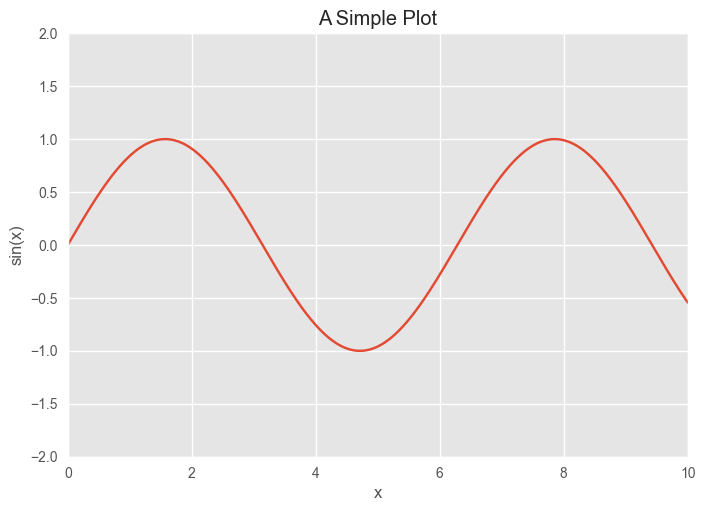
\includegraphics{../Figures/fig26-14.png}
    \caption{Example of using \texttt{ax.set} to set multiple properties at once}
    \label{fig26-14}
\end{figure}

\begin{pyc}
    ax = plt.axes()
    ax.plot(x, np.sin(x))
    ax.set(xlim=(0, 10), ylim=(-2, 2), xlabel='x', ylabel='sin(x)', title='A Simple Plot')
\end{pyc}
% \chapter{Simple Scatter Plots\label{Ch27}}
Another commonly used plot type is the simple scatter plot, a close cousin of the line
plot. Instead of points being joined by line segments, here the points are represented
individually with a dot, circle, or other shape.

\section{Scatter Plots with plt.plot}

In the previous chapter we looked at using plt.plot/ax.plot to produce line plots. It
turns out that this same function can produce scatter plots as well. The third argument in the function call is a character that represents the type of symbol used for the plotting. Just as you can specify options such as '-' or '--' to control the line style, the marker style has its own set of short string codes.

Most of the possibilities are fairly intuitive, and a number of
the more common ones are demonstrated here (see \autoref{Demonstration of point numbers}).

\figures{Demonstration of point numbers}

For even more possibilities, these character codes can be used together with line and
color codes to plot points along with a line connecting them.

\section{Scatter Plots with plt.scatter}
A second, more powerful method of creating scatter plots is the \verb|plt.scatter|\marginpar[plt.scatter]{plt.scatter} function, which can be used very similarly to the plt.plot function.

\begin{tcolorbox}
    The primary difference of plt.scatter from plt.plot is that it can be used to create
    scatter plots where the properties of each individual point (size, face color, edge color,
    etc.) can be individually controlled or mapped to data.
\end{tcolorbox}

\section{plot Versus scatter: A Note on Efficiency}
\begin{tcolorbox}
    Aside from the different features available in plt.plot and plt.scatter, why might
    you choose to use one over the other? While it doesn’t matter as much for small
    amounts of data, as datasets get larger than a few thousand points, plt.plot can be
    noticeably more efficient than plt.scatter. The reason is that plt.scatter has the
    capability to render a different size and/or color for each point, so the renderer must
    do the extra work of constructing each point individually. With plt.plot, on the
    other hand, the markers for each point are guaranteed to be identical, so the work of
    determining the appearance of the points is done only once for the entire set of data.
    For large datasets, this difference can lead to vastly different performance, and for
    this reason, plt.plot should be preferred over plt.scatter for large datasets.
\end{tcolorbox}

\section{Visualizing Uncertainties}
For any scientific measurement, accurate accounting of uncertainties is nearly as
important, if not more so, as accurate reporting of the number itself.(对任何一种科学测量方法来说,准确地衡量数据误差都是无比重要的事情,甚至比数据
本身还要重要。)
\subsection*{Basic Errorbars}
One standard way to visualize uncertainties is using an errorbar. A basic errorbar can
be created with a single Matplotlib function call, as shown in \autoref{An errorbar example}.

\figures{An errorbar example}

Using these additional options you can easily customize the aesthetics of your errorbar plot. I often find it helpful, especially in crowded plots, to make
the errorbars lighter than the points themselves.

\subsection*{Continuous Errors}
In some situations it is desirable to show errorbars on continuous quantities. Though
Matplotlib does not have a built-in convenience routine for this type of application,
it’s relatively easy to combine primitives like \verb|plt.plot| and \verb|plt.fill_between| for a
useful result.

Here we’ll perform a simple \emph{Gaussian process regression} which is a method of fitting a very flexible nonparametric function to data with a continuous measure of the uncertainty.


\autoref{Representing continuous uncertainty with filled regions}, the resulting figure gives an intuitive view into what the Gaussian process regression
algorithm is doing: in regions near a measured data point, the model is strongly constrained, and this is reflected in the small model uncertainties. In regions far from a
measured data point, the model is not strongly constrained, and the model uncertainties increase.

\figures{Representing continuous uncertainty with filled regions}
% \chapter{Density and Contour Plots\label{Ch28}}
Sometimes it is useful to display three-dimensional data in two dimensions using
contours or color-coded regions. There are three Matplotlib functions that can be
helpful for this task: plt.contour\marginpar[plt.contour]{plt.contour} for contour plots, plt.contourf\marginpar[plt.contourf]{plt.contourf} for filled contour
plots, and plt.imshow\marginpar[plt.imshow]{plt.imshow} for showing images.

\section{Visualizing a Three-Dimensional Function}
A contour plot can be created with the plt.contour function. It takes three arguments: a grid of x values, a grid of y values, and a grid of z values. The x and y values
represent positions on the plot, and the z values will be represented by the contour
levels. Perhaps the most straightforward way to prepare such data is to use the
np.meshgrid\marginpar[np.meshgrid]{np.meshgrid} function, which builds two-dimensional grids from one-dimensional
arrays.

Notice that when a single color is used, negative values are represented by dashed
lines and positive values by solid lines. Alternatively, the lines can be color-coded by
specifying a colormap with the cmap\marginpar[cmap]{cmap} argument.

Here we chose the RdGy (short for Red–Gray) colormap, which is a good choice for
divergent data: (i.e., data with positive and negative variation around zero).

Our plot is looking nicer, but the spaces between the lines may be a bit distracting.
We can change this by switching to a filled contour plot using the plt.contourf
function, which uses largely the same syntax as plt.contour.

Additionally, we'll add a plt.colorbar command, which creates an additional axis
with labeled color information for the plot (see \autoref{Visualizing three-dimensional data with filled contours}).

\figures{Visualizing three-dimensional data with filled contours}

One potential issue with this plot is that it is a bit splotchy: the color steps are discrete
rather than continuous, which is not always what is desired. This could be remedied
by setting the number of contours to a very high number, but this results in a rather
inefficient plot: Matplotlib must render a new polygon for each step in the level. A
better way to generate a smooth representation is to use the plt.imshow function,
which offers the interpolation argument to generate a smooth two-dimensional
representation of the data.

There are a few potential gotchas with plt.imshow, however(\important{以下这几条都很重要}):
\begin{itemize}
    \item It doesn't accept an x and y grid, so you must manually specify the extent [xmin,
                  xmax, ymin, ymax] of the image on the plot.
    \item By default it follows the standard image array definition where the origin is in the
          upper left, not in the lower left as in most contour plots. This must be changed
          when showing gridded data.
    \item It will automatically adjust the axis aspect ratio to match the input data; this can
          be changed with the aspect argument.
\end{itemize}

Finally, it can sometimes be useful to combine contour plots and image plots. For
example, here we'll use a partially transparent background image (with transparency
set via the alpha parameter) and overplot contours with labels on the contours themselves, using the plt.clabel function(see \autoref{Labeled contours on top of an image}):


\figures{Labeled contours on top of an image}

\begin{pyc}
    contours = plt.contour(X, Y, Z, 3, colors='black')
    plt.clabel(contours, inline=True, fontsize=8)
    plt.imshow(Z, extent=[0, 5, 0, 5], origin='lower', aspect='equal',
    cmap='RdGy', alpha=.5, interpolation='gaussian')
    plt.colorbar()
\end{pyc}

The combination of these three functions—plt.contour, plt.contourf, and
plt.imshow—gives nearly limitless possibilities for displaying this sort of three-
dimensional data within a two-dimensional plot.

\section{Histograms, Binnings, and Density}
A simple histogram can be a great first step in understanding a dataset.

The plt.hist docstring has more information on other available customization
options. I find this combination of \verb|histtype='stepfilled'| along with some transparency alpha to be helpful when comparing histograms of several distributions(see \autoref{Overplotting multiple histograms}).

\figures{Overplotting multiple histograms}

If you are interested in computing, but not displaying, the histogram (that is, counting the number of points in a given bin), you can use the \verb|np.histogram|\marginpar[np.histogram]{np.histogram} function.

\section{Two-Dimensional Histograms and Binnings}
Just as we create histograms in one dimension by dividing the number line into bins,
we can also create histograms in two dimensions by dividing points among two-dimensional bins.

\subsection*{plt.hist2d: Two-Dimensional Histogram}
One straightforward way to plot a two-dimensional histogram is to use Matplotlib's
\verb|plt.hist2d|\marginpar[plt.hist2d]{plt.hist2d} function.

Just as plt.hist has a counterpart in np.histogram, plt.hist2d has a counterpart in
np.histogram2d\marginpar[np.histogram2d]{np.histogram2d}.

\subsection*{plt.hexbin: Hexagonal Binnings}
The two-dimensional histogram creates a tesselation of squares across the axes.
Another natural shape for such a tesselation is the regular hexagon. For this purpose,
Matplotlib provides the plt.hexbin routine, which represents a two-dimensional
dataset binned within a grid of hexagons.

plt.hexbin has a number of additional options, including the ability to specify
weights for each point and to change the output in each bin to any NumPy aggregate
(mean of weights, standard deviation of weights, etc.).

\subsection*{Kernel Density Estimation}
Another common method for estimating and representing densities in multiple
dimensions is \textbf{kernel density estimation}\marginpar[kernel density estimation]{kernel density estimation} (KDE). Now I'll simply mention that KDE can be thought of as a way to
“smear out” the points in space and add up the result to obtain a smooth function.

KDE has a smoothing length that effectively slides the knob between detail and
smoothness (one example of the ubiquitous bias–variance trade-off).
% \chapter{Customizing Plot Legends\label{Ch29}}
Plot legends give meaning to a visualization, assigning meaning to the various plot
elements.

We can specify the location and turn on the frame. We can use the ncol command to specify the number of columns in the legend. And we can use a rounded box (fancybox) or add a shadow, change the transparency
(alpha value) of the frame, or change the padding around the text(see \autoref{A fancybox plot legend}).

\figures{A fancybox plot legend}
\section{Choosing Elements for the Legend}
As we have already seen, by default the legend includes all labeled elements from the
plot. If this is not what is desired, we can fine-tune which elements and labels appear
in the legend by using the objects returned by plot commands. plt.plot is able to
create multiple lines at once, and returns a list of created line instances. Passing any of
these to plt.legend will tell it which to identify, along with the labels we'd like to
specify.

Notice that the legend ignores all elements without a label attribute set.


\section{Legend for Size of Points}
Sometimes the legend defaults are not sufficient for the given visualization. For example, perhaps you're using the size of points to mark certain features of the data, and
want to create a legend reflecting this. (可视化气泡图,需要将图里的大小也同步调整)

The legend will always reference some object that is on the plot, so if we'd like to display a particular shape we need to plot it. In this case, the objects we want (gray circles) are not on the plot, so we fake them by plotting empty lists. Recall that the
legend only lists plot elements that have a label specified.

\section{Multiple Legends}

Sometimes when designing a plot you'd like to add multiple legends to the same axes.
Unfortunately, Matplotlib does not make this easy: via the standard legend interface,
it is only possible to create a single legend for the entire plot. If you try to create a
second legend using plt.legend or ax.legend, it will simply override the first one.
We can work around this by creating a new legend artist from scratch (\verb|Artist|\marginpar[Artist]{Artist} is the
base class Matplotlib uses for visual attributes), and then using the lower-level
\verb|ax.add_artist| method to manually add the second artist to the plot.

\figures{A split plot legend}

\begin{pyc}
    fig, ax = plt.subplots()
    lines = []
    styles = ['-', '--', '-.', ':']
    x = np.linspace(0, 10, 1000)
    for i in range(4):
    lines += ax.plot(x, np.sin(x - i * np.pi / 2),
    styles[i], color='black')
    ax.legend(lines[:2], ['line A', 'line B'], loc='upper right')

    ax.axis('equal')

    from matplotlib.legend import Legend
    leg = Legend(ax, lines[2:], ['line C', 'line D'], loc='lower right')
    ax.add_artist(leg)
\end{pyc}
% \chapter{Customizing Colorbars\label{Ch30}}
Plot legends identify discrete labels of discrete points. For continuous labels based on
the color of points, lines, or regions, a labeled colorbar can be a great tool. In Matplotlib, a colorbar is drawn as a separate axes that can provide a key for the meaning
of colors in a plot.

As we have seen several times already, the simplest colorbar can be created with the
plt.colorbar\marginpar[plt.colorbar]{plt.colorbar} function.

\section{Customizing Colorbars}
The colormap can be specified using the cmap argument to the plotting function that
is creating the visualization. The names of available colormaps are in the \verb|plt.cm| namespace.

\subsection*{Choosing the Colormap}
Broadly, you should be aware of three different categories of colormaps:
\begin{itemize}
    \item  \textbf{Sequential colormaps}(顺序配色方案): These are made up of one continuous sequence of colors (e.g., binary or
          viridis).
    \item  \textbf{Divergent colormaps}(互逆配色方法): These usually contain two distinct colors, which show positive and negative deviations from a mean (e.g., RdBu or PuOr).
    \item  \textbf{Qualitative colormaps}(定性配色方法): These mix colors with no particular sequence (e.g., rainbow or jet).
\end{itemize}

The jet colormap, which was the default in Matplotlib prior to version 2.0, is an
example of a qualitative colormap. Its status as the default was quite unfortunate,
because qualitative maps are often a poor choice for representing quantitative data.
\tips{Among the problems is the fact that qualitative maps usually do not display any uniform progression in brightness as the scale increases.}
We can see this by converting the jet colorbar into black and white (see \autoref{The jet colormap and its uneven luminance scale})

\figures{The jet colormap and its uneven luminance scale}

Notice the bright stripes in the grayscale image. Even in full color, this uneven brightness means that the eye will be drawn to certain portions of the color range, which
will potentially emphasize unimportant parts of the dataset. It’s better to use a colormap such as viridis (the default as of Matplotlib 2.0), which is specifically constructed to have an even brightness variation across the range; thus, it not only plays well
with our color perception, but also will translate well to grayscale printing.

For other situations, such as showing positive and negative deviations from some
mean, dual-color colorbars such as RdBu (Red–Blue) are helpful. However, as you can
see in \autoref{The RdBu colormap and its luminance}, it’s important to note that the positive/negative information will be
lost upon translation to grayscale!

\figures{The RdBu colormap and its luminance}
更多关于绘图的可以参考,\href{https://journals.plos.org/ploscompbiol/article?id=10.1371/journal.pcbi.1003833}{Ten Simple Rules for Better Figures}.
\subsection*{Color Limits and Extensions}
Matplotlib allows for a large range of colorbar customization. The colorbar itself is
simply an instance of plt.Axes, so all of the axes and tick formatting tricks we’ve seen
so far are applicable. The colorbar has some interesting flexibility: for example, we
can narrow the color limits and indicate the out-of-bounds values with a triangular
arrow at the top and bottom by setting the extend property.

\subsection*{Discrete Colorbars}

Colormaps are by default continuous, but sometimes you’d like to represent discrete
values. The easiest way to do this is to use the \verb|plt.cm.get_cmap|\footnote{MatplotlibDeprecationWarning: The get\_cmap function was deprecated in Matplotlib 3.7 and will be removed two minor releases later. Use ``matplotlib.colormaps[name]`` or ``matplotlib.colormaps.get\_cmap(obj)`` instead.} function and pass the
name of a suitable colormap along with the number of desired bins.

\section{Example: Handwritten Digits}
Because each digit is defined by the hue of its 64 pixels, we can consider each digit to
be a point lying in 64-dimensional space: each dimension represents the brightness of
one pixel. Visualizing such high-dimensional data can be difficult, but one way to
approach this task is to use a dimensionality reduction technique such as manifold
learning to reduce the dimensionality of the data while maintaining the relationships
of interest. Dimensionality reduction is an example of unsupervised machine learning, and we will discuss it in more detail in \autoref{Ch37}.
% \chapter{Multiple Subplots\label{Ch31}}
Sometimes it is helpful to compare different views of data side by side. To this end,
Matplotlib has the concept of subplots: groups of smaller axes that can exist together
within a single figure. These subplots might be insets(画中画), grids of plots, or other more
complicated layouts. In this chapter we'll explore four routines for creating subplots
in Matplotlib.
\section{plt.axes: Subplots by Hand}
The most basic method of creating an axes is to use the plt.axes\marginpar[plt.axes]{plt.axes} function. As we've
seen previously, by default this creates a standard axes object that fills the entire figure. plt.axes also takes an optional argument that is a list of four numbers in the
figure coordinate system (\verb|[left, bottom, width, height]|), which ranges from 0 at
the bottom left of the figure to 1 at the top right of the figure.

For example, we might create an inset axes at the top-right corner of another axes by
setting the x and y position to 0.65 (that is, starting at 65\% of the width and 65% of
the height of the figure) and the x and y extents to 0.2 (that is, the size of the axes is
20\% of the width and 20\% of the height of the figure)(see \autoref{Example of an inset axes}).

The equivalent of this command within the object-oriented interface is \verb|fig.add_axes|\marginpar[fig.add\_axes]{fig.add\_axes}.
\begin{figure}
    \centering
    \begin{subfigure}[b]{.45\textwidth}
        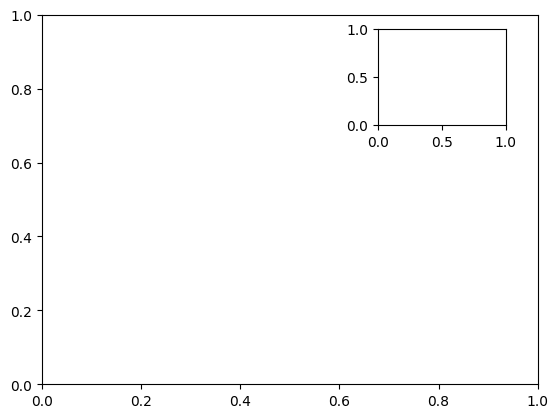
\includegraphics[width=\textwidth]{../Figures/Example of an inset axes.png}
        \caption{Example of an inset axes}
        \label{Example of an inset axes}
    \end{subfigure}
    \hfill
    \begin{subfigure}[b]{.45\textwidth}
        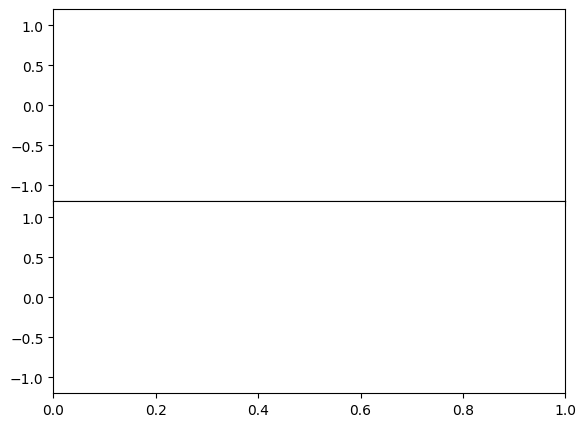
\includegraphics[width=\textwidth]{../Figures/Vertically stacked axes example.png}
        \caption{Vertically stacked axes example}
        \label{Vertically stacked axes example}
    \end{subfigure}
    \caption{Subplots by Hand}
\end{figure}
\section{plt.subplot: Simple Grids of Subplots}
Aligned columns or rows of subplots are a common enough need that Matplotlib has
several convenience routines that make them easy to create. The lowest level of these
is \verb|plt.subplot|\marginpar[plt.subplot]{plt.subplot}, which creates a single subplot within a grid. As you can see, this
command takes three integer arguments—the number of rows, the number of columns, and the index of the plot to be created in this scheme, which runs from the
upper left to the bottom right.(see \autoref{A plt.subplot example})

\begin{figure}
    \centering
    \begin{subfigure}[b]{.45\textwidth}
        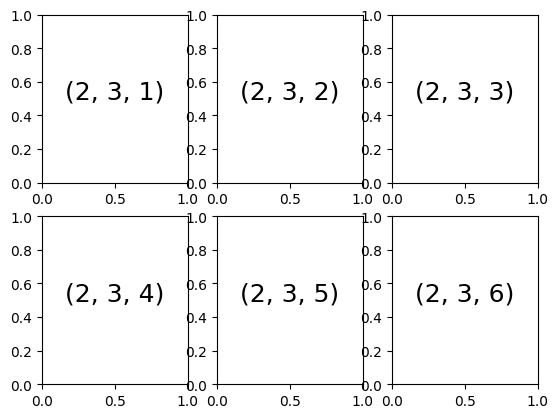
\includegraphics[width=\textwidth]{../Figures/A plt.subplot example.png}
        \caption{A plt.subplot example}
        \label{A plt.subplot example}
    \end{subfigure}
    \hfill
    \begin{subfigure}[b]{.45\textwidth}
        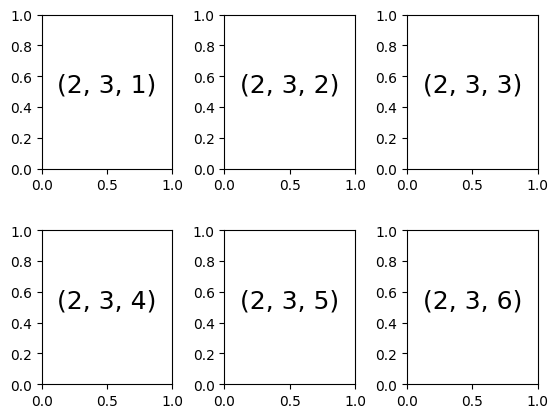
\includegraphics[width=\textwidth]{../Figures/plt.subplot with adjusted margins.png}
        \caption{plt.subplot with adjusted margins}
        \label{plt.subplot with adjusted margins}
    \end{subfigure}
    \caption{plt.subplot: Simple Grids of Subplots}
\end{figure}

The command \verb|plt.subplots_adjust| can be used to adjust the spacing between
these plots. The following code uses the equivalent object-oriented command,
\verb|fig.add_subplot|; \autoref{plt.subplot with adjusted margins} shows the result.

Here we've used the hspace and wspace arguments of \verb|plt.subplots_adjust|, which
specify the spacing along the height and width of the figure, in units of the subplot
size (in this case, the space is 40\% of the subplot width and height).
\section{plt.subplots: The Whole Grid in One Go}
The approach just described quickly becomes tedious when creating a large grid of
subplots, especially if you'd like to hide the x- and y-axis labels on the inner plots. For
this purpose, \verb|plt.subplots|\marginpar[plt.subplots]{plt.subplots} is the easier tool to use (note the s at the end of
subplots). Rather than creating a single subplot, this function creates a full grid of
subplots in a single line, returning them in a NumPy array. The arguments are the
number of rows and number of columns, along with optional keywords sharex and
sharey, which allow you to specify the relationships between different axes.

In comparison to plt.subplot, plt.subplots is more consistent with Python's conventional zero-based indexing, whereas plt.subplot uses MATLAB-style one-based
indexing.
\section{plt.GridSpec: More Complicated Arrangements}
To go beyond a regular grid to subplots that span multiple rows and columns,
\verb|plt.GridSpec|\marginpar[plt.GridSpec]{plt.GridSpec} is the best tool. plt.GridSpec does not create a plot by itself; it is
rather a convenient interface that is recognized by the plt.subplot command.

\begin{pyc}
    grid = plt.GridSpec(2, 3, wspace=.4, hspace=.3)
    plt.subplot(grid[0, 0])
    plt.subplot(grid[0, 1:])
    plt.subplot(grid[1, :2])
    plt.subplot(grid[1, 2])
    plt.show()
\end{pyc}

This type of flexible grid alignment has a wide range of uses. I most often use it when
creating multiaxes histogram plots.
\figures{Visualizing multidimensional distributions with plt.GridSpec}
% \chapter{Text and Annotation\label{Ch32}}
Creating a good visualization involves guiding the reader so that the figure tells a
story. In some cases, this story can be told in an entirely visual manner, without the
need for added text, but in others, small textual cues and labels are necessary. Perhaps
the most basic types of annotations you will use are axes labels and titles, but the
options go beyond this.

When we're visualizing data, it is often useful to annotate certain features of
the plot to draw the reader's attention. This can be done manually with the \verb|plt.text|\marginpar[plt.text]{plt.text}/
\verb|ax.text|\marginpar[ax.text]{ax.text} functions, which will place text at a particular $x$/$y$ value.

The ax.text method takes an $x$ position, a $y$ position, a string, and then optional keywords specifying the color, size, style, alignment, and other properties of the text.
Here we used \verb|ha='right'| and \verb|ha='center'|, where \verb|ha| is short for \emph{horizontal alignment}.

\section{Transforms and Text Position}
In the previous example, we anchored our text annotations to data locations. Sometimes it's preferable to anchor the text to a fixed position on the axes or figure, independent of the data. In Matplotlib, this is done by modifying the transform.

Matplotlib makes use of a few different coordinate systems: a data point at
$(x, y) = (1, 1)$ corresponds to a certain location on the axes or figure, which in turn
corresponds to a particular pixel on the screen. Mathematically, transforming
between such coordinate systems is relatively straightforward, and Matplotlib has a
well-developed set of tools that it uses internally to perform these transforms.

A typical user rarely needs to worry about the details of the transforms, but it is helpful knowledge to have when considering the placement of text on a figure. There are
three predefined transforms that can be useful in this situation:
\begin{itemize}
    \item \textbf{ax.transData}: Transform associated with data coordinates
    \item \textbf{ax.transAxes}: Transform associated with the axes (in units of axes dimensions)
    \item \textbf{fig.transFigure}: Transform associated with the figure (in units of figure dimensions)
\end{itemize}

\figures{Comparing Matplotlib coordinate systems}

The transData coordinates give the usual data coordinates associated with the x- and
y-axis labels. The transAxes coordinates give the location from the bottom-left corner of the axes (the white box), as a fraction of the total axes size. The transFig
ure coordinates are similar, but specify the position from the bottom-left corner of
the figure (the gray box) as a fraction of the total figure size.

\important{Notice now that if we change the axes limits, it is only the transData coordinates that
    will be affected, while the others remain stationary. }

\section{Arrows and Annotation}
Along with tickmarks and text, another useful annotation mark is the simple arrow.

I'd suggest using the \verb|plt.annotate|\marginpar[plt.annotate]{plt.annotate} function, which creates some text and an arrow and allows the arrows to be very flexibly
specified.

More discussion and examples of available arrow and annotation styles can be found
in the Matplotlib \href{https://matplotlib.org/stable/tutorials/text/annotations.html}{Annotations tutorial}.

\figures{Annotated average birth rates by day}
% \chapter{Customizing Ticks\label{}}
Matplotlib's default tick locators and formatters are designed to be generally sufficient
in many common situations, but are in no way optimal for every plot.

Before we go into examples, however, let's talk a bit more about the object hierarchy
of Matplotlib plots. Matplotlib aims to have a Python object representing everything
that appears on the plot: for example, recall that the Figure is the bounding box
within which plot elements appear. Each Matplotlib object can also act as a container
of subobjects: for example, each Figure can contain one or more Axes objects, each
of which in turn contains other objects representing plot contents.

The tickmarks are no exception. Each axes has attributes xaxis and yaxis, which in
turn have attributes that contain all the properties of the lines, ticks, and labels that
make up the axes.
\section{Major and Minor Ticks}
Within each axes, there is the concept of a major tickmark, and a minor tickmark. As
the names imply, major ticks are usually bigger or more pronounced, while minor
ticks are usually smaller. By default, Matplotlib rarely makes use of minor ticks, but
one place you can see them is within logarithmic plots.


These tick properties—locations and labels, that is—can be customized by setting the
\verb|formatter|\marginpar[formatter]{formatter} and \verb|locator|\marginpar[locator]{locator} objects of each axis.



\begin{pyc}
    ax.xaxis.get_major_locator()
    ax.xaxis.get_minor_locator()
    ax.xaxis.get_major_formatter()
    ax.xaxis.get_minor_formatter()
\end{pyc}

\section{Hiding Ticks or Labels}
Perhaps the most common tick/label formatting operation is the act of hiding ticks or
labels. This can be done using \verb|plt.NullLocator| and \verb|plt.NullFormatter|. Having no ticks at
all can be useful in many situations—for example, when you want to show a grid of
images.

\section{Reducing or Increasing the Number of Ticks}
One common problem with the default settings is that smaller subplots can end up
with crowded labels. Particularly for the x-axis ticks, the numbers nearly overlap, making them quite difficult to decipher. One way to adjust this is with \verb|plt.MaxNLocator|, which allows us to
specify the maximum number of ticks that will be displayed.

\section{Fancy Tick Formats}
Matplotlib's default tick formatting can leave a lot to be desired: it works well as a
broad default, but sometimes you'd like to do something different. 比如说需要绘制 $\pi$ 作为刻度,而不是整数或者说是小数表示的 $\pi$。

We can do this by setting a
\verb|MultipleLocator|\marginpar[MultipleLocator]{MultipleLocator}, which locates ticks at a multiple of the number we provide.

we can change the tick formatter. There's no built-in formatter for what we want to do, so
we'll instead use \verb|plt.FuncFormatter|, which accepts a user-defined function giving
fine-grained control over the tick outputs

\section{Summary of Formatters and Locators}
We've seen a couple of the available formatters and locators; I'll conclude this chapter
by listing all of the built-in locator options (\autoref{Matplotlib locator options}) and formatter options
(\autoref{Matplotlib formatter options}).

\begin{table}
    \centering
    \caption{Matplotlib locator options}
    \label{Matplotlib locator options}
    \begin{tabular}{ll}
        \hline
        Locator class    & Description                                             \\
        \hline
        NullLocator      & No ticks                                                \\
        FixedLocator     & Tick locations are fixed                                \\
        IndexLocator     & Locator for index plots (e.g., where x = range(len(y))) \\
        LinearLocator    & Evenly spaced ticks from min to max                     \\
        LogLocator       & Logarithmically spaced ticks from min to max            \\
        MultipleLocator  & Ticks and range are a multiple of base                  \\
        MaxNLocator      & Finds up to a max number of ticks at nice locations     \\
        AutoLocator      & (Default) MaxNLocator with simple defaults              \\
        AutoMinorLocator & Locator for minor ticks                                 \\
        \hline
    \end{tabular}
\end{table}

\begin{table}
    \centering
    \caption{Matplotlib formatter options}
    \label{Matplotlib formatter options}
    \begin{tabular}{ll}
        \hline
        Formatter class    & Description                             \\
        \hline
        NullFormatter      & No labels on the ticks                  \\
        IndexFormatter     & Set the strings from a list of labels   \\
        FixedFormatter     & Set the strings manually for the labels \\
        FuncFormatter      & User-defined function sets the labels   \\
        FormatStrFormatter & Use a format string for each value      \\
        ScalarFormatter    & Default formatter for scalar values     \\
        LogFormatter       & Default formatter for log axes          \\
        \hline
    \end{tabular}
\end{table}
% \chapter{Customizing Matplotlib: Configurations and Stylesheets\label{Ch34}}
While many of the topics covered in previous chapters involve adjusting the style of
plot elements one by one, Matplotlib also offers mechanisms to adjust the overall
style of a chart all at once. In this chapter we'll walk through some of Matplotlib's runtime configuration (\textbf{rc}) options, and take a look at the stylesheets feature, which
contains some nice sets of default configurations.

\section{Plot Customization by Hand}

\section{Changing the Defaults: rcParams}
Each time Matplotlib loads, it defines a runtime configuration containing the default
styles for every plot element you create. This configuration can be adjusted at any
time using the \verb|plt.rc|\marginpar[plt.rc]{plt.rc} convenience routine.

Optionally, these settings can be saved in a \textbf{.matplotlibrc} file.

\section{Stylesheets}
A newer mechanism for adjusting overall chart styles is via Matplotlib's style module, which includes a number of default stylesheets, as well as the ability to create and
package your own styles. These stylesheets are formatted similarly to the \textbf{.matplotlibrc}
files mentioned earlier, but must be named with a \textbf{.mplstyle} extension.
Even if you don't go as far as creating your own style, you may find what you're looking for in the built-in stylesheets. \verb|plt.style.available| contains a list of the available styles.

The standard way to switch to a stylesheet is to call \verb|style.use|.

\important{But keep in mind that this will change the style for the rest of the Python session!
    Alternatively, you can use the style context manager, which sets a style temporarily.}

\subsection*{Default Style}
Matplotlib's default style was updated in the version 2.0 release.

\subsection*{FiveThirtyEight Style}
The fivethirtyeight style mimics the graphics found on the popular \href{https://fivethirtyeight.com/}{FiveThirtyEight website}. It is typified by bold colors, thick lines, and transparent axes.

\subsection*{ggplot Style}
The ggplot package in the R language is a popular visualization tool among data scientists. Matplotlib's ggplot style mimics the default styles from that package.

\subsection*{Bayesian Methods for Hackers Style}
There is a neat short online book called \href{https://dataorigami.net/Probabilistic-Programming-and-Bayesian-Methods-for-Hackers/}{Probabilistic Programming and Bayesian Methods for Hackers} by Cameron Davidson-Pilon that features figures created with
Matplotlib, and uses a nice set of rc parameters to create a consistent and visually
appealing style throughout the book. This style is reproduced in the bmh stylesheet.

\subsection*{Dark Background Style}
For figures used within presentations, it is often useful to have a dark rather than light
background. The \verb|dark_background| style provides this.

\subsection*{Grayscale Style}
You might find yourself preparing figures for a print publication that does not accept
color figures. For this, the grayscale style can be useful.

\subsection*{Seaborn Style}
Matplotlib also has several stylesheets inspired by the Seaborn library. I've found these settings to be very nice, and tend to use
them as defaults in my own data exploration
% \chapter{Three-Dimensional Plotting in Matplotlib\label{Ch35}}
Three-
dimensional plots are enabled by importing the mplot3d toolkit, included with the
main Matplotlib installation.

Once this submodule is imported, a three-dimensional axes can be created by passing
the keyword \verb|projection='3d'| to any of the normal axes creation routines.

Three-dimensional plotting is one of the functionalities that
benefits immensely from viewing figures interactively rather than statically, in the
notebook; recall that to use interactive figures, you can use \verb|%matplotlib notebook|
rather than \verb|%matplotlib inline| when running this code.

\section{Three-Dimensional Points and Lines}
The most basic three-dimensional plot is a line or collection of scatter plots created
from sets of $(x, y, z)$ triples. In analogy with the more common two-dimensional plots
discussed earlier, these can be created using the \verb|ax.plot3D| and \verb|ax.scatter3D| functions. The call signature for these is nearly identical to that of their two-dimensional
counterparts.

\section{Three-Dimensional Contour Plots}
mplot3d contains tools to
create three-dimensional relief(晕渲) plots using the same inputs. Like \verb|ax.contour|, \verb|ax.contour3D| requires all the input data to be in the form of two-dimensional regular grids,
with the z data evaluated at each point.

Sometimes the default viewing angle is not optimal, in which case we can use the
\verb|view_init| method to set the elevation(角度) and azimuthal angles(方向角).

\section{Wireframes(线框图) and Surface Plots}
Two other types of three-dimensional plots that work on gridded data are wireframes
and surface plots. These take a grid of values and project it onto the specified three-
dimensional surface, and can make the resulting three-dimensional forms quite easy
to visualize.

A surface plot is like a wireframe plot, but each face of the wireframe is a filled polygon. Adding a colormap to the filled polygons can aid perception of the topology of
the surface being visualized.

Though the grid of values for a surface plot needs to be two-dimensional, it need not
be rectilinear(直角坐标系).

\section{Surface Triangulations}
For some applications, the evenly sampled grids required by the preceding routines
are too restrictive. In these situations, triangulation-based plots can come in handy.
What if rather than an even draw from a Cartesian or a polar grid, we instead have a
set of random draws?


The function that will help us in this case is
\verb|ax.plot_trisurf|, which creates a surface by first finding a set of triangles formed
between adjacent points.



% \chapter{Visualization with Seaborn\label{Ch36}}
\section{Exploring Seaborn Plots}
The main idea of Seaborn is that it provides high-level commands to create a variety
of plot types useful for statistical data exploration, and even some statistical model
fitting.

Let’s take a look at a few of the datasets and plot types available in Seaborn. Note that
all of the following could be done using raw Matplotlib commands (this is, in fact,
what Seaborn does under the hood), but the Seaborn API is much more convenient.

\subsection*{Histograms, KDE, and Densities}
Often in statistical data visualization, all you want is to plot histograms and joint distributions of variables. We have seen that this is relatively straightforward in Matplotlib.


Rather than just providing a histogram as a visual output, we can get a smooth estimate of the distribution using kernel density estimation,
which Seaborn does with \verb|sns.kdeplot|.

If we pass $x$ and $y$ columns to kdeplot, we instead get a two-dimensional visualization of the joint density.

We can see the joint distribution and the marginal distributions together using
\verb|sns.jointplot|.

\subsubsection*{Pair Plots}
When you generalize joint plots to datasets of larger dimensions, you end up with
\textbf{pair plots}(矩阵图). These are very useful for exploring correlations between multidimensional
data, when you’d like to plot all pairs of values against each other.

Visualizing the multidimensional relationships among the samples is as easy as calling \verb|sns.pairplot|.

\subsection*{Faceted Histograms}
Sometimes the best way to view data is via histograms of subsets. Seaborn’s \verb|FacetGrid| makes this simple.

\section{Categorical Plots}
Categorical plots can be useful for this kind of visualization as well. These allow you
to view the distribution of a parameter within bins defined by any other parameter.

\subsection*{Joint Distributions}
Similar to the pair plot we saw earlier, we can use sns.jointplot to show the joint
distribution between different datasets, along with the associated marginal distributions.(see \autoref{A joint distribution plot})

The joint plot can even do some automatic kernel density estimation and regression, as shown in \autoref{A joint distribution plot with a regression fit}.

\begin{figure}
    \centering
    \begin{subfigure}[b]{.45\textwidth}
        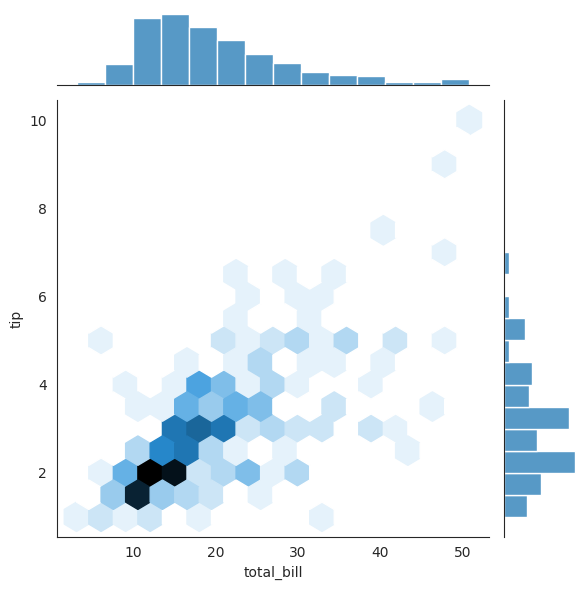
\includegraphics[width=\textwidth]{../Figures/A joint distribution plot.png}
        \caption{A joint distribution plot}
        \label{A joint distribution plot}
    \end{subfigure}
    \hfill
    \begin{subfigure}[b]{.45\textwidth}
        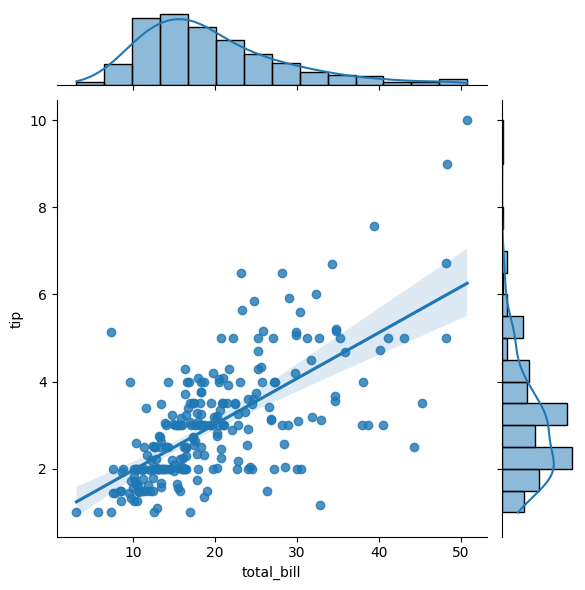
\includegraphics[width=\textwidth]{../Figures/A joint distribution plot with a regression fit.png}
        \caption{A joint distribution plot with a regression fit}
        \label{A joint distribution plot with a regression fit}
    \end{subfigure}
    \caption{Joint Distributions}
\end{figure}

\subsection*{Bar Plots}
Time series can be plotted using \verb|sns.catplot|. We can learn more by looking at the factor of data of each of these categories.

For more information on plotting with Seaborn, see the \href{http://seaborn.pydata.org/}{Seaborn documentation}, and
particularly the \href{https://seaborn.pydata.org/examples/index.html}{example gallery}.

\section{用Basemap可视化地理数据}
地理数据可视化是数据科学中一种十分常见的可视化类型。Matplotlib 做此类可视化的主
要工具是 Basemap 工具箱。

\subsection{地图投影}
当你想使用地图时,首先要做的就是确定地图的投影类型。你可能已经知道,像地球这样
的球体,可以通过球面透视法将三维球面投影成一个二维平面,不会造成变形,也不会破坏其连续性。

\subsubsection*{圆柱投影}
圆柱投影(cylindrical projection)是最简单的地图投影类型,纬度线与经度线分别映射
成水平线与竖直线。采用这种投影类型的话,赤道区域的显示效果非常好,但是南北极
附近的区域就会严重变形。由于纬度线的间距会因圆柱投影的不同而不同,所以就有了
不同的投影属性和南北极附近不同的变形程度。等距圆柱投
影(cyl),不同纬度在子午线方向的间距保持不变。另外两种圆柱投影是墨卡托(Mercator,
projection='merc')投影和圆柱等积(cylindrical equal-area,projection='cea')投影。
\subsubsection*{伪圆柱投影}
伪圆柱投影(pseudo-cylindrical projection)的经线不再必须是竖直的,这样可以使南北
极附近的区域更加真实。摩尔威德(Mollweide,projection='moll')投影就是这类投影
的典型代表,它所有的经线都是椭圆弧线,如图 4-105 所示。这么做是为了保留地图原
貌——虽然南北极附近的区域还有一些变形,但是通过一些区域小图可以反映真实情况。
其他伪圆柱投影类型有正弦(sinusoidal,projection='sinu')投影和罗宾森(Robinson,
projection='robin')投影。
\subsubsection*{透视投影}
透视投影(perspective projection)是从某一个透视点对地球进行透视获得的投影,就好像
你站在太空中某一点给地球照相一样(通过技术处理,有些投影类型的透视点可以放在地
球上)。一个典型示例是正射(orthographic,projection='ortho')投影,从无限远处观
察地球的一侧。因此,这种投影一次只能显示半个地球。其他的透视投影类型还有球心(gnomonic,projection='gnom') 投 影 和 球 极 平 面(stereographic,projection='stere')
投影。这些投影经常用于显示地图的较小面积区域。

\subsubsection*{圆锥投影}
圆锥投影(conic projection)是先将地图投影成一个圆锥体,然后再将其展开。这样做虽
然可以获得非常好的局部效果,但是远离圆锥顶点的区域可能会严重变形。一个典型示例
就是兰勃特等角圆锥投影(Lambert conformal conic projection,projection='lcc'),也就
是我们之前见到的北美洲地图。这种方法将地图投影成一个由两条标准纬线(用 Basemap
里的 lat\_1 与 lat\_2 参数设置)构成的圆锥,这两条纬线距离是经过精心挑选的,在两条
标准纬线之内比例尺逐渐减小,在两线之外的比例尺逐渐增大。其他常用的圆锥投影还有
等距圆锥(equidistant conic,projection='eqdc')投影和阿尔伯斯等积圆锥(Albers equalarea,projection='aea')投影。圆锥投影和透视投影一样,适合显示较
小与中等区域的地图。
% \part{Machine Learning}
% \chapter{What Is Machine Learning?\label{Ch37}}
\section{Qualitative Examples of Machine Learning Applications}
\subsection*{Dimensionality Reduction: Inferring Structure of Unlabeled Data}
\subsection*{}
\section{Summary}
In short, we saw the following:
\begin{itemize}
    \item Supervised learning: Models that can predict labels based on labeled training data
          \begin{itemize}
              \item Classification: Models that predict labels as two or more discrete categories
              \item Regression: Models that predict continuous labels
          \end{itemize}
    \item Unsupervised learning: Models that identify structure in unlabeled data
          \begin{itemize}
              \item Clustering: Models that detect and identify distinct groups in the data
              \item Dimensionality reduction: Models that detect and identify lower-dimensional structure in higher-dimensional data
          \end{itemize}
\end{itemize}
% \chapter{Introducing Scikit-Learn\label{Ch38}}
\section{Data Representation in Scikit-Learn}
Consider the Iris dataset, each row of the data refers to a single observed flower, and the number of rows
is the total number of flowers in the dataset. In general, we will refer to the rows of
the matrix as \textbf{samples}, and the number of rows as \verb|n_samples|.

Likewise, each column of the data refers to a particular quantitative piece of information that describes each sample. In general, we will refer to the columns of the matrix
as \textbf{features}, and the number of columns as \verb|n_features|.

\subsection*{The Features Matrix}
The table layout makes clear that the information can be thought of as a two-
dimensional numerical array or matrix, which we will call the \textbf{features matrix}. By convention, this matrix is often stored in a variable named X. The features matrix is
assumed to be two-dimensional, with shape \verb|[n_samples, n_features]|, and is most
often contained in a NumPy array or a Pandas DataFrame, though some Scikit-Learn
models also accept SciPy sparse matrices.

\subsection*{The Target Array}
In addition to the feature matrix X, we also generally work with a label or target array,
which by convention we will usually call y. The target array is usually one-
dimensional, with length \verb|n_samples|, and is generally contained in a NumPy array or
Pandas Series. The target array may have continuous numerical values, or discrete
classes/labels. While some Scikit-Learn estimators do handle multiple target values in
the form of a two-dimensional, \verb|[n_samples, n_targets]| target array, we will primarily be working with the common case of a one-dimensional target array.

\section{The Estimator API}
\subsection*{Basics of the API}
Most commonly, the steps in using the Scikit-Learn Estimator API are as follows:
\begin{enumerate}
    \item Choose a class of model by importing the appropriate estimator class from Scikit-
          Learn.
    \item Choose model hyperparameters by instantiating this class with desired values.
    \item Arrange data into a features matrix and target vector.
    \item Fit the model to your data by calling the fit method of the model instance.
    \item Apply the model to new data:
          \begin{itemize}
              \item For supervised learning, often we predict labels for unknown data using the
                    \verb|predict| method.
              \item For unsupervised learning, we often transform or infer properties of the data
                    using the \verb|transform| or \verb|predict| method.
          \end{itemize}
\end{enumerate}

\subsection*{Supervised Learning Example: Simple Linear Regression}
\subsubsection*{Choose model hyperparameters}
\important{An important point is that a class of model is not the same as an instance of a model.}

Once we have decided on our model class, there are still some options open to us.
Depending on the model class we are working with, we might need to answer one or
more questions like the following:

\begin{itemize}
    \item Would we like to fit for the offset (i.e., y-intercept)?
    \item Would we like the model to be normalized?
    \item Would we like to preprocess our features to add model flexibility?
    \item What degree of regularization would we like to use in our model?
    \item How many model components would we like to use?
\end{itemize}

These are examples of the important choices that must be made once the model class is
selected. These choices are often represented as hyperparameters, or parameters that
must be set before the model is fit to data.

\subsubsection*{Supervised Learning Example: Iris Classification}
We will use a simple generative model known as \textbf{Gaussian naive Bayes}\marginpar[Gaussian naive Bayes]{Gaussian naive Bayes},
which proceeds by assuming each class is drawn from an axis-aligned Gaussian distribution. Because it is so fast and has no hyperparameters to choose,
\tips{Gaussian naive Bayes is often a good model to use as a baseline
    classification, before exploring whether improvements can be found through more
    sophisticated models.}
% \chapter{Hyperparameters and Model Validation\label{Ch39}}
\section{Thinking About Model Validation}
In principle, model validation is very simple: after choosing a model and its hyperparameters, we can estimate how effective it is by applying it to some of the training
data and comparing the predictions to the known values.
\subsection*{Model Validation the Right Way: Holdout Sets}
A better sense of a model's performance can be found by using
what's known as a \textit{holdout set}: that is, we hold back some subset of the data from the
training of the model, and then use this holdout set to check the model's performance.
\subsection*{Model Validation via Cross-Validation}
One disadvantage of using a holdout set for model validation is that we have lost a
portion of our data to the model training.

One way to address this is to use cross-validation; that is, to do a sequence of fits
where each subset of the data is used both as a training set and as a validation set.

cikit-Learn implements a number of cross-validation schemes that are useful in particular situations; these are implemented via iterators in the \verb|model_selection| module. For example, we might wish to go to the extreme case in which our number of
folds is equal to the number of data points: that is, we train on all points but one in
each trial. This type of cross-validation is known as \textit{leave-one-out}\marginpar[留一验证]{留一验证} cross validation.

\section{Selecting the Best Model}
\subsection*{The Bias-Variance Trade-off}
Fundamentally, finding “the best model” is about finding a sweet spot in the trade-off
between bias and variance.

欠拟合的模型会有较高的偏差(bias),过拟合的模型甚至拟合了数据中的随机误差,这样的模型具有较高的方差(variance)。

The $R^2$ score, or coefficient of determination, measures how
well a model performs relative to a simple mean of the target values. $R^2 = 1$ indicates
a perfect match, $R^2 = 0$ indicates the model does no better than simply taking the
mean of the data, and \important{negative values mean even worse models}.

If we imagine that we have some ability to tune the model complexity, we would
expect the training score and validation score to behave as illustrated in \autoref{fig39-5},
often called a validation curve, and we see the following features:
\begin{itemize}
      \item The training score is everywhere higher than the validation score. This is generally the case: the model will be a better fit to data it has seen than to data it has
            not seen.
      \item For very low model complexity (a high-bias model), the training data is underfit,
            which means that the model is a poor predictor both for the training data and for
            any previously unseen data.
      \item For very high model complexity (a high-variance model), the training data is
            overfit, which means that the model predicts the training data very well, but fails
            for any previously unseen data.
\end{itemize}

\begin{figure}
      \centering
      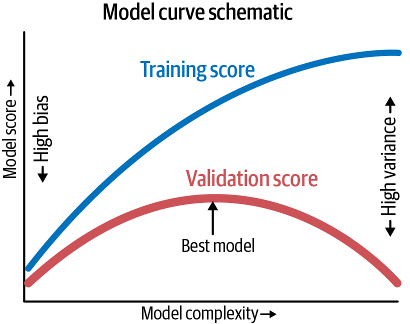
\includegraphics{../img/fig39-5.png}
      \caption{A schematic of the relationship between model complexity, training score, and validation score}
      \label{fig39-5}
\end{figure}

A useful question to answer is this: which model provides a suitable trade-off between bias (underfitting) and
variance (overfitting)?

We can make progress in this by visualizing the validation curve for this particular
data and model; this can be done straightforwardly using the \verb|validation_curve| convenience routine provided by Scikit-Learn. Given a model, data, parameter name,
and a range to explore, this function will automatically compute both the training
score and the validation score across the range.

\section{Learning Curves}
One important aspect of model complexity is that the optimal model will generally
depend on the size of your training data.

The behavior of the validation curve has not one but two important inputs: the
model complexity and the number of training points.

We can gain further insight by
exploring the behavior of the model as a function of the number of training points,
which we can do by using increasingly larger subsets of the data to fit our model. \important{A
      plot of the training/validation score with respect to the size of the training set is
      sometimes known as a \textit{learning curve}.}

The general behavior we would expect from a learning curve is this:
\begin{itemize}
      \item A model of a given complexity will overfit a small dataset: this means the training
            score will be relatively high, while the validation score will be relatively low.
      \item A model of a given complexity will underfit a large dataset: this means that the
            training score will decrease, but the validation score will increase.
      \item A model will never, except by chance, give a better score to the validation set than
            the training set: this means the curves should keep getting closer together but
            never cross.
\end{itemize}

With these features in mind, we would expect a learning curve to look qualitatively
like that shown in \autoref{fig39-11}.

\begin{figure}
      \centering
      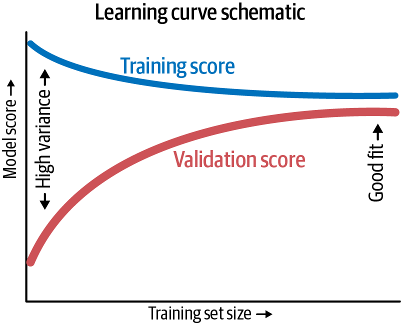
\includegraphics{../img/fig39-11.png}
      \caption{Schematic showing the typical interpretation of learning curves}
      \label{fig39-11}
\end{figure}

The notable feature of the learning curve is the convergence to a particular score as
the number of training samples grows. In particular, once you have enough points
that a particular model has converged, adding more training data will not help you!
The only way to increase model performance in this case is to use another (often
more complex) model.

\figures{Learning curves for a low-complexity model and a high-complexity model}

\autoref{Learning curves for a low-complexity model and a high-complexity model} is a valuable diagnostic, because it gives us a visual depiction of how our model
responds to increasing amounts of training data. In particular, when the learning
curve has already converged (i.e., when the training and validation curves are already
close to each other) adding more training data will not significantly improve the fit!
This situation is seen in the left panel, with the learning curve for the degree-2 model.

The only way to increase the converged score is to use a different (usually more complicated) model. We see this in the right panel: by moving to a much more complicated model, we increase the score of convergence (indicated by the dashed line), but
at the expense of higher model variance (indicated by the difference between the
training and validation scores). If we were to add even more data points, the learning
curve for the more complicated model would eventually converge.

Plotting a learning curve for your particular choice of model and dataset can help you
to make this type of decision about how to move forward in improving your analysis.

\section{Validation in Practice: Grid Search}
GridSearchCV include the ability to specify a custom scoring function, to parallelize the computations, to do randomized searches, and more.
% \chapter{Feature Engineering\label{Ch40}}
In the real world, data rarely comes in such a form. With
this in mind, one of the more important steps in using machine learning in practice is
feature engineering: that is, taking whatever information you have about your problem
and turning it into numbers that you can use to build your feature matrix.
\section{Categorical Features}
One common type of nonnumerical data is categorical data.

The Scikit-Learn's models make the fundamental assumption that numerical features reflect algebraic quantities.

one proven technique is to use one-hot encoding, which effectively creates
extra columns indicating the presence or absence of a category with a value of 1 or 0,
respectively. When your data takes the form of a list of dictionaries, Scikit-Learn's
\verb|DictVectorizer| will do this for you.

To see the meaning of each column, you can inspect the feature names, \verb|get_feature_names_out()|.

There is one clear disadvantage of this approach: if your category has many possible
values, this can greatly increase the size of your dataset. However, because the encoded data contains mostly zeros, a sparse output can be a very efficient solution. Nearly all of the Scikit-Learn estimators accept such sparse inputs when fitting and
evaluating models. Two additional tools that Scikit-Learn includes to support this
type of encoding are \verb|sklearn.preprocessing.OneHotEncoder| and \verb|sklearn.feature_extraction.FeatureHasher|.

\section{Text Features}
Another common need in feature engineering is to convert text to a set of representative numerical values.

\notes{One of the simplest methods of
    encoding this type of data is by \textit{word counts}: you take each snippet of text, count the
    occurrences of each word within it, and put the results in a table.}

There are some issues with using a simple raw word count, however: it can lead to
features that put too much weight on words that appear very frequently, and this can
be suboptimal in some classification algorithms. One approach to fix this is known as
\textit{term frequency–inverse document frequency} (TF–IDF), which weights the word counts
by a measure of how often they appear in the documents.

在一份给定的文件里,词频(term frequency, tf)指的是某一个给定的词语在该文件中出现的频率。这个数字是对词数(term count)的标准化,以防止它偏向长的文件。(同一个词语在长文件里可能会比段文件有更高的次数,而不管该词语重要与否)对于在某一个特定文件里的词语 $t_i$ 来说,它的重要性可表示:
\begin{equation}
    tf_{i,j}=\frac{n_{i,j}}{\sum_k n_{k,j}}
\end{equation}

式中假设文件 $d_j$ 中共有 $k$ 个词语, $n_{k, j}$ 是 $t_k$ 在文件 $d_j$ 中出现的次数。分子 $n_{i,j}$ 是该词在文件 $d_j$ 中出现次数,而分母则是在文件 $d_j$ 中所有字词出现的次数之和。

逆向文件频率(inverse document frequency, idf)是一个词语普遍重要性的度量。某一特定词语的 idf,可以有总文件数目除以包含该词语之文件的数目,再将得到的上取以10为底的对数得到:
\begin{equation}
    idf_i=\log_{10}\frac{|D|}{|\{j:t_i\in d_j\}|}
\end{equation}
式中,$|D|$表示语料库中的文件总数,$|\{j:t_i\in d_j\}|$ 表示包含词语 $t_i$ 的文件数目,如果词语不再资料中,就导致分母为零,因此一般情况下使用$1+ |\{j:t_i\in d_j\}|$,然后
\begin{equation}
    tfidf_{i,j}=tf_{i,j}\times idf_i
\end{equation}
某一特定文件内的高词语频率,以及该词语在整个文件集合中的低文件频率,可以产生出高权重的 $tf-idf$,因此,$tf-idf$ 倾向于过滤掉常见的词语,保留重要的词语。

例子:假如一篇文件的总词数是100个,而词语母牛出现了3次,那么母牛一次在该文件中的词频就 $3/100=0.03$,而计算文件频率的方法就是以文件集的文件总数除以出现母牛一词的文件数,所以,如果母牛一次在1000份文件出现过,而文件总数是10000000份的话,其你想文件频率就是$\log_{10}(10000000/1000)=4$,最后的 $tf-idf$的分数为 $0.03 * 4=.012$,更多访问 \href{https://zh.wikipedia.org/wiki/Tf-idf}{tf-idf}。

\section{Image Features}
Another common need is to suitably encode images for machine learning analysis. A comprehensive summary of feature extraction techniques for images is well beyond
the scope of this chapter, but you can find excellent implementations of many of the
standard approaches in the \href{https://scikit-image.org/}{Scikit-Image project}.

\section{Derived Features}
Another useful type of feature is one that is mathematically derived from some input features. We saw an example of this in \autoref{Ch39} when we constructed \textit{polynomial features} from our input data. We saw that we could convert a linear regression into a polynomial regression not by changing the model, but by transforming the input!

\begin{tcolorbox}
    This idea of improving a model not by changing the model, but by transforming the inputs, is fundamental to many of the more powerful machine learning methods.

    More generally, this is one motivational path to the powerful set of techniques known
    as \textit{kernel methods}.
\end{tcolorbox}

\section{Imputation of Missing Data}
Another common need in feature engineering is handling of missing data. When applying a typical machine learning model to such data, we will need to first
replace the missing values with some appropriate fill value. This is known as \textit{imputation}\marginpar[imputation]{imputation} of missing values, and strategies range from simple (e.g., replacing missing values
with the mean of the column) to sophisticated (e.g., using matrix completion or a robust model to handle such data).

\section{Feature Pipelines}
It can quickly become tedious to do the transformations by hand, especially if you wish to string together multiple steps. Scikit-Learn provides a Pipeline object to streamline type of processing pipeline,
% \chapter{In Depth: Naive Bayes Classification\label{Ch41}}

Naive Bayes models are a group of extremely fast and simple classification algorithms that are often suitable for very high-dimensional datasets. Because they are so fast and have so few tunable parameters, they end up being useful as a quick-and-dirty baseline for a classification problem.

\section{Bayesian Classification}
In Bayesian classification, we’re interested in
finding the probability of a label L given some observed features, which we can write
as $P(L|features)$.

\begin{equation*}
    P(L|features)=\frac{P(features|L)P(L)}{P(features)}
\end{equation*}

If we are trying to decide between two labels—let’s call them $L_1$ and $L_2$—then one way
to make this decision is to compute the ratio of the posterior probabilities for each
label:
\begin{equation*}
    \frac{P(L_1|features)}{P(L_2|features)}=\frac{P(features|L_1)P(L_1)}{P(features|L_2)P(L_2)}
\end{equation*}

All we need now is some model by which we can compute $P(features|L_i)$ for each
label. Such a model is called a \textit{generative model} because it specifies the hypothetical
random process that generates the data. Specifying this generative model for each
label is the main piece of the training of such a Bayesian classifier.

This is where the “naive” in “naive Bayes” comes in: if we make very naive assumptions about the generative model for each label, we can find a rough approximation of
the generative model for each class, and then proceed with the Bayesian classification.
Different types of naive Bayes classifiers rest on different naive assumptions about the
data.

\section{Gaussian Naive Bayes}
Perhaps the easiest naive Bayes classifier to understand is Gaussian naive Bayes. With
this classifier, the assumption is that \textit{data from each label is drawn from a simple Gaussian distribution.}

The simplest Gaussian model is to assume that the data is described by a Gaussian
distribution with no covariance between dimensions. This model can be fit by computing the mean and standard deviation of the points within each label, which is all
we need to define such a distribution.

\figures{Visualization of the Gaussian naive Bayes classification}

\autoref{Visualization of the Gaussian naive Bayes classification}, We see a slightly curved boundary in the classifications—in general, the boundary
produced by a Gaussian naive Bayes model will be quadratic.

A nice aspect of this Bayesian formalism is that it naturally allows for probabilistic classification, which we can compute using the \verb|predict_proba| method. If you are looking for estimates of uncertainty in your classification, Bayesian
approaches like this can be a good place to start.

Of course, the final classification will only be as good as the model assumptions that
lead to it, which is why Gaussian naive Bayes often does not produce very good
results. Still, in many cases—especially as the number of features becomes large—this
assumption is not detrimental enough to prevent Gaussian naive Bayes from being a
reliable method.

\section{Multinomial Naive Bayes}
Another useful example is multinomial naive Bayes, \important{where the features are assumed to be generated from a simple multinomial distribution.} The multinomial distribution describes the probability of observing counts among a number of categories, and thus \notes{multinomial naive Bayes is most appropriate for features that represent counts or count rates.}
\subsection*{Example: Classifying Text}
One place where multinomial naive Bayes is often used is in text classification, where
the features are related to word counts or frequencies within the documents to be
classified.

\section{When to Use Naive Bayes}
Because naive Bayes classifiers make such stringent assumptions about data, they will
generally not perform as well as more complicated models. That said, they have several advantages:
\begin{itemize}
    \item They are fast for both training and prediction.
    \item They provide straightforward probabilistic prediction.
    \item They are often easily interpretable.
    \item They have few (if any) tunable parameters.
\end{itemize}

Naive Bayes classifiers tend to perform especially well in the following situations:
\begin{itemize}
    \item When the naive assumptions actually match the data (very rare in practice)
    \item For very well-separated categories, when model complexity is less important
    \item For very high-dimensional data, when model complexity is less important
\end{itemize}
The last two points seem distinct, but they actually are related: as the dimensionality of a dataset grows, it is much less likely for any two points to be found close together (\tips{after all, they must be close in every single dimension to be close overall}). This means that clusters in high dimensions tend to be more separated, on average, than clusters in low dimensions, assuming the new dimensions actually add information.
% \chapter{In Depth: Linear Regression\label{Ch42}}
Just as naive Bayes (discussed in \autoref{Ch41}) is a good starting point for classification
tasks, linear regression models are a good starting point for regression tasks. Such
models are popular because they can be fit quickly and are straightforward to interpret.
\section{Simple Linear Regression}
We can use the single LinearRegression estimator to fit lines, planes, or
hyperplanes to our data. It still appears that this approach would be limited to strictly
linear relationships between variables.

\section{Basis Function Regression}
One trick you can use to adapt linear regression to nonlinear relationships between variables is to transform the data according to basis functions. We have seen one version of this before, in the PolynomialRegression pipeline used in \autoref{Ch39} and \autoref{Ch40}. The idea is to take our multidimensional linear model:
\begin{equation*}
    y = a_0 + a_1x_1 + a_2x_2 + a_3x_3 +\cdots
\end{equation*}
and build the $x_1, x_2, x_3$, and so on from our single-dimensional input $x$. That is, we let
$x_n = f_n(x)$ , where $f_n$ is some function that transforms our data.(这个多元回归模型中,特征都是一维输入的函数) For example, if $f_n(x) = x^n$, our model becomes a polynomial regression:
\begin{equation*}
    y = a_0 + a_1x + a_2x^2 + a_3x^3 +\cdots
\end{equation*}
Notice that this is still a linear model—\important{the linearity refers to the fact that the coefficients an never multiply or divide each other.} What we have effectively done is taken
our one-dimensional x values and projected them into a higher dimension, so that a linear fit can fit more complicated relationships between $x$ and $y$.

\subsection*{Polynomial Basis Functions}
This polynomial projection is useful enough that it is built into Scikit-Learn, using the PolynomialFeatures transformer.

\subsection*{Gaussian Basis Functions}
Of course, other basis functions are possible. For example, one useful pattern is to fit a model that is not a sum of polynomial bases, but a sum of Gaussian bases. The result might look something like \autoref{A Gaussian basis function fit to nonlinear data}.

Algebraically, Gaussian basis functions are defined as follows:
\begin{equation}
    \phi_k(t;\mu_k ,\sigma^2_k) = \exp \left(-\dfrac{||t-\mu_k||^2}{2\sigma^2_k}\right), k=1,\dots,K
\end{equation}
where$\mu_k$is a parameter determining the center of the basis function,$\sigma_k^2$
is a parameter that determines the width and $||.||$ is the Euclidian norm. The basis functions overlap with each other to capture the information about $t$, and the width parameter play an essential role to capture the structure in the data over the region of input data. The parameters featuring in each basis function are often determined heuristically based on the structure of the observed data.

\figures{A Gaussian basis function fit to nonlinear data}

The shaded regions in the \autoref{A Gaussian basis function fit to nonlinear data} are the scaled basis functions, and when added together they reproduce the smooth curve through the data. These Gaussian basis functions are not built into Scikit-Learn, but we can write a custom transformer that
will create them.

\section{Regularization}
The introduction of basis functions into our linear regression makes the model much more flexible, but it also can very quickly lead to overfitting.

We know that such
behavior is problematic, and it would be nice if we could limit such spikes explicitly
in the model by penalizing large values of the model parameters. Such a penalty is
known as regularization, and comes in several forms.

\subsection*{Ridge Regression ($L_2$ Regularization)}
Perhaps the most common form of regularization is known as ridge regression or $L_2$ regularization (sometimes also called Tikhonov regularization). This proceeds by penalizing the sum of squares (2-norms) of the model coefficients θn. In this case, the
penalty on the model fit would be:
\begin{equation}
    P=\alpha\sum_{i=1}^{n}\theta_n^2
\end{equation}
where $\alpha$ is a free parameter that controls the strength of the penalty. This type of penalized model is built into Scikit-Learn with the \verb|Ridge|\marginpar[Ridge]{Ridge} estimator.

\subsection*{Lasso Regression ($L_1$ Regularization)}
Another common type of regularization is known as lasso regression or $L_1$ regularization and involves penalizing the sum of absolute values (1-norms) of regression
coefficients:
\begin{equation}
    P=\alpha\sum_{i=1}^{n}|\theta_n|
\end{equation}
Though this is conceptually very similar to ridge regression, the results can differ surprisingly. For example, \tips{due to its construction, lasso regression tends to favor sparse models where possible: that is, it preferentially sets many model coefficients to exactly zero.}
% \chapter{In Depth: Support Vector Machines\label{Ch43}}
Support vector machines (SVMs) are a particularly powerful and flexible class of
supervised algorithms for both classification and regression.
\section{Motivating Support Vector Machines}
As part of our discussion of Bayesian classification (see \autoref{Ch41}), we learned about a simple kind of model that describes the distribution of each underlying class, and experimented with using it to probabilistically determine labels for new points. That was an example of generative classification; here we will consider instead discriminative classification. That is, rather than modeling each class, we will simply find a line or curve (in two dimensions) or manifold (in multiple dimensions) that divides the classes from each other.

\figures{Three perfect linear discriminative classifiers for our data}

These are three very different separators which, nevertheless, perfectly discriminate between these samples. Depending on which you choose, a new data point (e.g., the one marked by the “X” in \autoref{Three perfect linear discriminative classifiers for our data}) will be assigned a different label! Evidently our simple intuition of “drawing a line between classes” is not good enough, and we need to think a bit more deeply.
\section{Support Vector Machines: Maximizing the Margin}
Support vector machines offer one way to improve on this. The intuition is this: rather than simply drawing a zero-width line between the classes, we can draw around each line a \textit{margin}\marginpar[margin]{margin} of some width, up to the nearest point. \important{The line that maximizes this margin is the one we will choose as the optimal model.}

\subsection*{Fitting a Support Vector Machine}
Let’s see the result of an actual fit to this data: we will use Scikit-Learn’s support vector classifier (SVC) to train an SVM model on this data.

A key to this classifier’s success is that for the fit, only the positions of the support vectors matter; any points further from the margin that are on the correct side do not modify the fit. Technically, this is because these points do not contribute to the loss function used to fit the model, so their position and number do not matter so long as they do not cross the margin.

\figures{The influence of new training points on the SVM model}

\autoref{The influence of new training points on the SVM model}, in the left panel, we see the model and the support vectors for 60 training points. In
the right panel, we have doubled the number of training points, but the model has
not changed: the three support vectors in the left panel are the same as the support
vectors in the right panel. \important{This insensitivity to the exact behavior of distant points is one of the strengths of the SVM model.}
\subsection*{Beyond Linear Boundaries: Kernel SVM}
Where SVM can become quite powerful is when it is combined with \textit{kernels}. There we projected our data into a higher-dimensional space defined by polynomials
and Gaussian basis functions, and thereby were able to fit for nonlinear relationships
with a linear classifier.
\subsection*{Tuning the SVM: Softening Margins}



% \chapter{In Depth: Decision Trees and Random Forests\label{Ch44}}
Here we'll take a look at another powerful algorithm: a nonparametric
algorithm called random forests. Random forests are an example of an ensemble
method, meaning one that relies on aggregating the results of a set of simpler estimators.

\section{Summary}
A primary disadvantage of random forests is that the results are not easily interpretable: that is, if you would like to draw conclusions about the meaning of the classification model, random forests may not be the best choice.


% \chapter{In Depth: Principal Component Analysis\label{Ch45}}

\section{Introducing Principal Component Analysis}
These vectors represent the principal axes of the data, and the length of each vector is
an indication of how “important” that axis is in describing the distribution of the data
—more precisely, it is a measure of the variance of the data when projected onto that
axis. The projection of each data point onto the principal axes are the principal components of the data.

This transformation from data axes to principal axes is an \textbf{affine transformation},
which means it is composed of a translation, rotation, and uniform scaling.

\subsection{PCA as Dimensionality Reduction}
Using PCA for dimensionality reduction involves zeroing out one or more of the
smallest principal components, resulting in a lower-dimensional projection of the
data that preserves the maximal data variance.

\subsection{What Do the Components Mean?}
We can go a bit further here, and begin to ask what the reduced dimensions mean.
This meaning can be understood in terms of combinations of basis vectors.
\subsection{Choosing the Number of Components}
A vital part of using PCA in practice is the ability to estimate how many components are needed to describe the data. This can be determined by looking at the cumulative \textbf{explained variance ratio} as a function of the number of components.

\begin{figure}
    \centering
    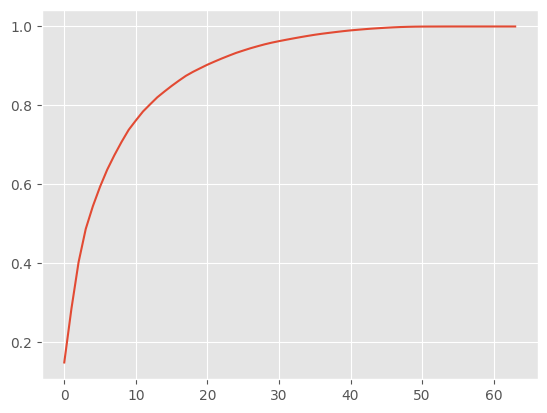
\includegraphics{../img/fig45-8.png}
    \caption{The cumulative explained variance, which measures how well PCA preserves the content of the data}
\end{figure}

This tells us that our two-dimensional projection loses a lot of information (as measured by the explained variance) and that we'd need about 20 components to retain
90\% of the variance. Looking at this plot for a high-dimensional dataset can help you
understand the level of redundancy present in its features.

\section{PCA as Noise Filtering}
PCA can also be used as a filtering approach for noisy data. The idea is this: any components with variance much larger than the effect of the noise should be relatively unaffected by the noise. So, if you reconstruct the data using just the largest subset of principal components, you should be preferentially keeping the signal and throwing out the noise.

\section{Example: Eigenfaces}
In this case, it can be interesting to visualize the images associated with the first several principal components (these components are technically known as \textbf{eigenvectors}, so these types of images are often called \textbf{eigenfaces}; as you can see in \autoref{A visualization of eigenfaces learned from the LFW dataset}, they are as creepy as they sound)
\figures{A visualization of eigenfaces learned from the LFW dataset}

The results are very interesting, and give us insight into how the images vary: for example, the first few eigenfaces (from the top left) seem to be associated with the angle of lighting on the face, and later principal vectors seem to be picking out certain features, such as eyes, noses, and lips.

\section{Summary}

Given any high-dimensional dataset, I tend to start with PCA in order to visualize the relationships between points (as we did with the digits data), to understand the main variance in the data (as we did with the eigenfaces), and to understand the intrinsic dimensionality (by plotting the explained variance ratio). Certainly PCA is not useful for every high-dimensional dataset, but it offers a straightforward and efficient path to gaining insight into high-dimensional data.

\important{PCA's main weakness is that it tends to be highly affected by outliers in the data.} For this reason, several robust variants of PCA have been developed, many of which act to iteratively discard data points that are poorly described by the initial components.
% \chapter{In Depth: Manifold Learning\label{Ch46}}
While PCA is flexible, fast, and easily interpretable, it does
not perform so well when there are nonlinear relationships within the data.

\section{Multidimensional Scaling}
Given a distance matrix between points, it recovers a D-dimensional coordinate representation
of the data, this is exactly what the multidimensional scaling algorithm aims to do.

\subsection{MDS as Manifold Learning}

This is essentially the goal of a manifold learning estimator: given high-dimensional
embedded data, it seeks a low-dimensional representation of the data that preserves
certain relationships within the data. In the case of MDS, the quantity preserved is the
distance between every pair of points.

\begin{figure}
    \centering
    \begin{subfigure}[b]{.45\textwidth}
        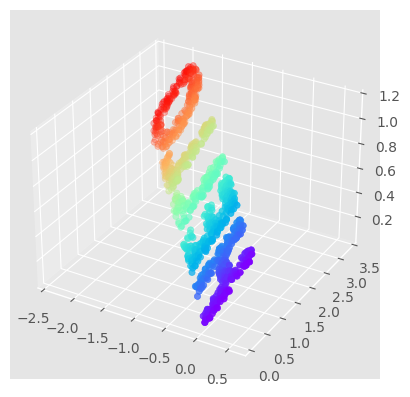
\includegraphics[width=\textwidth]{../img/fig46-5.png}
        \caption{Data embedded linearly into three dimensions}
    \end{subfigure}
    \hfill
    \begin{subfigure}[b]{.45\textwidth}
        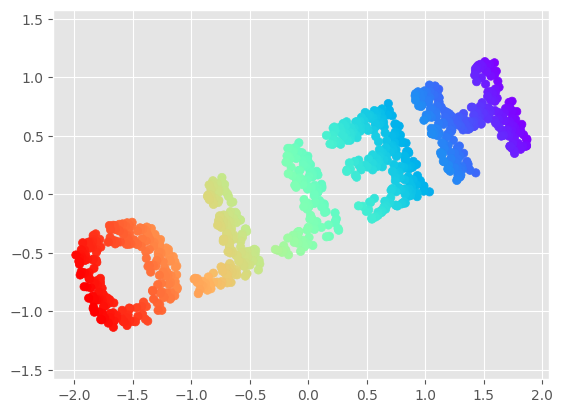
\includegraphics[width=\textwidth]{../img/fig46-6.png}
        \caption{The MDS embedding of the three-dimensional data recovers the input up to a rotation and reflection}
    \end{subfigure}
    \caption{MDS as Manifold Learning}
\end{figure}

\subsection{Nonlinear Embeddings: Where MDS Fails}
Where MDS breaks down is when the embedding is nonlinear—that is, when it goes beyond this simple set of operations.

\section{Nonlinear Manifolds: Locally Linear Embedding}
MDS tries to preserve distances between faraway points when constructing the embedding. But what if we instead modified the algorithm such that it
only preserves distances between nearby points? The resulting embedding would be
closer to what we want.

\begin{figure}
    \centering
    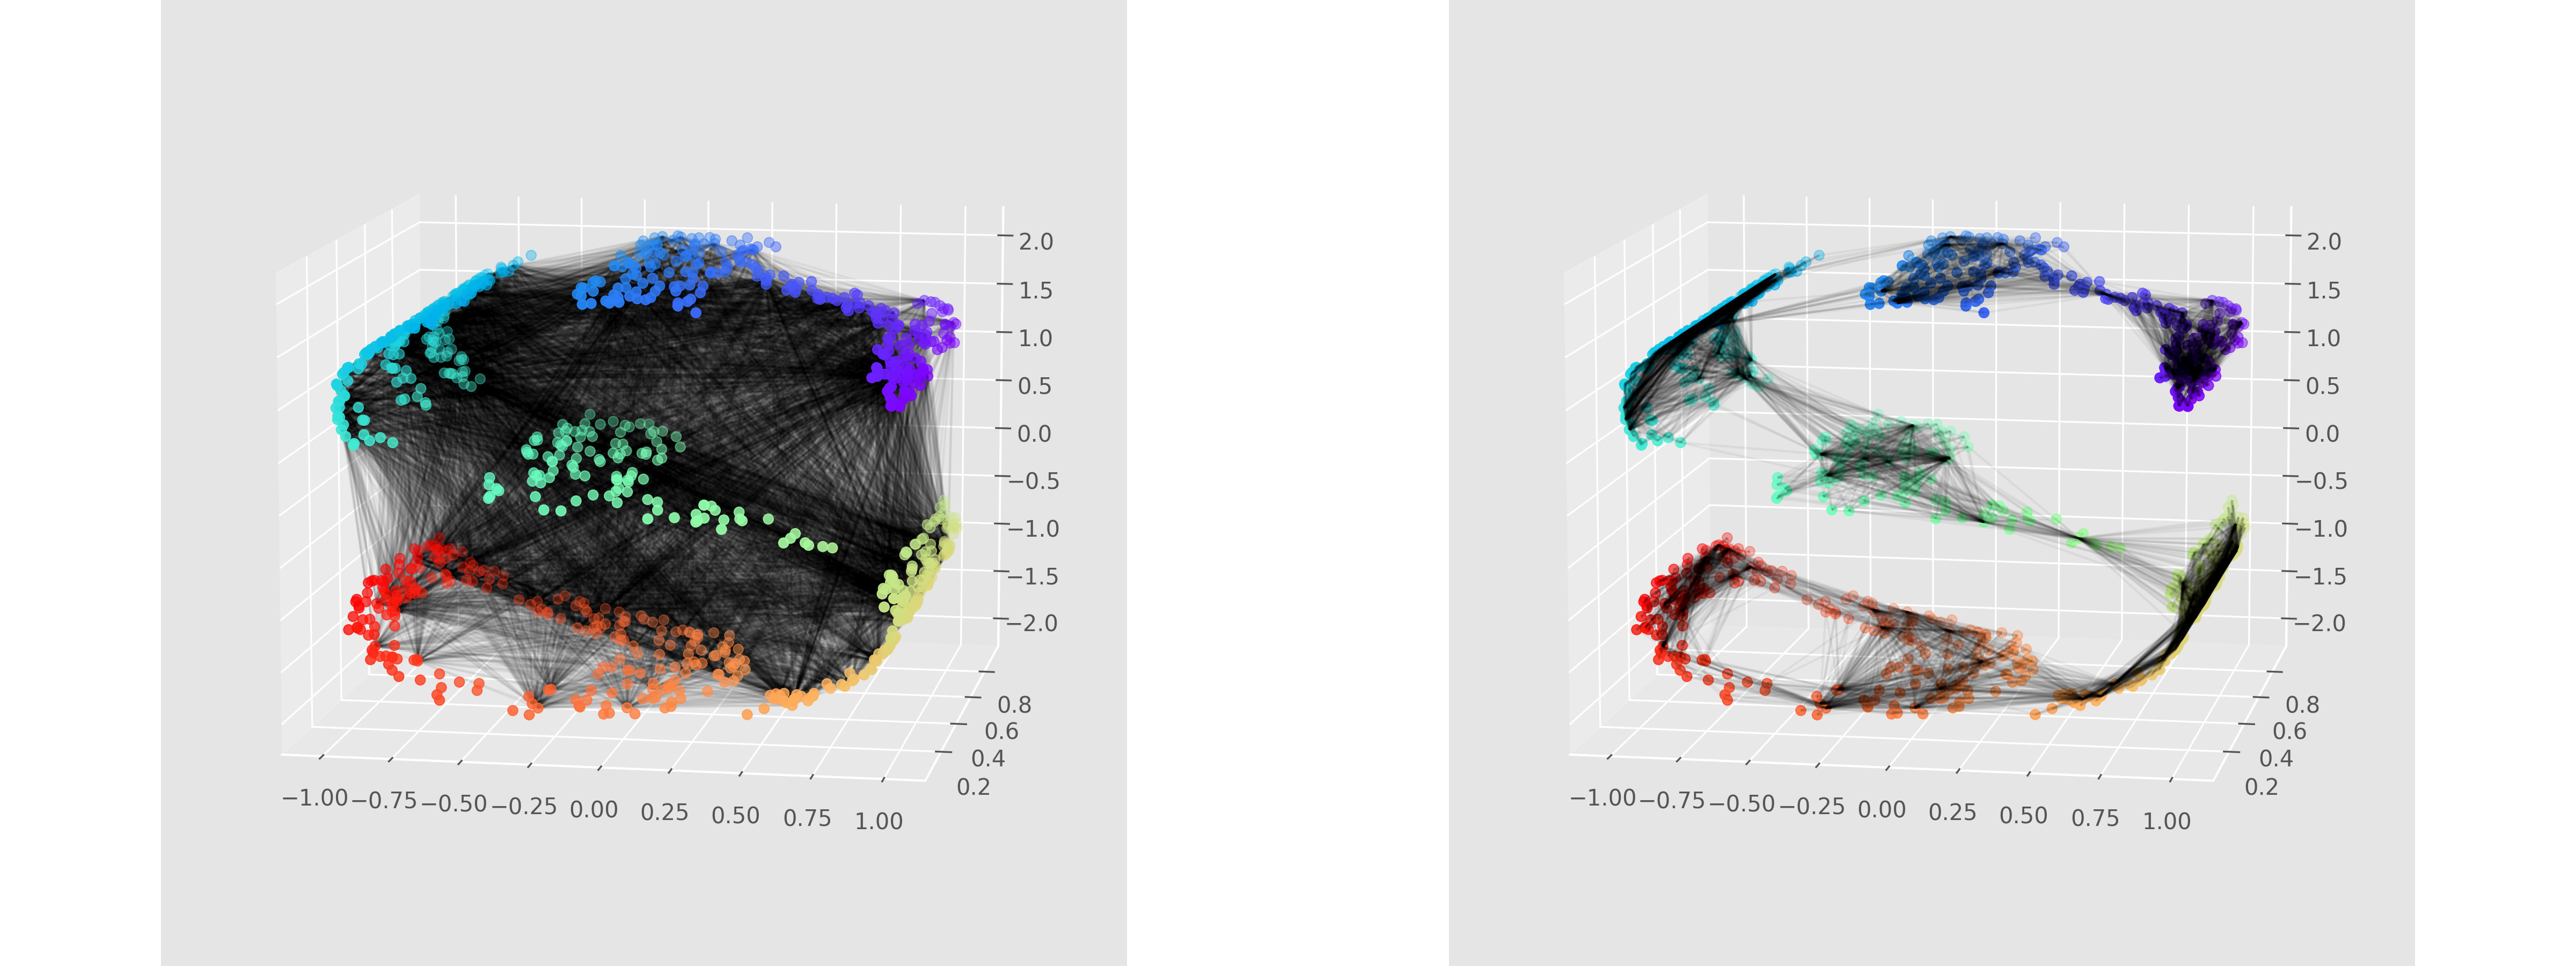
\includegraphics[width=\textwidth]{../img/fig46-7.png}
    \caption{Representation of linkages between points within MDS and LLE}
\end{figure}

\section{Some Thoughts on Manifold Methods}
In practice manifold learning techniques tend
to be finicky enough that they are rarely used for anything more than simple qualitative visualization of high-dimensional data.

The following are some of the particular challenges of manifold learning, which all
contrast poorly with PCA:
\begin{itemize}
    \item In manifold learning, there is no good framework for handling missing data. In contrast, there are straightforward iterative approaches for dealing with missing data in PCA.
    \item In manifold learning, the presence of noise in the data can “short-circuit” the manifold and drastically change the embedding. In contrast, PCA naturally filters noise from the most important components.
    \item The manifold embedding result is generally highly dependent on the number of neighbors chosen, and there is generally no solid quantitative way to choose an optimal number of neighbors. In contrast, PCA does not involve such a choice.
    \item In manifold learning, the globally optimal number of output dimensions is difficult to determine. In contrast, PCA lets you find the number of output dimensions based on the explained variance.
    \item In manifold learning, the meaning of the embedded dimensions is not always clear. In PCA, the principal components have a very clear meaning.
    \item In manifold learning, the computational expense of manifold methods scales as $O[N^2]$ or $O[N^3]$ . For PCA, there exist randomized approaches that are generally much faster (though see the \href{https://github.com/mmp2/megaman}{megaman package} for some more scalable implementations of manifold learning).
\end{itemize}

Based on my own experience, I would give the following recommendations:

\begin{itemize}
    \item For toy problems such as the S-curve we saw before, LLE and its variants (especially modified LLE) perform very well. This is implemented in sklearn.manifold.LocallyLinearEmbedding.
    \item For high-dimensional data from real-world sources, LLE often produces poor results, and Isomap seems to generally lead to more meaningful embeddings. This is implemented in sklearn.manifold.Isomap.
    \item For data that is highly clustered, t-distributed stochastic neighbor embedding (t-SNE) seems to work very well, though it can be very slow compared to other methods. This is implemented in sklearn.manifold.TSNE.
\end{itemize}
% \chapter{In Depth: k-Means Clustering\label{Ch47}}
Now we will move on to another class of unsupervised
machine learning models: clustering algorithms. Clustering algorithms seek to learn,
from the properties of the data, an optimal division or discrete labeling of groups of
points.
\section{Introducing k-Means}
The k-means algorithm searches for a predetermined number of clusters within an
unlabeled multidimensional dataset. It accomplishes this using a simple conception of
what the optimal clustering looks like:
\begin{itemize}
    \item The \textbf{cluster center} is the arithmetic mean of all the points belonging to the cluster.
    \item Each point is closer to its own cluster center than to other cluster centers.
\end{itemize}
Those two assumptions are the basis of the k-means model.

\section{Expectation–Maximization}
In short,
the expectation–maximization approach in k-means consists of the following procedure:
\begin{enumerate}
    \item Guess some cluster centers.
    \item Repeat until converged:
          \begin{enumerate}
              \item E-step: Assign points to the nearest cluster center.
              \item M-step: Set the cluster centers to the mean of their assigned points.
          \end{enumerate}
\end{enumerate}
Here the E-step or expectation step is so named because it involves updating our
expectation of which cluster each point belongs to. The M-step or maximization step
is so named because it involves maximizing some fitness function that defines the
locations of the cluster centers—in this case, that maximization is accomplished by
taking a simple mean of the data in each cluster.

There are a few caveats to be aware of when using the expectation–maximization
algorithm:
\paragraph{\textit{The globally optimal result may not be achieved}} First, although the E–M procedure is guaranteed to improve the result in each
step, there is no assurance that it will lead to the global best solution.

\paragraph{\textit{The number of clusters must be selected beforehand}} Another common challenge with k-means is that you must tell it how many clusters you expect: it cannot learn the number of clusters from the data.

Whether the result is meaningful is a question that is difficult to answer definitively; one approach that is rather intuitive, but that we won’t discuss further
here, is called \href{https://scikit-learn.org/stable/auto_examples/cluster/plot_kmeans_silhouette_analysis.html}{silhouette analysis}.

Alternatively, you might use a more complicated clustering algorithm that has a
better quantitative measure of the fitness per number of clusters (e.g., Gaussian
mixture models;) or which can choose a suitable number of clusters (e.g., DBSCAN, mean-shift, or affinity propagation, all available in the
sklearn.cluster submodule).

\paragraph{\textit{k-means is limited to linear cluster boundaries}} The fundamental model assumptions of k-means (points will be closer to their own cluster center than to others) means that the algorithm will often be ineffective if the clusters have complicated geometries.

\figures{Failure of k-means with nonlinear boundaries}

\paragraph{\textit{k-means can be slow for large numbers of samples}} Because each iteration of k-means must access every point in the dataset, the
algorithm can be relatively slow as the number of samples grows. You might
wonder if this requirement to use all data at each iteration can be relaxed; for
example, you might just use a subset of the data to update the cluster centers at
each step. This is the idea behind batch-based k-means algorithms, one form of
which is implemented in sklearn.cluster.MiniBatchKMeans.
\chapter{In Depth: Gaussian Mixture Models\label{Ch48}}
In particular, the nonprobabilistic nature of k-means and its use of simple
distance from cluster center to assign cluster membership leads to poor performance
for many real-world situations. Gaussian mixture models can be viewed as an extension of the ideas behind k-means, but can
also be a powerful tool for estimation beyond simple clustering.

An important observation for k-means is that these cluster models must be circular: k-means has no built-in way of accounting for oblong or elliptical clusters.

\begin{figure}
    \centering
    \begin{subfigure}[f]{.45\textwidth}
        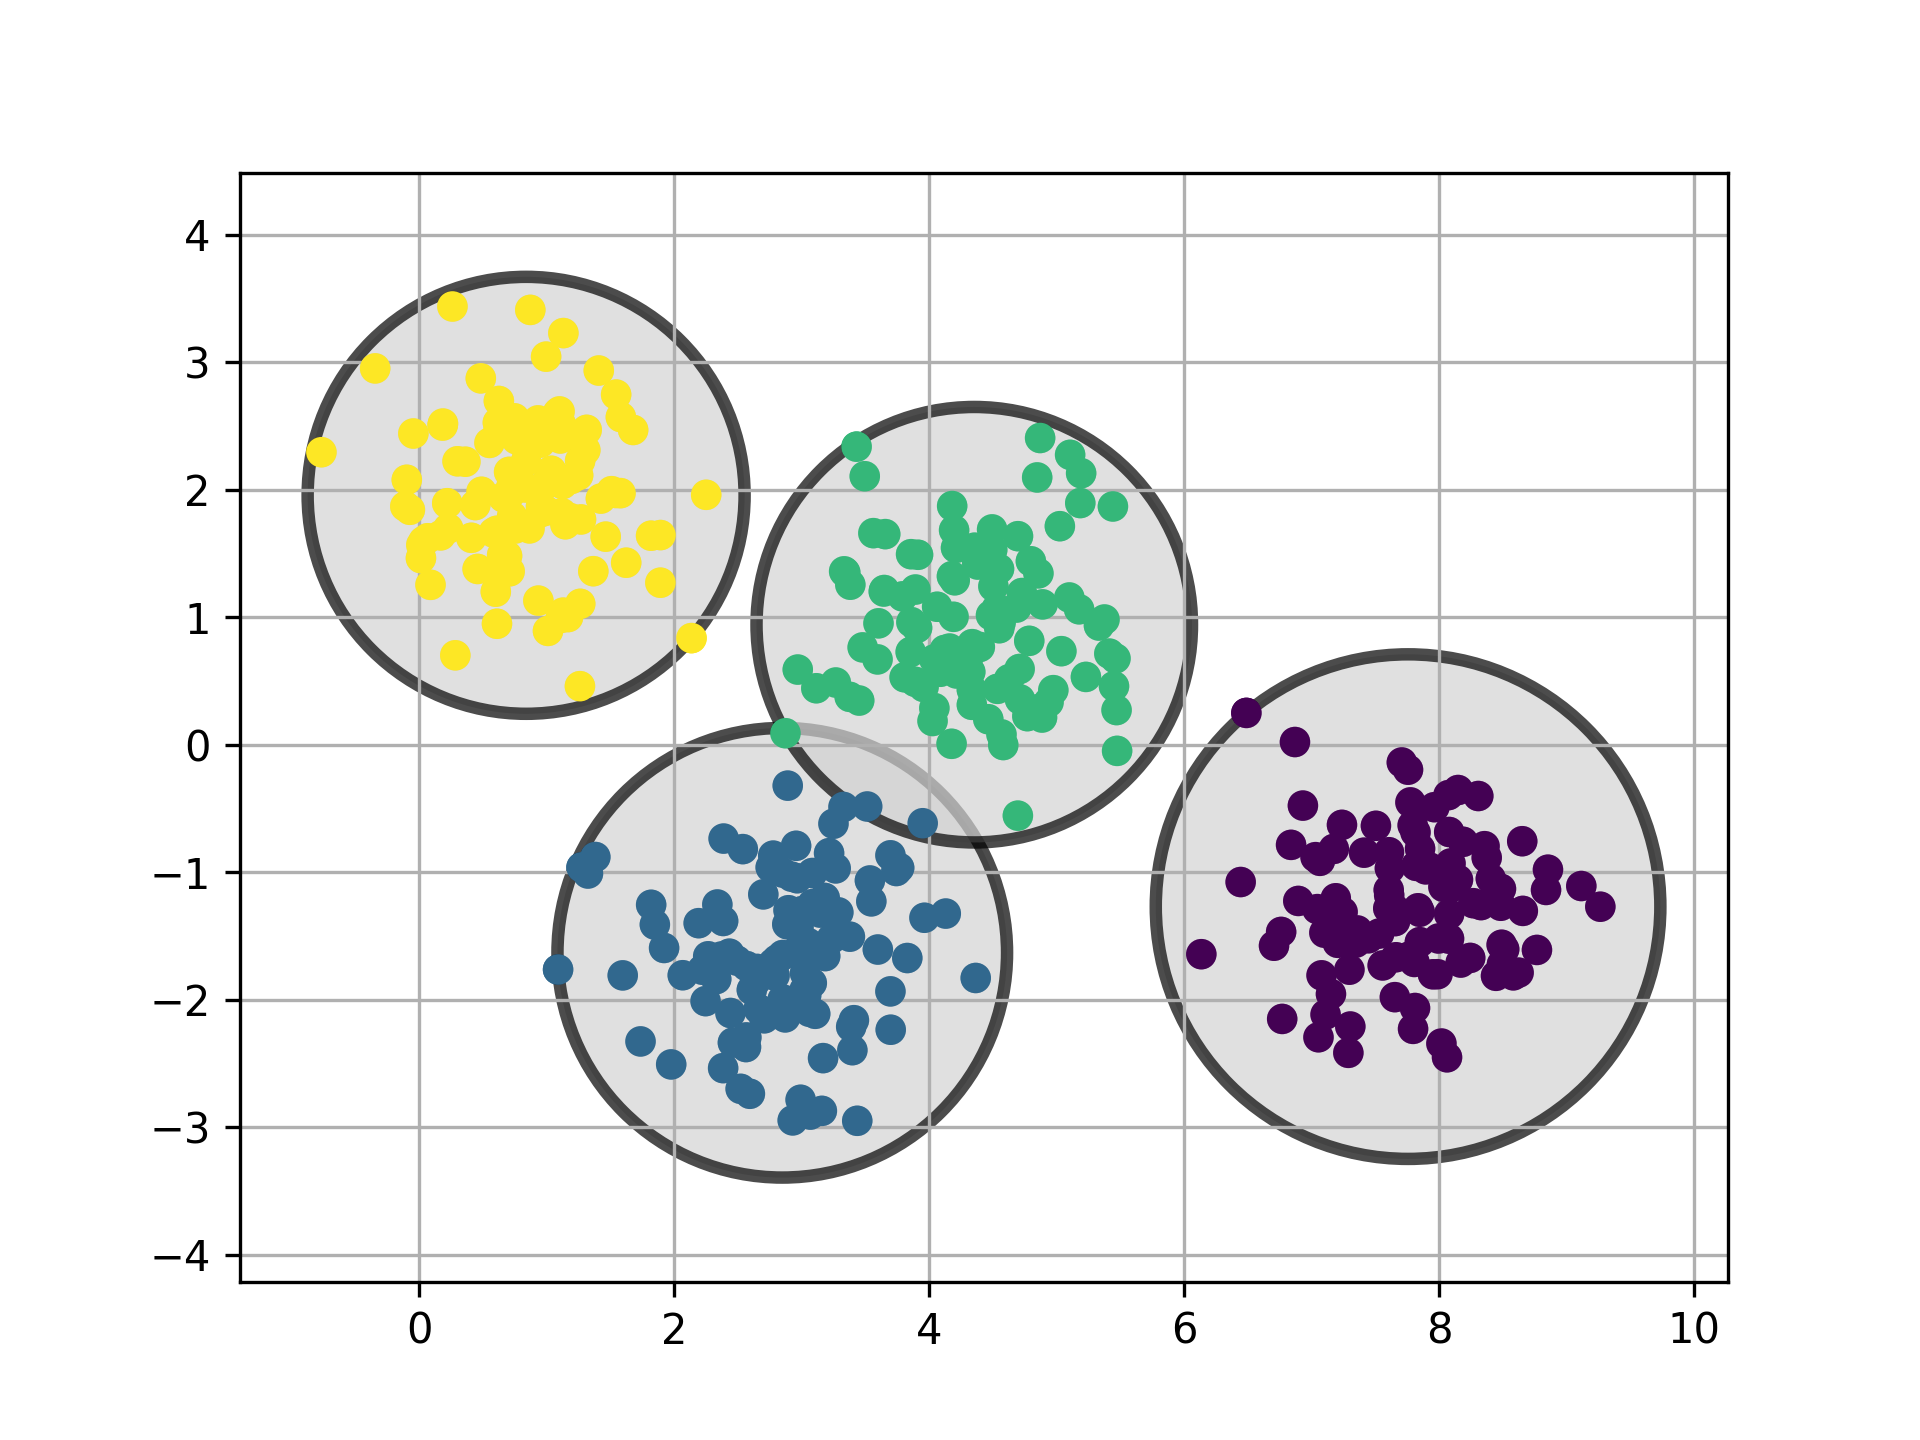
\includegraphics[width=\textwidth]{../Figures/fig48-2.png}
        \caption{The circular clusters implied by the k-means model}
    \end{subfigure}
    \hfill
    \begin{subfigure}[f]{.45\textwidth}
        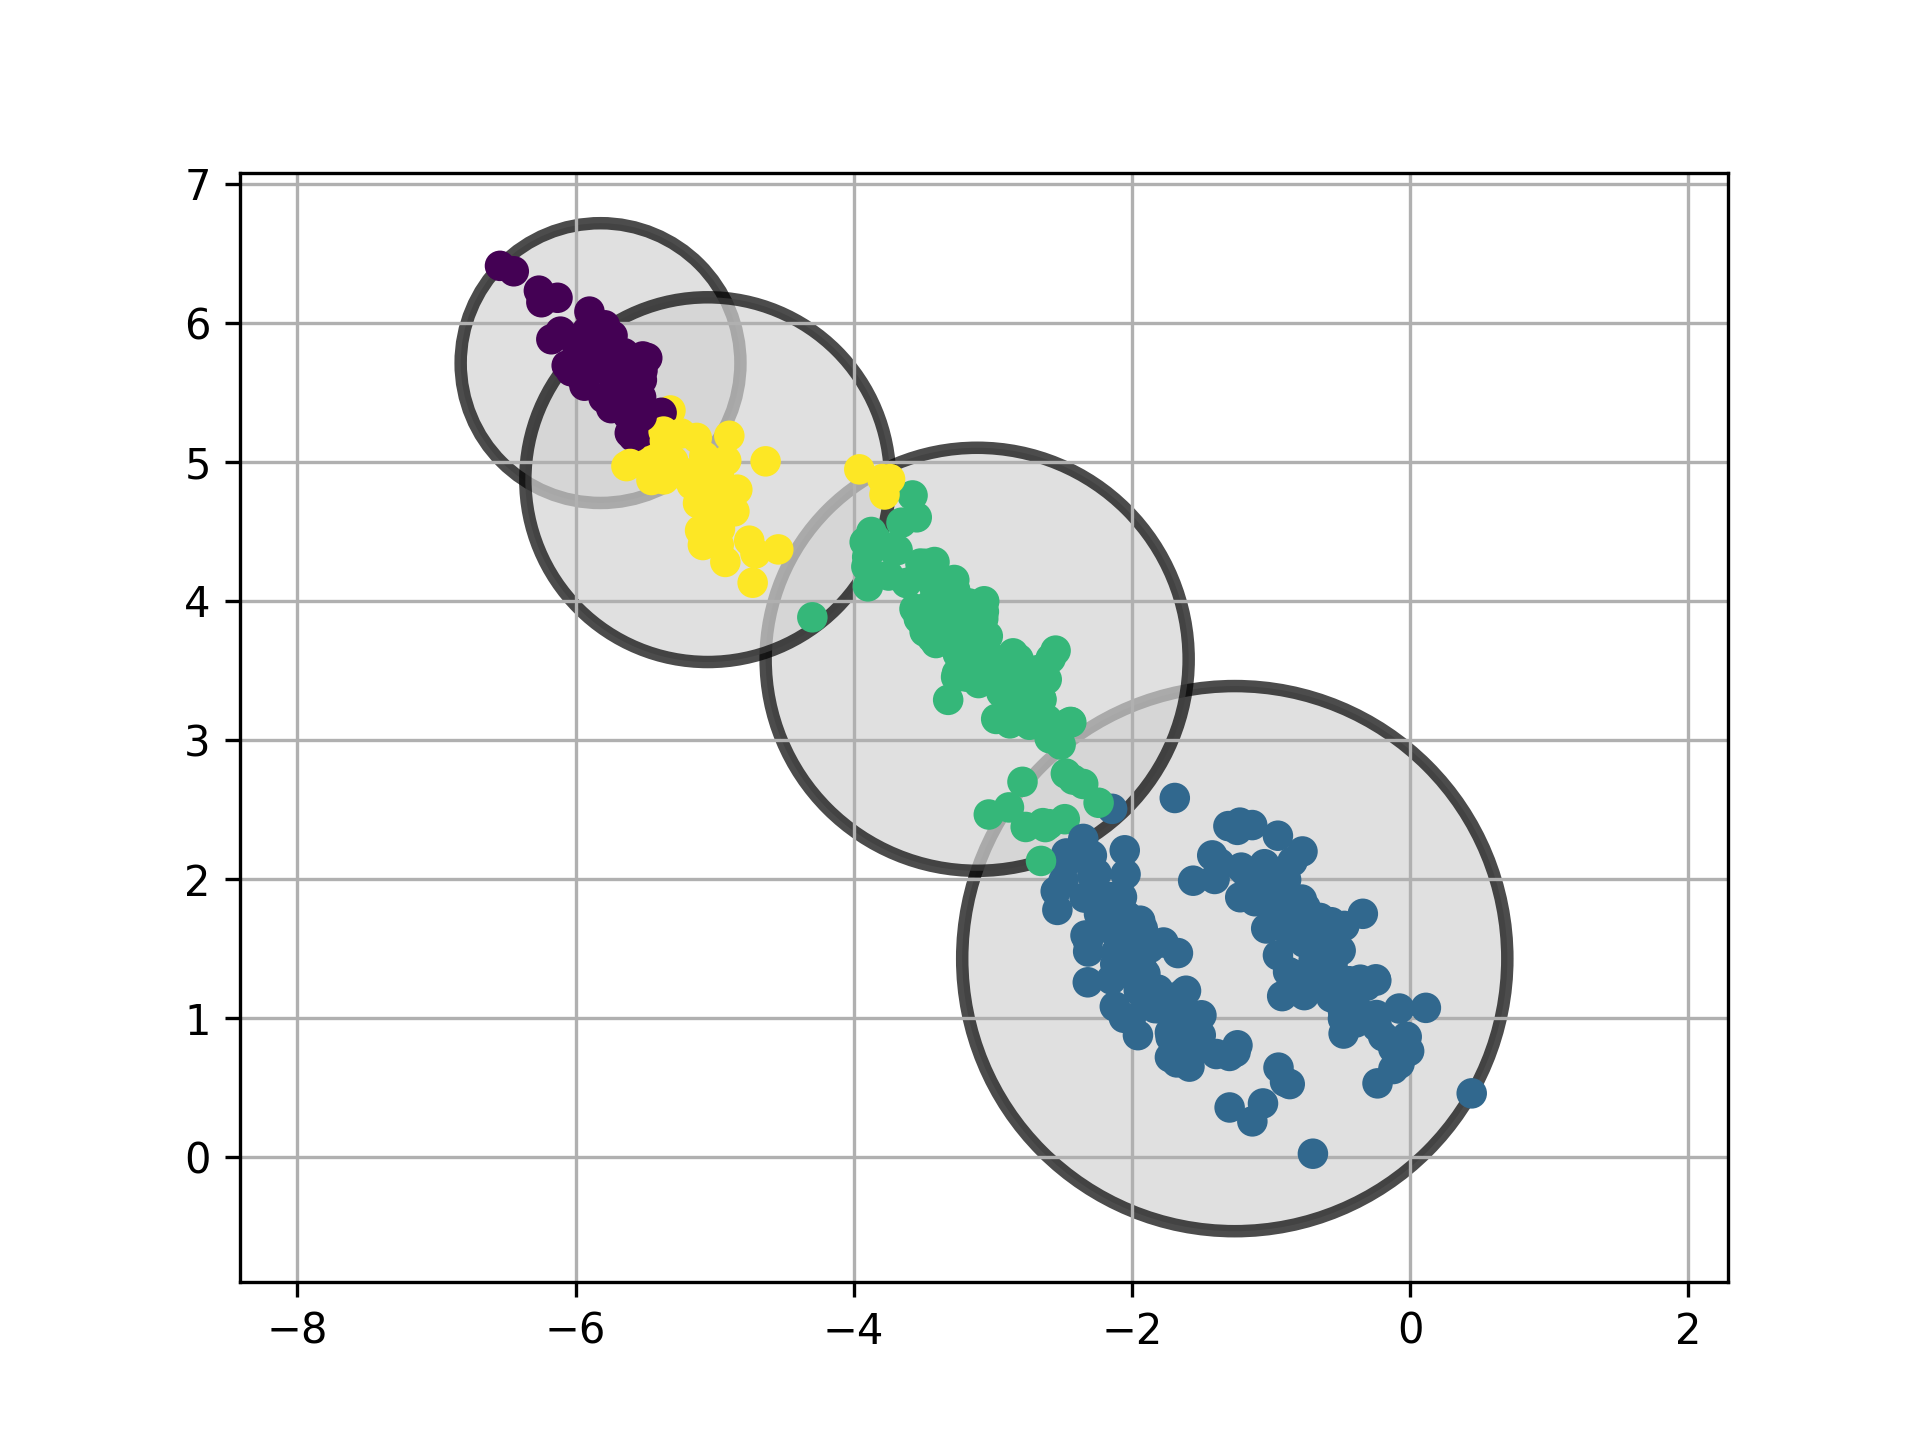
\includegraphics[width=\textwidth]{../Figures/fig48-3.png}
        \caption{Poor performance of k-means for noncircular clusters}
    \end{subfigure}
    \caption{Motivating Gaussian Mixtures: Weaknesses of k-Means}
\end{figure}

These two disadvantages of k-means—its \important{lack of flexibility in cluster shape and lack of probabilistic cluster assignment}—mean that for many datasets (especially low-dimensional datasets) it may not perform as well as you might hope.

\section{Generalizing E–M: Gaussian Mixture Models}
A \textbf{Gaussian mixture model} (GMM) attempts to find a mixture of multidimensional
Gaussian probability distributions that best model any input dataset.

Under the hood, a Gaussian mixture model is very similar to k-means: it uses an
expectation–maximization approach, which qualitatively does the following:
\begin{enumerate}
    \item Choose starting guesses for the location and shape.
    \item Repeat until converged:
          \begin{enumerate}
              \item E-step: For each point, find weights encoding the probability of membership in each cluster.
              \item M-step: For each cluster, update its location, normalization, and shape based on all data points, making use of the weights.
          \end{enumerate}
\end{enumerate}
The result of this is that each cluster is associated not with a hard-edged sphere, but
with a smooth Gaussian model. Just as in the k-means expectation–maximization
approach, this algorithm can sometimes miss the globally optimal solution, and thus
in practice multiple random initializations are used.

\section{Choosing the Covariance Type}
If you look at the details of the preceding fits, you will see that the \verb|covariance_type| option was set differently within each. This hyperparameter controls the degrees of freedom in the shape of each cluster; it's essential to set this carefully for any given problem. The default is \verb|covariance_type="diag"|, which means that the size of the cluster along each dimension can be set independently, with the resulting ellipse constrained to align with the axes. \verb|covariance_type="spherical"| is a slightly simpler and faster model, which constrains the shape of the cluster such that all dimensions
are equal. The resulting clustering will have similar characteristics to that of k-means,
though it's not entirely equivalent. A more complicated and computationally expensive model (especially as the number of dimensions grows) is to use \verb|covariance_type="full"|, which allows each cluster to be modeled as an ellipse with arbitrary orientation.

\section{Gaussian Mixture Models as Density Estimation}
Though the GMM is often categorized as a clustering algorithm, fundamentally it is an algorithm for density estimation. That is to say, the result of a GMM fit to some data is technically not a clustering model, but a generative probabilistic model describing the distribution of the data.

A GMM is convenient as a flexible means of modeling an arbitrary multidimensional
distribution of data.
The fact that a GMM is a generative model gives us a natural means of determining
the optimal number of components for a given dataset. A generative model is inherently a probability distribution for the dataset, and so we can simply evaluate the likelihood of the data under the model, using cross-validation to avoid overfitting.
Another means of correcting for overfitting is to adjust the model likelihoods using
some analytic criterion such as the \href{https://en.wikipedia.org/wiki/Akaike_information_criterion}{Akaike information criterion (AIC)} or \href{https://en.wikipedia.org/wiki/Bayesian_information_criterion}{the Bayesian information criterion (BIC)}.
\end{document}